\documentclass[11pt,a4paper]{report}%especifica o tipo de documento que tenciona escrever: carta, artigo, relatório... neste caso é um relatório
% [11pt,a4paper] Define o tamanho principal das letras do documento. caso não especifique uma delas, é assumido 10pt
% a4paper -- Define o tamanho do papel.
\usepackage{float}
\usepackage[portuges]{babel}%Babel -- irá activar automaticamente as regras apropriadas de hifenização para a língua todo o
                                   %-- o texto gerado é automaticamente traduzido para Português.
                                   %  Por exemplo, “chapter” irá passar a “capítulo”, “table of contents” a “conteúdo”.
                                   % portuges -- específica para o Português.
\usepackage[utf8]{inputenc} % define o encoding usado texto fonte (input)--usual "utf8" ou "latin1

\usepackage{graphicx} %permite incluir graficos, tabelas, figuras
\usepackage{url} % para utilizar o comando \url{}
\usepackage{enumerate} %permite escolher, nas listas enumeradas, se os iems sao marcados com letras ou numeros-romanos em vez de numeracao normal

%\usepackage{apalike} % gerar biliografia no estilo 'named' (apalike)

\usepackage{color} % Para escrever em cores
\usepackage{tabularx}

\usepackage{multirow} %tabelas com multilinhas
\usepackage{array} %formatação especial de tabelas em array

\usepackage[pdftex]{hyperref} % transformar as referências internas do seu documento em hiper-ligações.

%Exemplos de fontes -- nao e vulgar mudar o tipo de fonte
%\usepackage{tgbonum} % Fonte de letra: TEX Gyre Bonum
%\usepackage{lmodern} % Fonte de letra: Latin Modern Sans Serif
%\usepackage{helvet}  % Fonte de letra: Helvetica
%\usepackage{charter} % Fonte de letra:Charter

\definecolor{saddlebrown}{rgb}{0.55, 0.27, 0.07} % para definir uma nova cor, neste caso 'saddlebrown'

\usepackage{listings}  % para utilizar blocos de texto verbatim no estilo 'listings'
%paramerização mais vulgar dos blocos LISTING - GENERAL
\lstset{
	basicstyle=\small, %o tamanho das fontes que são usadas para o código
	numbers=left, % onde colocar a numeração da linha
	numberstyle=\tiny, %o tamanho das fontes que são usadas para a numeração da linha
	numbersep=5pt, %distancia entre a numeração da linha e o codigo
	breaklines=true, %define quebra automática de linha
    frame=tB,  % caixa a volta do codigo
	mathescape=true, %habilita o modo matemático
	escapeinside={(*@}{@*)} % se escrever isto  aceita tudo o que esta dentro das marcas e nao altera
}
%
%\lstset{ %
%	language=Java,							% choose the language of the code
%	basicstyle=\ttfamily\footnotesize,		% the size of the fonts that are used for the code
%	keywordstyle=\bfseries,					% set the keyword style
%	%numbers=left,							% where to put the line-numbers
%	numberstyle=\scriptsize,				% the size of the fonts that are used for the line-numbers
%	stepnumber=2,							% the step between two line-numbers. If it's 1 each line
%											% will be numbered
%	numbersep=5pt,							% how far the line-numbers are from the code
%	backgroundcolor=\color{white},			% choose the background color. You must add \usepackage{color}
%	showspaces=false,						% show spaces adding particular underscores
%	showstringspaces=false,					% underline spaces within strings
%	showtabs=false,							% show tabs within strings adding particular underscores
%	frame=none,								% adds a frame around the code
%	%abovecaptionskip=-.8em,
%	%belowcaptionskip=.7em,
%	tabsize=2,								% sets default tabsize to 2 spaces
%	captionpos=b,							% sets the caption-position to bottom
%	breaklines=true,						% sets automatic line breaking
%	breakatwhitespace=false,				% sets if automatic breaks should only happen at whitespace
%	title=\lstname,							% show the filename of files included with \lstinputlisting;
%											% also try caption instead of title
%	escapeinside={\%*}{*)},					% if you want to add a comment within your code
%	morekeywords={*,...}					% if you want to add more keywords to the set
%}

\usepackage{xspace} % deteta se a seguir a palavra tem uma palavra ou um sinal de pontuaçao se tiver uma palavra da espaço, se for um sinal de pontuaçao nao da espaço

\parindent=0pt %espaço a deixar para fazer a  indentação da primeira linha após um parágrafo
\parskip=2pt % espaço entre o parágrafo e o texto anterior

\setlength{\oddsidemargin}{-1cm} %espaço entre o texto e a margem
\setlength{\textwidth}{18cm} %Comprimento do texto na pagina
\setlength{\headsep}{-1cm} %espaço entre o texto e o cabeçalho
\setlength{\textheight}{23cm} %altura do texto na pagina

% comando '\def' usado para definir abreviatura (macros)
% o primeiro argumento é o nome do novo comando e o segundo entre chavetas é o texto original, ou sequência de controle, para que expande
\def\darius{\textsf{Darius}\xspace}
\def\antlr{\texttt{AnTLR}\xspace}
\def\pe{\emph{Publicação Eletrónica}\xspace}
\def\titulo#1{\section{#1}}    %no corpo do documento usa-se na forma '\titulo{MEU TITULO}'
\def\super#1{{\em Supervisor: #1}\\ }
\def\area#1{{\em \'{A}rea: #1}\\[0.2cm]}
\def\resumo{\underline{Resumo}:\\ }

%\input{LPgeneralDefintions} %permite ler de um ficheiro de texto externo mais definições

\title{Engenharia de Aplicações\\
        1º/4º ano MEI/MIEI\\
       \textbf{Gym@Home}\\ Relatório de Desenvolvimento
       } %Titulo do documento
%\title{Um Exemplo de Artigo em \LaTeX}
\author{João Paulo Oliveira de Andrade Marques \\ (a81826@alunos.uminho.pt) \and José André Martins Pereira\\ (a82880@alunos.uminho.pt) \and Ricardo André Gomes Petronilho\\ (a81744@alunos.uminho.pt)
       } %autores do documento
\date{\today} %data
\usepackage[dvipsnames]{xcolor}



\usepackage{hyperref}
\hypersetup{
    colorlinks=true,
    linkcolor=blue,
    filecolor=magenta,      
    urlcolor=cyan,
}



\begin{document} % corpo do documento

\begin{figure}
    \centering
    
\includegraphics{images/uminho.png}
\end{figure}

\maketitle % apresentar titulo, autor e data

\tableofcontents % Insere a tabela de indice
%\listoffigures % Insere a tabela de imagens
%\listoftables % Insere a tabela de tabelas

% Descomentar apenas quando necessário 
\chapter{Introdução}
\label{chap:introducao}

\hspace{5mm} No Mestrado integrado de Engenharia Informática, no perfil de Engenharia de Aplicações, nas unidades curriculares de Arquitecturas Aplicacionais e Sistemas Interactivos foi proposto o desenvolvimento de uma aplicação web seguindo todos os princípios leccionados ao longo do semestre. 

\hspace{5mm} Ao longo do relatório apresenta-se todas as etapas efectuadas para a concretização deste projecto. \hspace{5mm} O projecto o qual intitulou-se de "\textbf{Gym@Home}"\ consiste no desenvolvimento de uma aplicação web de acompanhamentos de treino online criados por \textbf{personal trainers} e realizados por \textbf{clients}.

\hspace{5mm} Inicialmente faz-se um contextualização do problema, apresentando o domínio do mesmo, bem como os seus objectivos. 

\hspace{5mm} Após o conhecimento do problema, apresenta-se a terminologia do meio e a lista de requisitos funcionais e não funcionais do projecto bem como a sua análise, sendo bastante importante visto que reflectem as funcionalidades do sistema.

\hspace{5mm} De seguida, apresenta-se a modelação desenvolvida: modelo domínio, diagrama de classe. De forma, mais detalhada e pormenorizada em relação ao desenvolvimento, apresenta-se o diagrama de classes, com a estrutura global do sistema e as respectivas decisões e explicações necessárias sobre o mesmo, bem como identificação de problemas que de alguma forma foram prevenidos. Ainda relacionado com o diagrama de classes, também se explica a obtenção de código a partir do mesmo, bem como o código da framework \textbf{Hibernate} para a persistência de dados.

\hspace{5mm} De seguida, apresenta-se a prototipagem das interfaces, bem como o resultado final. Para cada interface explica-se o que fazem, os princípios encontrados nas mesmas, bem como as heurísticas de norman por forma a avaliar o resultado.

\hspace{5mm} Após a explicação dos vários componentes na modelação, explica-se como se faz o deployment automatizado da infraestrutura/arquitectura da aplicação utilizando docker-compose.

\hspace{5mm} Por último será feita uma avaliação geral do projecto, com objectivos atingidos, pontos a melhorar e trabalho futuro.
\chapter{Contextualização}
\label{chap:contextualizacao}

\hspace{5mm} Na sequência da pandemia COVID-19 (Sars-Cov-2) e na queixa de alguns Personal Trainers sobre a falta de plataformas onde pudessem ter uma ligação mais personalizada com clientes à distância, o grupo de trabalho propôs a criação do \textbf{Gym@Home}. A plataforma passará por permitir a Personal Trainers criarem planos de treino para os seus clientes segundo as suas especificações e a sua condição física.

\hspace{5mm} Desta forma os Clientes terão a possibilidade de encontrar Personal Trainers do seu agrado e dizer o tipo de Plano de treino que pretende efetuar. Os Personal Trainers a quando da recepção dos pedidos poderão decidir sobre se querem ou não criar um Plano para esse Cliente.
\input{body/glossário.tex}
\chapter{Levantamento e Análise de Requisitos}
\label{chap:requisitos}

\hspace{5mm} Na presente secção serão ilustrados os requisitos levantados e analisados para o problema em questão. Existindo dois tipos de utilizadores os requisitos estão divididos em três partes, a parte comum a ambos, a parte do Cliente e a parte do PT.

\section{Requisitos Comuns}
\label{sec:requisitoscomuns}

\begin{itemize}
    \item \textbf{Login}: os utilizadores necessitam de se autenticar para usufruir do sistema.
    
    \item \textbf{Logout}: os utilizadores podem fazer logout para terminar a sessão na plataforma.
    
    \item \textbf{Registar}: os utilizadores necessitam de se registar no sistema.
    
    \item \textbf{Visualizar Perfil}: os utilizadores poderão visualizar o seu perfil e o perfil de outros utilizadores.
    
    \item \textbf{Editar Perfil}: os utilizadores poderão editar os seus dados para os manter actualizados.
    
    \item \textbf{Ver Notificações}: os utilizadores podem visualizar  notificações para saber acções que outros utilizadores tomaram no sistema relacionadas com ele.
    
    \item \textbf{Visualizar Semana}: os utilizadores podem visualizar a semana, tendo a perspectiva de todos os workouts para essa semana e também a sua condição física através dos dados biométricos do Cliente.
    
    \item \textbf{Visualizar Workout}: os utilizadores podem visualizar o workout, vendo assim as tarefas desse workout.
    
\end{itemize}

\section{Requisitos Cliente}
\label{sec:requisitoscliente}

\begin{itemize}
    \item \textbf{Realizar Workout}: o Cliente realiza workouts.
    
    \item \textbf{Procurar Personal Trainer}: o Cliente procura por PTs podendo especificar alguns filtros para uma selecção mais refinada de um PT.
    
    \item \textbf{Fazer um Pedido}: o Cliente preenche um formulário com o tipo de plano que pretende realizar.
    
    \item \textbf{Avaliar Personal Trainer}: o Cliente no final do Plano pode avaliar o PT.
    
    \item \textbf{Visualizar Pedidos Feitos}: o Cliente visualiza todos os pedidos que realizou a PTs.
    
\end{itemize}

\section{Requisitos Personal Trainer}
\label{sec:requisitospt}

\begin{itemize}
    \item \textbf{Criar Semana}: o PT cria uma semana para ao plano do cliente.
    
    \item \textbf{Responder a Pedido}: o PT aceita ou rejeita pedidos efectuados pelos clientes.
    
    \item \textbf{Visualizar Clientes}: o PT vê os seus clientes onde poderá obter informações sobre os seus dados pessoais e acrescentar semanas ao seu plano.
    
    \item \textbf{Visualizar Pedidos Recebidos}: o PT visualiza os pedidos pendentes enviados pelos Clientes.
    
\end{itemize}

\hspace{5mm} O diagrama de Use Cases não está presente, pois este é directamente análogo aos requisitos levantados. O diagrama de Use Cases estaria dividido em dois subsistemas, que seria o do Cliente e o do PT, sendo que no do PT estariam todos os Use Cases respectivos aos requisitos comuns e do PT, no subsistema do Cliente estariam os requisitos comuns e do Cliente.
\chapter{Modelo de domínio}
\label{chap:modelodominio}

\hspace{5mm} O modelo de domínio pode ser dividido em 2 grandes grupos que mais à frente, na arquitectura, são traduzidos em 2 sub-sistemas e mesmo serviços independentes. Existe o grupo que representa a informação dos utilizadores e, por outro lado, o grupo que contém as entidades principais referentes ao modelo de negócio.

\hspace{5mm} De seguida apresentam-se as três entidades do grupo dos utilizadores: \textbf{Utilizador, Cliente e Personal Trainer}. Na seguinte figura encontra-se a informação referente ao Utilizador.

\begin{figure}[H]
    \centering
    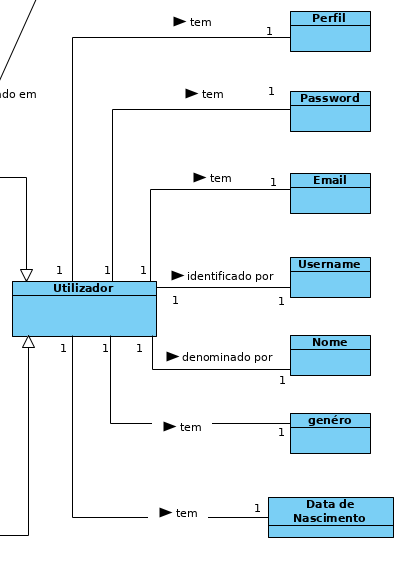
\includegraphics[scale=0.50]{images/modelação/utilizadores.png}
    \caption{Entidade Utilizador.}
    \label{fig:interfaceperfilptbycliente}
\end{figure}

\hspace{5mm} Tal como se pode observar a entidade \textbf{Utilizador} representa a informação comum a ambos os utilizadores, essa informação é: o \textbf{username} pelo qual o mesmo é identificado, o \textbf{nome} pelo qual é denominado, o \textbf{email} para pode ser contactado, a \textbf{password} que assegura a sua conta, o \textbf{género} e por última a sua \textbf{data de nascimento} (a partir da mesma pode ser derivada a sua idade). Juntamente com a informação referida e outras, específicas a cada utilizador (referidas adiante), o Utilizador contém um \textbf{perfil} que pode ser consultado por outros.

\hspace{5mm} Existem dois tipos de utilizadores: o \textbf{Cliente} e o \textbf{Personal Trainer}. De seguida seguinte encontra-se representado o Cliente.

\begin{figure}[H]
    \centering
    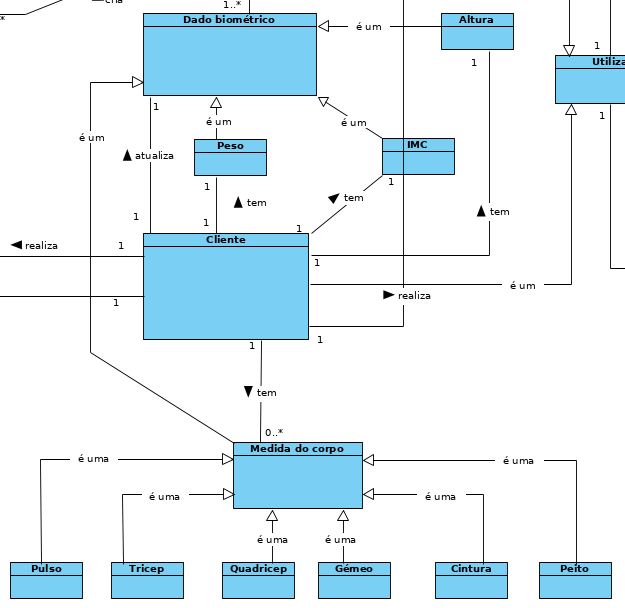
\includegraphics[scale=0.50]{images/modelação/cliente.png}
    \caption{Entidade Cliente.}
    \label{fig:interfaceperfilptbycliente}
\end{figure}

\hspace{5mm} O Cliente, a acrescentar à informação já referida, pode conter oito \textbf{dados biométricos}, sendo que as medidas: do \textbf{pulso, trícep, quadrícep, gémeo, cintura e peito} são dados opcionais, no entanto a introdução do \textbf{peso e altura} é obrigatória no momento de registo no sistema. O \textbf{IMC - Índice de Massa Corporal} - é derivado através de uma fórmula a partir do peso e altura sendo que as categorias (do IMC) que apresentamos no sistema seguem os dados fornecidos pela OMS - Organização Mundial de Saúde. Todos estes dados podem ser actualizados a qualquer momento e são sempre preservados os registos anteriores de modo a existir uma noção de histórico/ evolução. Note-se que apesar de opcionais, é recomendado a introdução de todos os dados uma vez que são métricas que permitem um acompanhamento mais personalizado e conclusivo sobre a evolução do plano de treino permitindo ajustar o plano consoante os resultados.

\hspace{5mm} O Personal Trainer é representado de seguida.

\begin{figure}[H]
    \centering
    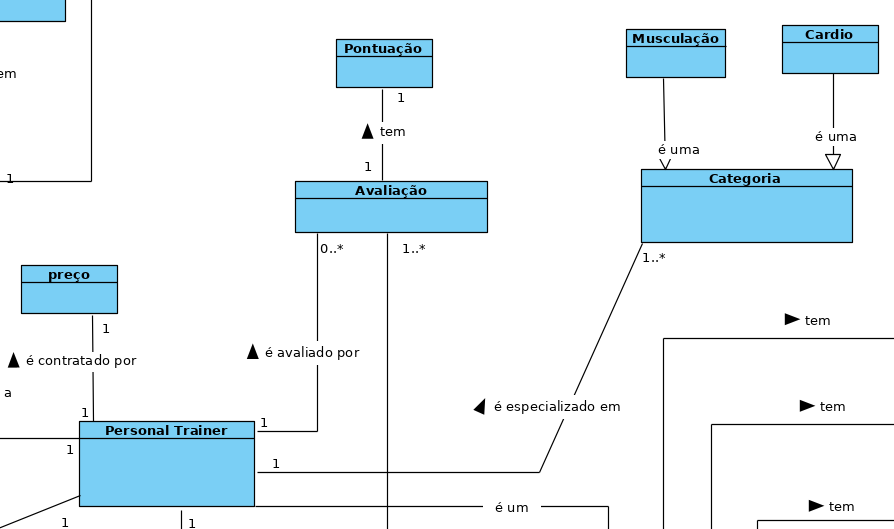
\includegraphics[scale=0.45]{images/modelação/pt.png}
    \caption{Entidade Personal Trainer.}
    \label{fig:interfaceperfilptbycliente}
\end{figure}

\hspace{5mm} Do mesmo modo, além da informação comum, contém também o \textbf{preço} que aplica ao Cliente por cada Workout (entidade explicada mais à frente), contém também a \textbf{categoria} em que é especializado, podendo ser em \textbf{musculação ou cardio}. Esta categoria pode ser útil quando o Cliente está a escolher o Personal Trainer que deseja ou mesmo pode ser útil ao próprio Personal Trainer para aceitar ou recusar um pedido de plano de treino uma vez que esse pedido pode não corresponder à sua categoria. A \textbf{avaliação} 
pode ser, também, decisiva no momento da escolha. Esta é realiza pelo Cliente uma única vez durante o plano de treino, numa escala de 1 a 5 estrelas (\textbf{pontuação}), sendo registada e associada às avaliações já existentes, calculando-se a média das mesmas.

\hspace{5mm} De seguida apresentam-se as entidades principais do modelo de negócio.

\begin{figure}[H]
    \centering
    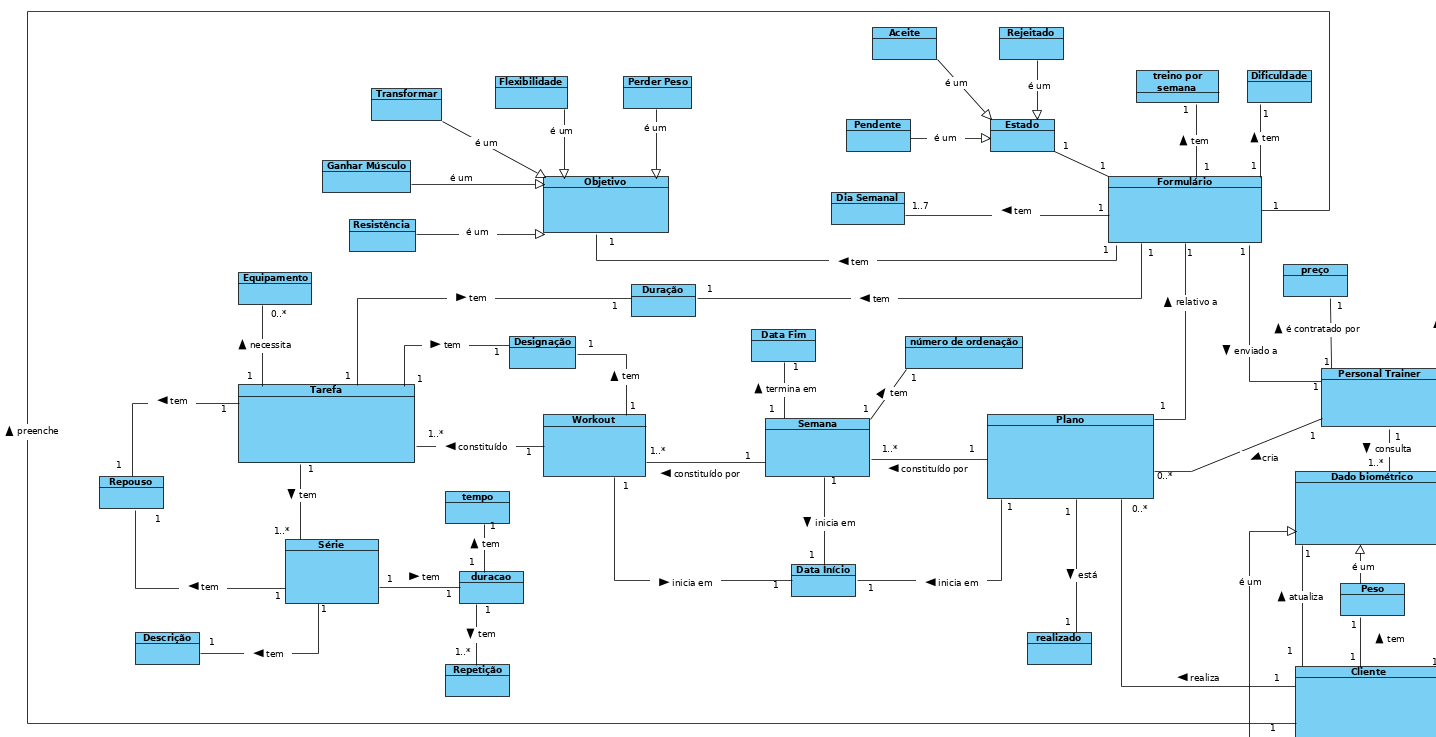
\includegraphics[scale=0.37]{images/modelação/core.png}
    \caption{Entidades principais do modelo de negócio.}
    \label{fig:interfaceperfilptbycliente}
\end{figure}

\hspace{5mm} Para iniciar um \textbf{plano} de treino, previamente, o Cliente tem de preencher um \textbf{formulário} onde indica a \textbf{dificuldade} que pode ser: \textbf{fácil, normal, difícil ou extrema}; é indicado também o número de \textbf{treinos semanais} juntamente com os \textbf{dias semanais} que tem disponibilidade, o \textbf{objectivo} que pode ser: \textbf{perder peso, ganhar músculo, resistência, flexibilidade e transformar gordura em massa magra}; e por último a \textbf{duração} em semanas.

\hspace{5mm} O formulário fica com o \textbf{estado pendente} até ao Personal Trainer o \textbf{rejeitar} ou \textbf{aceitar}. Caso o Personal Trainer aceite, imediatamente pode criar a primeira \textbf{semana} do \textbf{plano} de treino. 

\hspace{5mm} Uma semana ocorre entre duas datas: \textbf{data de início} e \textbf{data de fim}, contém também (internamente) o \textbf{número (de ordenação)} da semana no plano de treino. 

\hspace{5mm} A \textbf{semana} é constituída, também, por 1 ou mais \textbf{Workouts} que representa um dia de treino, por isso ocorre numa determinada \textbf{data} (num dia da semana), a \textbf{designação} que resume o treino nesse dia e a lista de \textbf{tarefas} a realizar.

\hspace{5mm} Uma \textbf{tarefa} contém, também, uma \textbf{designação}, uma \textbf{duração} (em minutos), pode necessitar de \textbf{equipamento} e as sucessivas tarefas são intervaladas por um \textbf{tempo de repouso}, por último é constituída por várias \textbf{séries}.

\hspace{5mm} A \textbf{série} é a unidade mais básica do plano de treino, contém uma \textbf{descrição} que indica a actividade a ser realizada. Tal como a tarefa, cada série é também intervalada com um \textbf{tempo de repouso}. Por último contém uma \textbf{duração} que pode ser em \textbf{tempo} (segundos ou minutos) ou em \textbf{número de repetições}. Para clarificar a noção de duração observe-se os seguintes exemplos: caso a série seja realizar 30 abdominais, a duração é 30 repetições, por outro lado, caso a série seja realizar a o movimento de prancha durante 1 minuto, a duração é em tempo (neste caso em minutos). 
\chapter{Arquictetura}
\label{chap:arquitetura}

\hspace{5mm} Na elaboração da arquitectura o primeiro passo foi definir as entidades em termos de classes do sistema, maior parte já detectadas no modelo de domínio. Durante esta fase o grupo apercebeu-se que fazia sentido dividir as entidades em dois grupos que se traduzem em dois subsistemas: os \textbf{Recursos Humanos} e o \textbf{Core}. Note-se que estes sub-sistemas a nível de implementação traduzem-se em dois packages.

\hspace{5mm} Os recursos humanos contém as classes que representam os utilizadores do sistema, ou seja, o cliente e personal trainer.

\hspace{5mm} No entanto após alguma pesquisa e discussão de ideias entre o grupo, percebeu-se que na actualidade as aplicações webs ou outras são orientadas a serviços.

\section{Arquitetura orientada a serviços}

\hspace{5mm} Desta forma, a ideia inicial foi separar os dois packages definidos anteriormente o \textbf{core} e os \textbf{recursos humanos}, bem como o frontend, sendo já uma boa arquitectura. No entanto, percebeu-se que que poderia ser mais bem dividido, para se tirar melhor partido, dessa forma chegou-se aos sete serviços:

\begin{itemize}
    \item Core: responsável pelas funcionalidades que interagem com planos.
    \item Requests: responsável pelas funcionalidades que interagem com os pedidos/formulários.
    \item Notifications: responsável pelas funcionalidades que interagem com as notificações.
    \item Clients: responsável pelas funcionalidades que interagem com os clientes.
    \item PersonalTrainers: responsável pelas funcionalidades que interagem com os PTs.
    \item GymAtHome: API do backend, ou seja, dispathcer dos pedidos para os serviços correctos.
\end{itemize}

\hspace{5mm} A tomada desta decisão passou por uma verificação das vantagens e desvantagens do desenvolvimento deste tipo de arquitecturas.

\hspace{5mm} As \textbf{vantagens} de desenvolver um arquitectura orientada a serviços são as seguintes:
\begin{itemize}
    \item divisão de trabalho mais fácil, aumentando assim a produtividade.
    \item divisão de responsabilidades.
    \item são mais contidos, dessa forma, mais fácil encontrar erros, bem como fazer deployment.
    \item permitem escalabilidade da arquitectura para aumento de carga.
    \item a falha de serviços não provoca directamente a falha do sistema, isto é, resiliência.
    \item quando são feitas alterações ao código, apenas necessita-se de fazer deployment do serviço alterado, não precisando de esperar por outros serviços, ou seja, deployment contínuo.
    \item permitem mais flexibilidade da arquitectura.
    \item ...
\end{itemize}

\hspace{5mm} As \textbf{desvantagens/falácias} cometidas quando de desenvolve orientado a serviços:
\begin{itemize}
    \item pensar que a banda larga é infinita.
    \item pensar que não existe latência.
    \item pensar que os dispositivos de rede são uniformes.
    \item pensar que não existem hackers.
    \item necessidade de mais recursos.
    \item ...
\end{itemize}

\hspace{5mm} No entanto, apesar de conter-se algumas desvantagens, as vantagens sobrepõem-se, obtendo-se melhores resultados a nível de escalabilidade com uma arquitectura orientada a serviços.

\hspace{5mm} Na verdade, "nem tudo é um mar de rosas", ao desenvolver uma arquitectura orientada a serviços, acresce uma complexidade, que consiste em manter serviços consistentes, pois alguns depende dos dados de outros, como por exemplos os outros serviços dependem do clientes e personal trainers, pois quando existe o registo dos mesmos, tem-se que propagar essa \textbf{escrita} para todos os serviços. No entanto, mais uma vez, esta complexidade extra em alguns serviços, não sobrepõe as vantagens.

\hspace{5mm} Outro problema encontrado nesta arquitectura foi a necessidade mais recursos de CPU e RAM do que o costume. No entanto em produção não seria problema, visto que seriam disponibilizados mais recursos. 

\hspace{5mm} De seguida, serão apresentadas as várias decisões, tomadas na arquitectura, bem como a apresentação dos serviços individualmente.

\section{Client Service}

\hspace{5mm} O package HRClient (HR alusivo a Human Resource) encontra-se especificado nas seguintes figuras.

\begin{figure}[H]
    \centering
    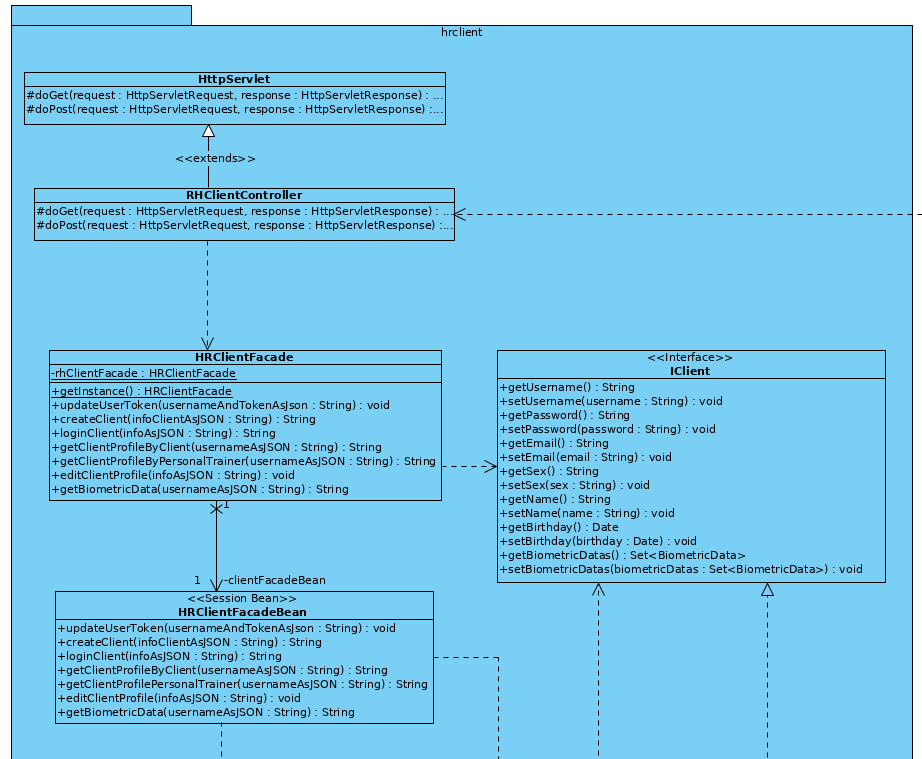
\includegraphics[scale=0.575]{images/arquitetura/client-package-1.png}
    \caption{Diagrama de classes do package HRClient - parte 1.}
    \label{fig:interfaceperfilptbycliente}
\end{figure}


\begin{figure}[H]
    \centering
    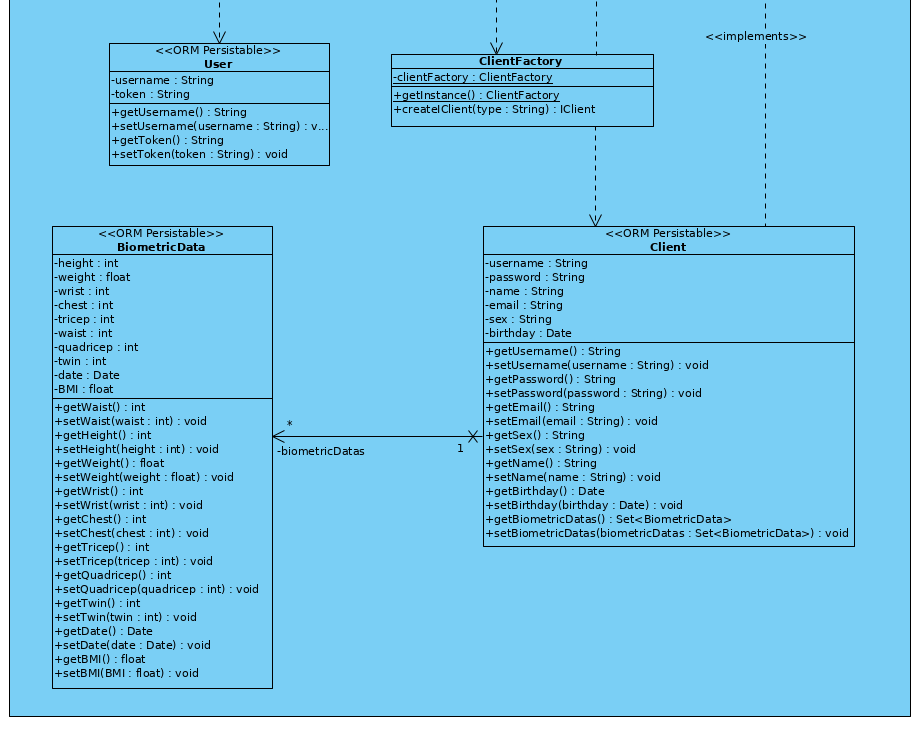
\includegraphics[scale=0.575]{images/arquitetura/client-package-2.png}
    \caption{Diagrama de classes do package HRClient - parte 2.}
    \label{fig:interfaceperfilptbycliente}
\end{figure}


\hspace{5mm} Em relação ao cliente foi criada a classe \textbf{Client} com a informação específica do mesmo, tal como referido anteriormente no modelo de domínio, o cliente contém um histórico de dados biométricos, para isso foi criada uma associação entre a classe Client e a classe \textbf{BiometricData}. \textbf{Note-se que a relação é de um para muitos uma vez que existe a noção de histórico} apesar de não estar implementada a funcionalidade de visualização do mesmo a na UI. De seguida foi introduzida a interface \textbf{IClient} de forma a que as classes que utilizam a mesma \textbf{dependam apenas da interface e não da classe concreta}. Esta prática \textbf{facilita a evolução e manutenção do código} pois caso, no futuro, sejam introduzidas novas classes concretas que representam clientes (ex: ClientPremium, etc) desde que as mesmas implementem o tipo IClient, o código continuará a funcionar sem alterações. 

\subsection{Factory Method}

\hspace{5mm} Com o mesmo objectivo, para facilitar a evolução e manutenção do código, foi introduzido o \href{https://refactoring.guru/design-patterns/what-is-pattern}{design pattern} \href{https://refactoring.guru/design-patterns/factory-method}{Factory Method} que é responsável pela criação dos clientes. Para tal foi criada a classe \textbf{Factory Method}. A grande vantagem da utilização deste design pattern é que o processo de criação/ instanciação do objecto do tipo IClient passa a ser responsabilidade da classe ClientFactory, desta forma as classes que utilizam o IClient em vez de dependerem dos tipos concretos (uma vez que antes as próprias faziam a instanciação do objecto) passam a depender apenas da interface IClient e da classe ClientFactory. \textbf{Analisando a arquitectura actual, pode parecer que não houve vantagem na introdução do Factory Method uma vez que antes existiam 2 dependências, com a interface IClient e a classe Client e após a introdução do mesmo continuam a existir o mesmo número de dependências, neste caso com a interface IClient e classe ClientFactory. No entanto, numa perspectiva evolutiva e pensando no futuro, caso sejam introduzidas N classes do tipo IClient, as dependências são reduzidas de N+1 (N classes + interface IClient) para 2 apenas (ClientFactory + IClient)} por este motivo o grupo entendeu que se justifica a introdução do Factory Method.

\hspace{5mm} Note-se que apesar do design pattern referido anteriormente ter sido introduzido na proposta inicial da arquitectura, após gerado o código, na prática acabou por não ter sido implementado pelo grupo uma vez que foi utilizada a API \href{https://github.com/google/gson}{gson}, desenvolvida pela Google, responsável pela serialização e deserialização de objectos Java para o formato \href{https://en.wikipedia.org/wiki/JSON}{JSON}. Esta API internamente já implementa o Factory Method por isso não foi necessário uma implementação concreta pelo grupo. No entanto a classe ClientFactory permanece no código, apesar de não implementada, para que, caso, no futuro, seja necessária a sua utilização, a arquitectura já conte com a mesma. Para clarificar, uma possível hipótese de necessidade de utilizar a própria implementação por parte do grupo seria por exemplo, caso a API gson fosse descontinuada. 

\subsection{Adpater}

Ainda devido à utilização da API referida anteriormente foi necessária a introdução do design pattern \href{https://refactoring.guru/design-patterns/adapter}{Adapter} uma vez que a API apenas consegue serializar/deserializar certos tipos de objectos conhecidos (int, boolean, String, List, Array, Date, etc) por isso para serializar/deserializar um Client visto que tem uma relação com a classe BiometricData é necessário indicar como essa serialização/deserialização deve ser feita, sendo a mesma através de classes auxiliares como a \textbf{BiometricDataSerializer} que se comporta como um adaptador do tipo BiometricData.

\subsection{Hibernate}

\hspace{5mm} Tanto as classes User (mais á frente explicada), Client como BiometricData foram identificadas como \textbf{ORM Persistable} uma vez que se pretende persistir a informação das mesmas. Para tal utilizou-se a framework \href{https://hibernate.org/}{Hibernate} integrada como plugin (built-in) na ferramenta \href{https://www.visual-paradigm.com/}{Visual Paradigm} de modo a automatizar a criação das classes \href{https://www.tutorialspoint.com/design_pattern/data_access_object_pattern.htm}{DAO} que são responsáveis por realizar operações CRUD  (entre outras interrogações) sobre os objectos persistidos. Para tal a framework hiberante fornece \textbf{mapeamento automático (ou de fácil configuração) das classes (neste caso Java) para tabelas numa base de dados relacional} (neste caso MySQL) através da sinalização no diagrama de classes ou anotações no código gerado. Ainda fornece \textbf{abstracção da tecnologia de conexão à base de dados, inclusive gestão de sessões}, podendo, por isso, ser configurada para diferentes base de dados, \textbf{sem alteração do código}. No entanto tem a desvantagem de existir um acréscimo computacional no uso da framework, ainda assim analisando as vantagens oferecidas compensa a utilização da mesma.

\subsection{EJB}

\hspace{5mm} Foi criada também a classe \textbf{HRClientFacadeBean} que implementa uma \textbf{Session Bean Stateless} onde as operações a realizar são definidas. A utilização dos EJB fornece a gestão automática de \textbf{sincronização das interacções entre objectos em ambiente concorrente}, gestão da \textbf{partilha de recursos/ objectos entre componentes ou intervenientes no sistema}, por exemplo na partilha das sessões na conexão à base de dados, utiliza a \textbf{JNDI} que é uma API de lookup que permite a \textbf{procura de recursos (procura da referência do recurso) através de um nome previamente atribuído a esse mesmo recurso}, fornece também \textbf{interoperabilidade}, por exemplo através de protocolos como o \textbf{WSDL}, apesar do grupo não ter utilizado neste projecto, uma vez que foi utilizado o protocolo \textbf{REST} para comunicação entre serviços que será detalhado mais à frente, a utilização de EJBs disponibiliza outras funcionalidades não referidas. Em suma, o grupo entendeu que a utilização de EJBs é vantajosa uma vez se adequa ao contexto de utilização do sistema pois existem:

\begin{itemize}
    \item muitos utilizadores, isto é, muitas instâncias de aplicações cliente;
    \item milhares de objectos criados e em utilização;
    \item muitas interacções entre os objectos;
    \item concorrência e operações com requisitos transaccionais.
\end{itemize}

\subsection{Multi-camada e Facade}

\hspace{5mm} De forma a implementar o \href{https://en.wikipedia.org/wiki/Architectural_pattern#:~:text=An\%20architectural\%20pattern\%20is\%20a,minimization\%20of\%20a\%20business\%20risk.}{padrão arquitectural} denominado por \href{https://en.wikipedia.org/wiki/Multitier_architecture}{multi camada} foi implementado o design pattern \href{https://refactoring.guru/design-patterns/facade}{Facade} que expõe a \textbf{API} do serviço contido nesse package de modo a que \textbf{as classes contidas nos packages exteriores apenas comuniquem com as classes internas a este package através de um único ponto}, neste caso a classe \textbf{HRClientFacade}, reduzindo assim o número de dependências entre os packages. Para se entender a vantagem deste design pattern, segue-se um exemplo: caso o package business apenas comunique com o package data através do DataFacade, se a implementação interna do package data muda-se drasticamente, \textbf{o package business não sofria qualquer alteração} desde que a classe DataFacade continuasse a existir e mantive-se os protótipos dos seus métodos inalterados, isto é, a sua API inalterada.

\subsection{Singleton}

\hspace{5mm} Ainda neste package, visto que ambas as classes ClientFactory e HRClientFacade devem ter um única instância em todo o sistema foi implementado o design pattern \href{https://refactoring.guru/design-patterns/singleton}{Singleton}.

\subsection{REST vs WSDL}

\hspace{5mm} De forma a tornar a funcionalidade fornecida por este package \textbf{facilmente acessível por qualquer outro serviço ou sistema} foi implementado um servidor utilizando Java Servlets contidos na API Java EE, na qual a classe que implementa o Servlet, neste caso denominada por \textbf{HRClientController}, responde a pedidos recebidos através do protocolo \textbf{HTTP}. O grupo decidiu utilizar o protocolo REST ao invés de WSDL para a comunicação entre serviços uma vez que a complexidade de cada serviço é relativamente reduzida (consequência directa da divisão do sistema em serviços menos complexos), outra razão é o facto de existir total conhecimento no contexto de utilização e conteúdo transmitido nos pedidos HTTP, por 
último visto que na componente frontend, algumas funcionalidades são acedidas por \textbf{AJAX}, a utilização de REST torna-se mais adequada. 


\subsection{Token Authentication}

\hspace{5mm} Observando o diagrama de classes deste package existe uma classe ainda não abordada, a classe \textbf{User}. Esta classe foi criada unicamente para implementar um método de autenticação do utilizador, quer seja um cliente ou personal trainer, na evocação externa de qualquer método. Desta forma no momento de \textbf{registo} ou \textbf{login} de qualquer utilizador no sistema é gerado um \textbf{token único e aleatório} armazenado no sistema numa instância da classe User e retornado ao utilizador para que seja também armazenado temporariamente na aplicação client-side, assim numa futura evocação de qualquer método o token é verificado e caso coincide é permitida a interacção do utilizador.


\section{Personal Trainer Service}

\hspace{5mm} O package HRPersonalTrainer encontra-se especificado nas seguintes figuras.

\begin{figure}[H]
    \centering
    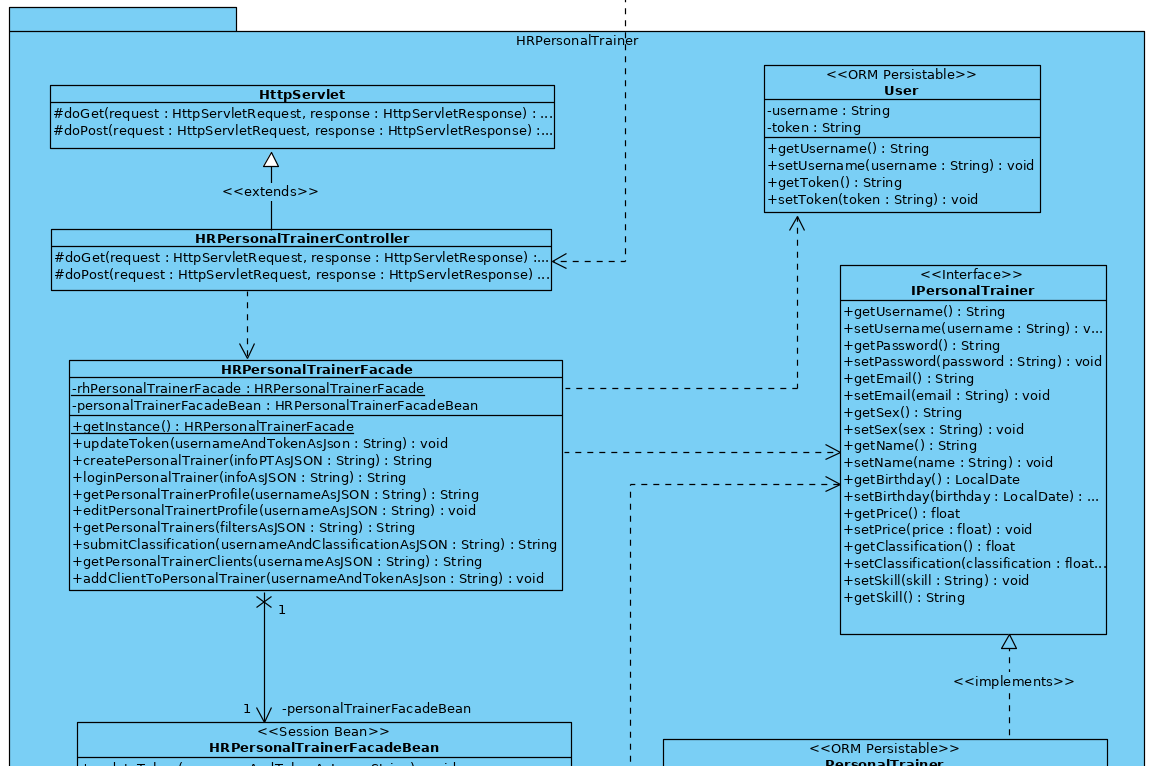
\includegraphics[scale=0.45]{images/arquitetura/pt-package-1.png}
    \caption{Diagrama de classes do package HRPersonalTrainer - parte 1.}
    \label{fig:interfaceperfilptbycliente}
\end{figure}


\begin{figure}[H]
    \centering
    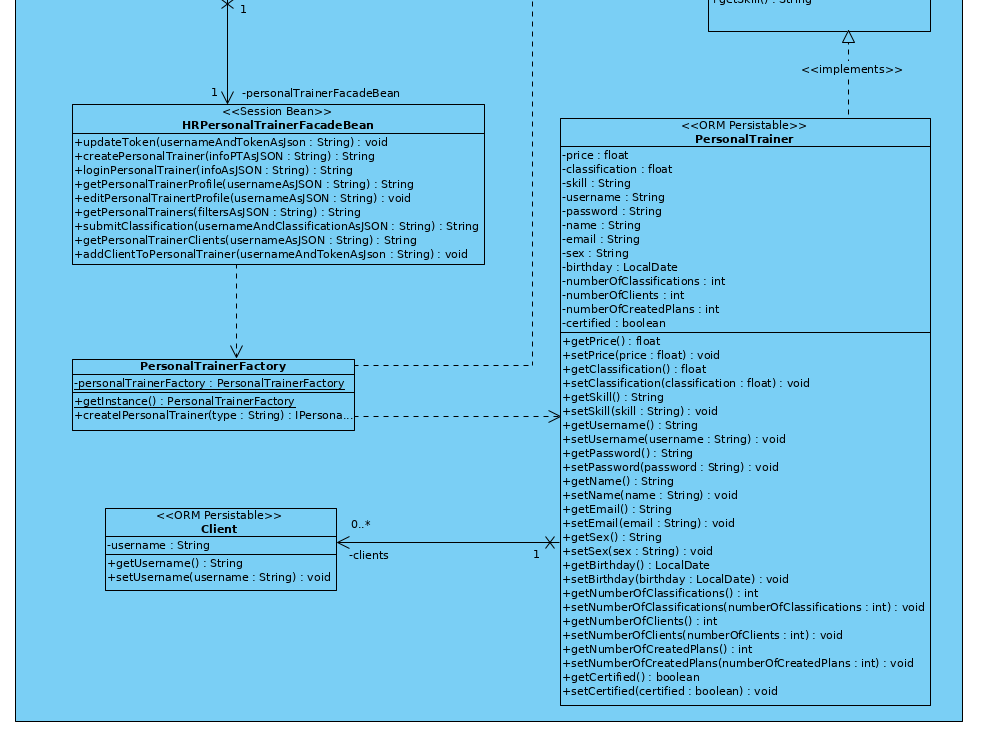
\includegraphics[scale=0.5]{images/arquitetura/pt-package-2.png}
    \caption{Diagrama de classes do package HRPersonalTrainer - parte 2.}
    \label{fig:interfaceperfilptbycliente}
\end{figure}

\hspace{5mm} Analogamente ao Client Service e pelos mesmos motivos no package HRPersonalTrainer foram implementados os design pattern: \textbf{FactoryMethod, Adapter, Singleton e Facade}. A lógica de negócios foi, também, implementada num \textbf{Session Bean} e o serviço exposto através do protocolo \textbf{REST} utilizando \textbf{autenticação por tokens}.

\hspace{5mm} No entanto foi necessária a associação entre um cliente e um personal trainer para isso foi introduzida a classe \textbf{Client} também esta persistida.

\section{Core}

\hspace{5mm} O package Core encontra-se especificado nas seguintes figuras.

\begin{figure}[H]
    \centering
    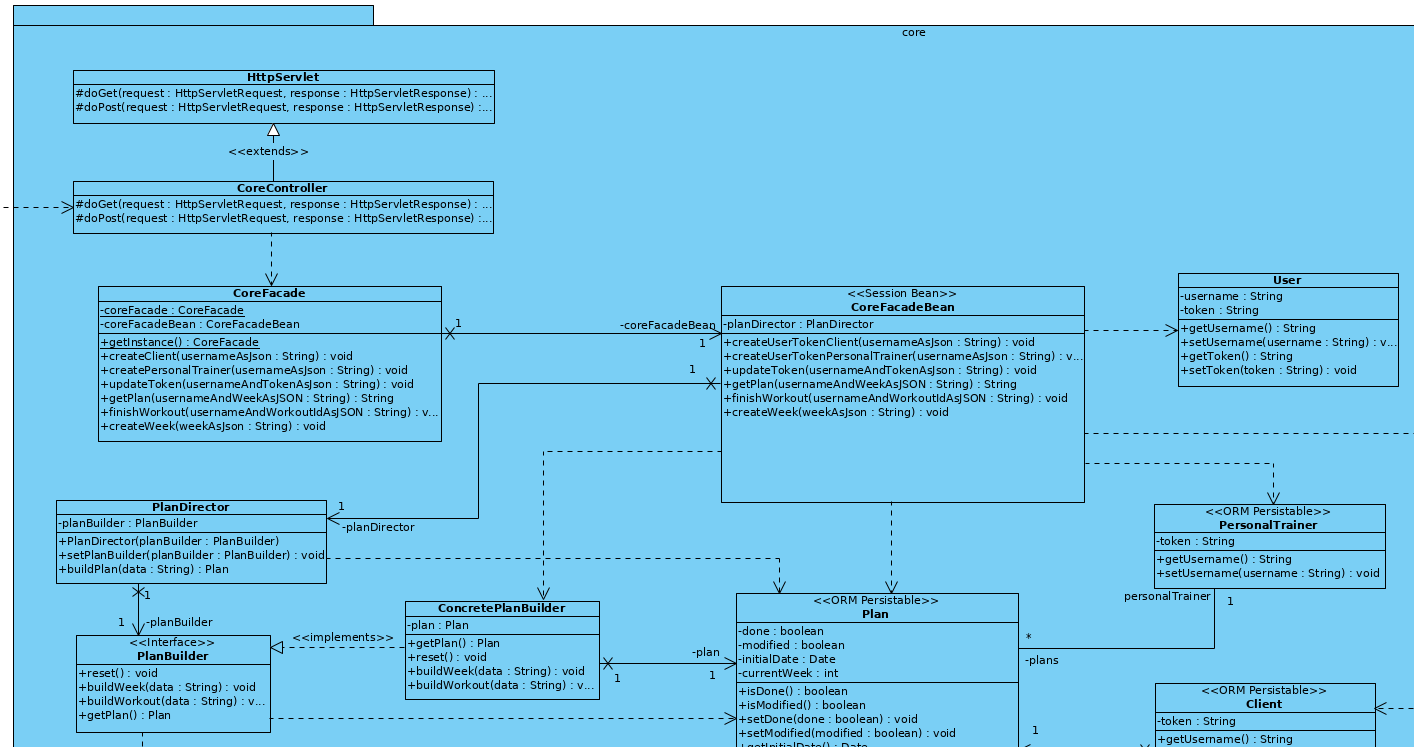
\includegraphics[scale=0.35]{images/arquitetura/core-package-1.png}
    \caption{Diagrama de classes do package Core - parte 1.}
    \label{fig:interfaceperfilptbycliente}
\end{figure}


\begin{figure}[H]
    \centering
    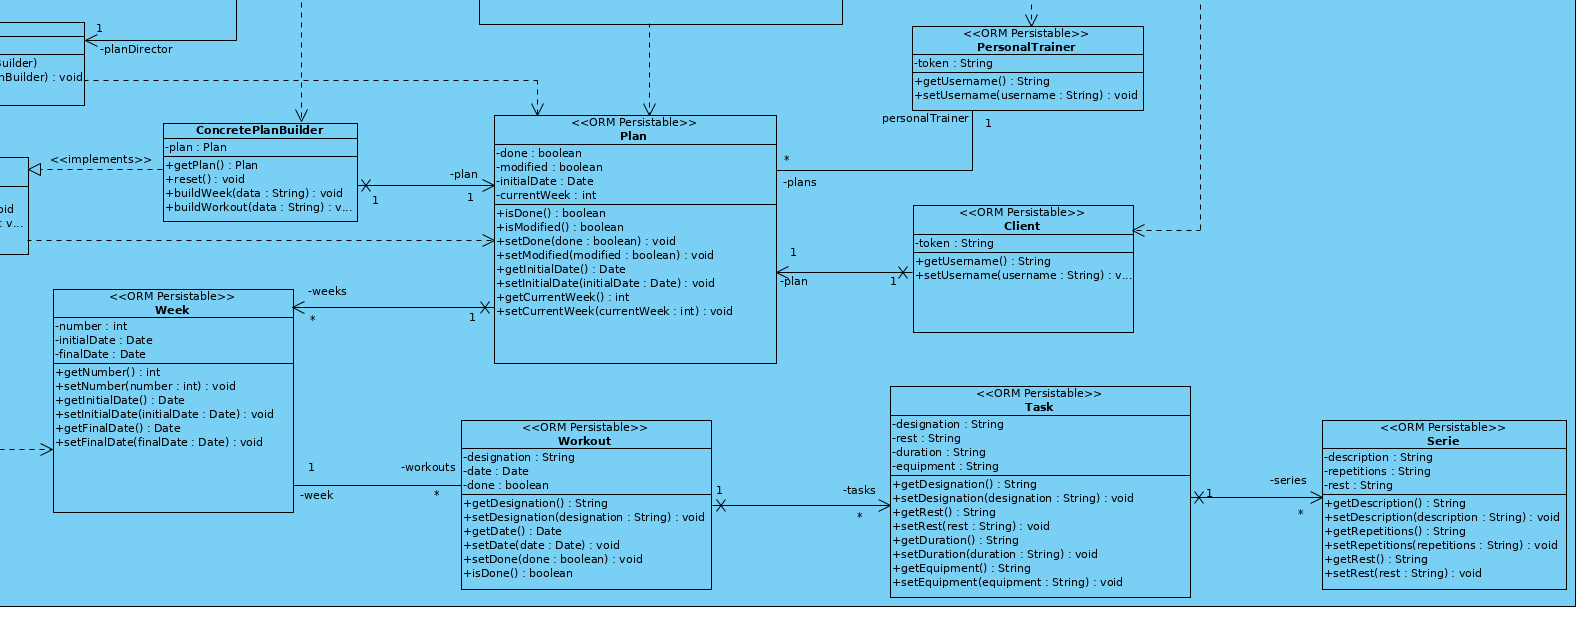
\includegraphics[scale=0.325]{images/arquitetura/core-package-2.png}
    \caption{Diagrama de classes do package Core - parte 2.}
    \label{fig:interfaceperfilptbycliente}
\end{figure}

\hspace{5mm} O Core contém as entidades principais do modelo de negócio, no contexto deste projecto, contém as classes: \textbf{Plan}, \textbf{Week}, \textbf{Workout}, \textbf{Task} e \textbf{Serie}; já descritas anteriormente no modelo de domínio.

\hspace{5mm} Analogamente aos serviços anteriores e pelos mesmos motivos no package Core foram implementados os design pattern: \textbf{Adapter, Singleton e Facade}. A lógica de negócios foi, também, implementada num \textbf{Session Bean} e o serviço exposto através do protocolo \textbf{REST} utilizando \textbf{autenticação por tokens}.

\hspace{5mm} Note-se na relação entre certas classes foi vantajoso utilizar a dupla navegabilidade uma vez que o dupla direcção no acesso entre ambos os objectos é útil. 

\subsection{Método finishWorkout}

\hspace{5mm} O método \textbf{finishWorkout()} responsável por finalizar um determinado Workout tem elevada relevância no sistema. Não só realiza a operação evidente de Update (neste caso actulização do estado do workout para realizado), mas também tem uma funcionalidade adicional tal como, avançar automaticamente a semana do plano em que o cliente se encontra caso todos os workouts dessa semana tenham sido realizados. Para clarificar segue-se um exemplo, caso por exemplo o Plano de treino do Cliente se encontre na semana 3 (semana actual), mas se este realizar todos os workouts da semana 5 a sua semana actual passa a ser a 6, este sistema de actualização da semana actual foi baseado em outras aplicações, tal como a Netflix, em que se um utilizador estiver na temporada 3, mas depois for ver um episódio da temporada 5, quando voltar a entre no site para voltar a ver a série será remetido automaticamente para a temporada 5.

\subsection{Builder}

\hspace{5mm} No Core foi implementado o Design Pattern Builder, este é um Pattern criacional, no qual os principais objectivos é reduzir o número de dependências, pois todos as classes apenas ficam dependentes do PlanDirector, sendo este o único a ter as dependências necessárias. Outro objectivo é a criação do objecto por passos.

\hspace{5mm} Tal como nos serviços Client e PT o este design pattern acabou por não ser implementado em código porque a biblioteca GSON consegue ela própria criar o objecto todo através de um json e das classes de Deserialização criadas.

\section{Requests Service}

\hspace{5mm} Analogamente ao serviços anteriores e pelos mesmos motivos no package Requests foram implementados os design pattern: \textbf{Singleton e Facade}. A lógica de negócios foi, também, implementada num \textbf{Session Bean} e o serviço exposto através do protocolo \textbf{REST} utilizando \textbf{autenticação por tokens}.

\hspace{5mm} O serviço Requests tal como o nome sugere é um serviço que guarda informações sobre pedidos, pedidos estes submetidos por Clientes para os PTs, nos quais consta informação sobre o tipo de Plano que desejam realizar. O Cliente tem acesso a todos os pedidos que realizou, por outro lado o PT só tem acesso aos pedidos que ainda tem pendentes.

\hspace{5mm} Os Pts podem aceitar ou rejeitar pedidos sempre essa informação ilustrada aos Clientes, pois o aceitar ou rejeitar de um pedido altera o seu estado.

\begin{figure}[H]
    \centering
    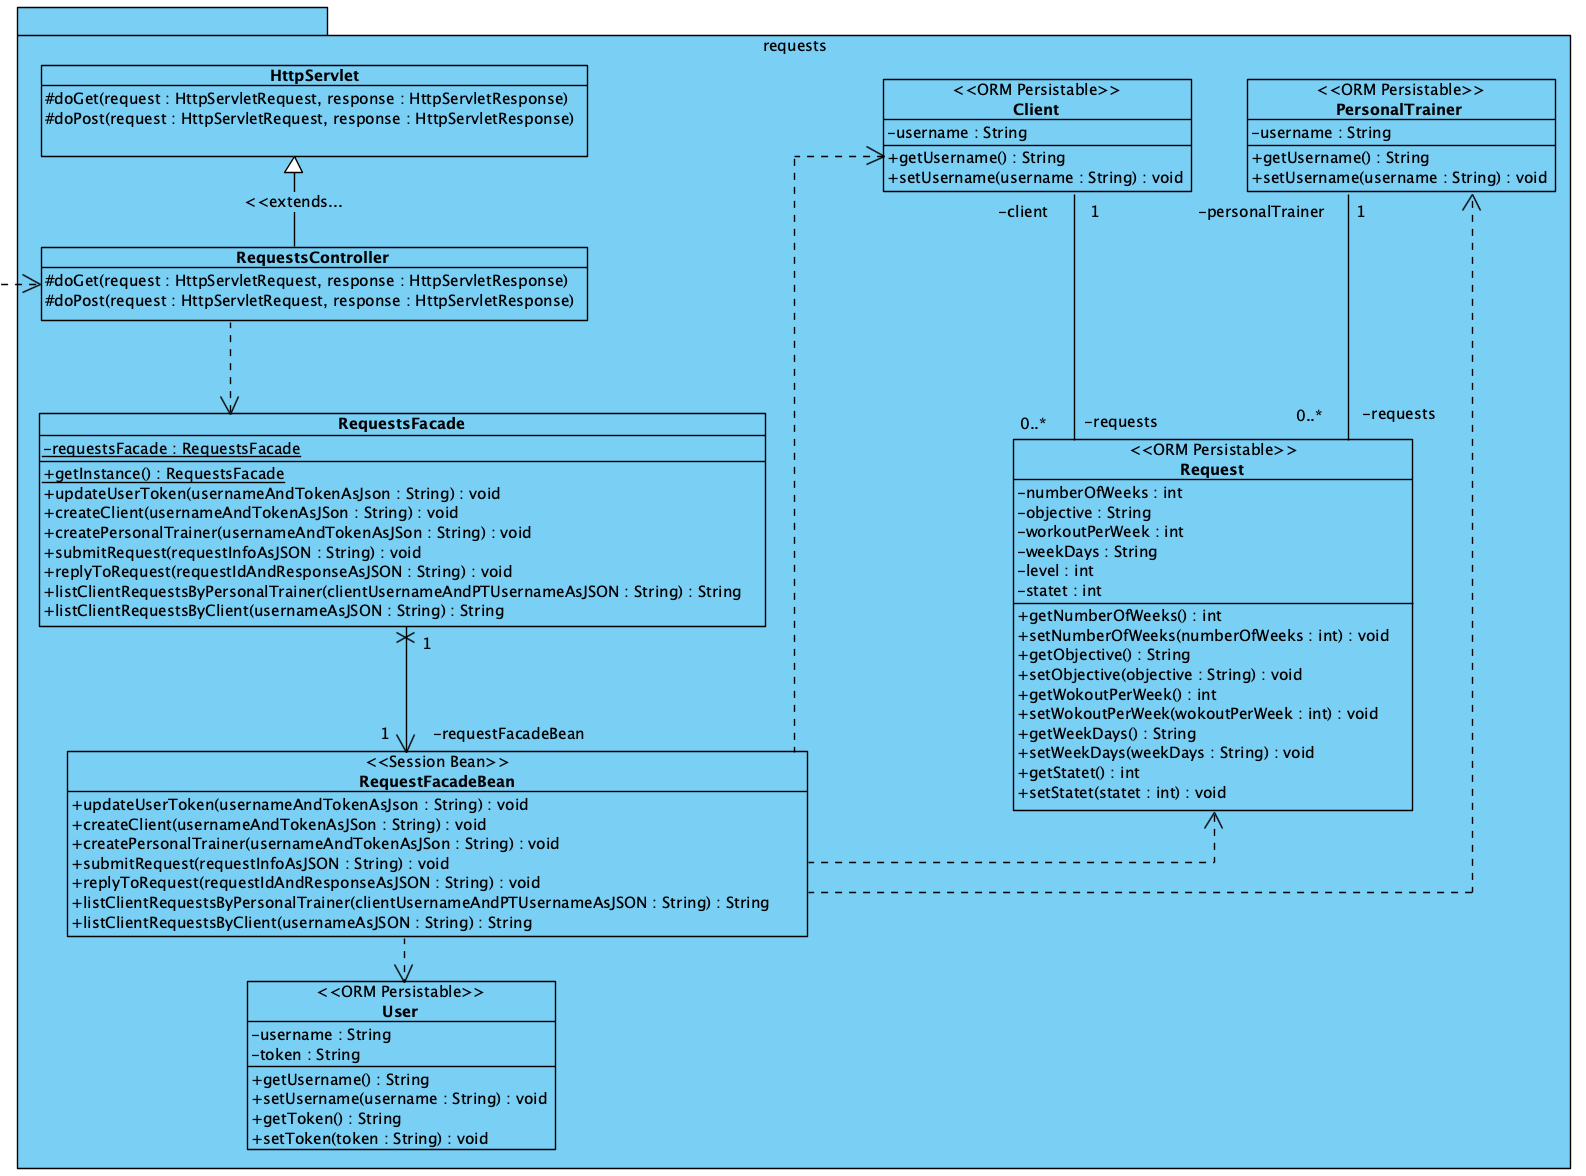
\includegraphics[scale=0.5]{images/arquitetura/requests-package.png}
    \caption{Diagrama de classes do package Notification}
    \label{fig:my_label}
\end{figure}

\section{Notifications Service}

\hspace{5mm} Analogamente ao serviços anteriores e pelos mesmos motivos no package Notifications foram implementados os design pattern: \textbf{Singleton e Facade}. A lógica de negócios foi, também, implementada num \textbf{Session Bean} e o serviço exposto através do protocolo \textbf{REST} utilizando \textbf{autenticação por tokens}.

\hspace{5mm} O serviço Notifications tal como o nome sugere é um serviço que guarda as notificações geradas pelo sistema para os utilizadores. O sistema apenas gera notificações consoante acções de utilizadores, estes quando realizam uma acção relacionada com outro o sistema irá criar uma notificação para o outro utilizador, de forma a que esta possa ser informado de alterações que existiram no sistema.

\hspace{5mm} Tanto os Clientes como os PTs podem marcar as notificações como lidas, desta forma será mais fácil numa próxima vista das notificações distinguir daquelas que estão por ler e as que já estão lidas.

\begin{figure}[H]
    \centering
    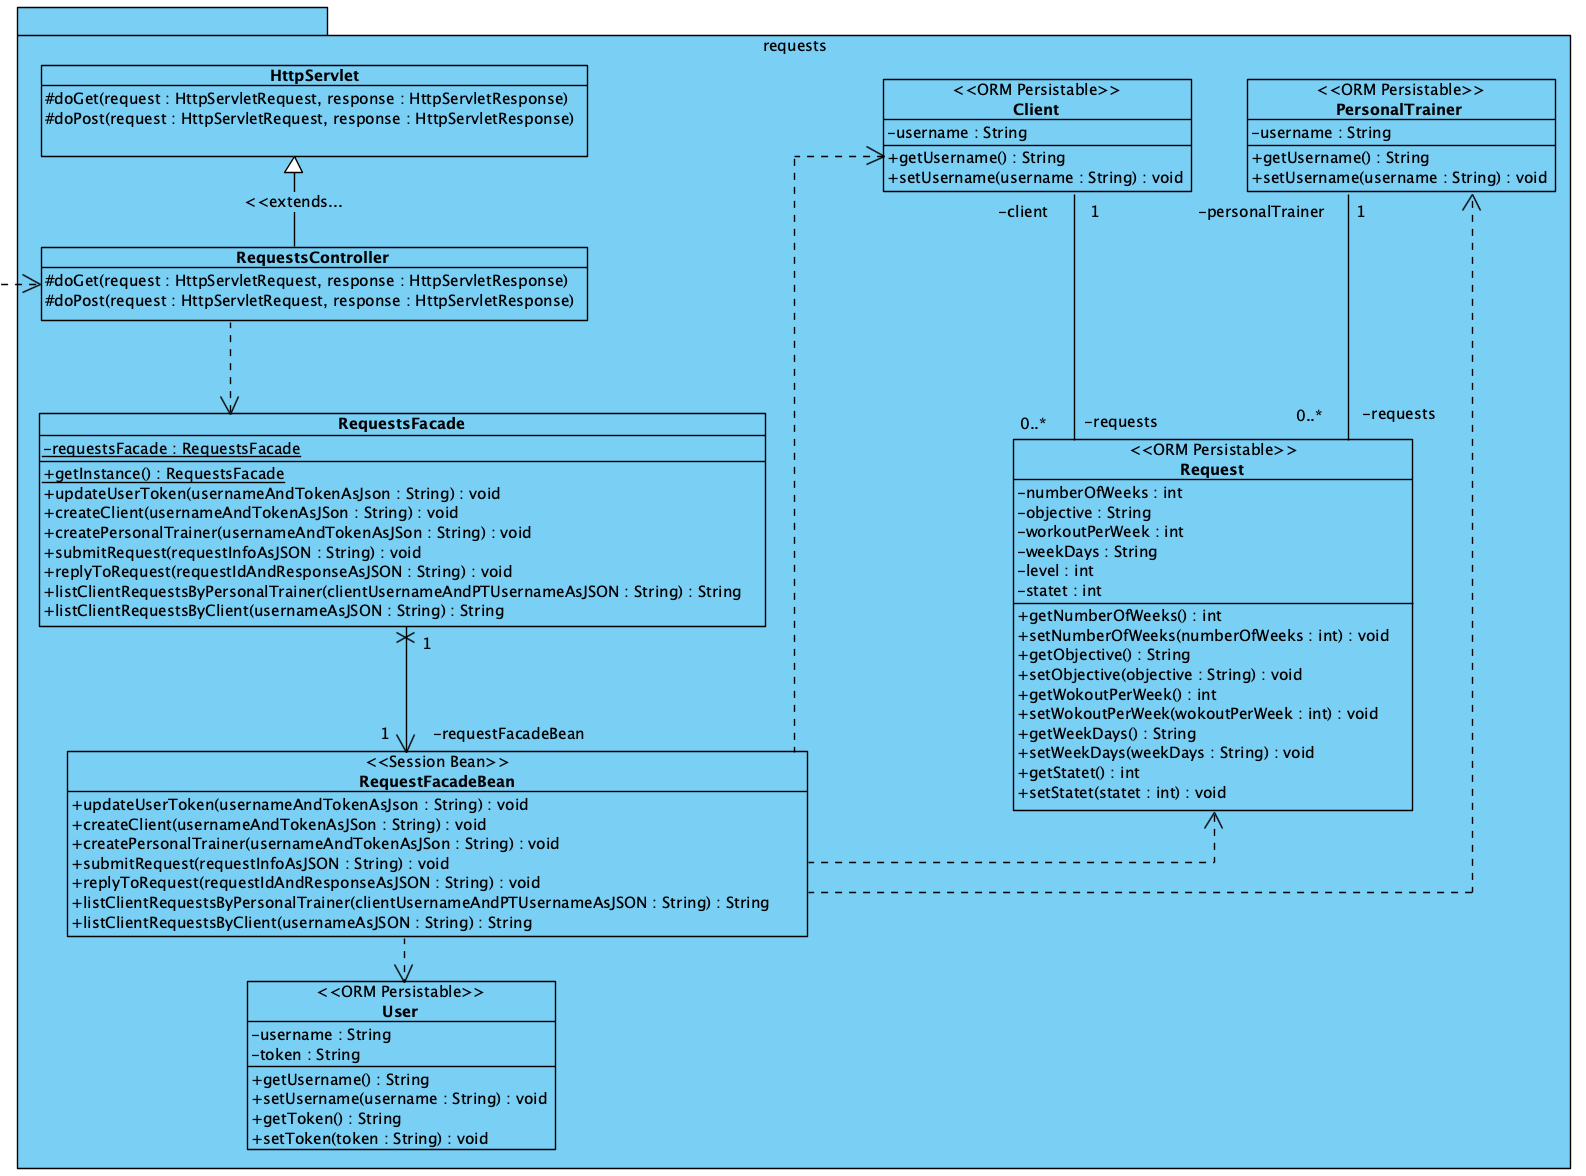
\includegraphics[scale=0.5]{images/arquitetura/requests-package.png}
    \caption{Diagrama de classes do package Request}
    \label{fig:my_label}
\end{figure}

\section{GymAtHome Service}

\subsection{Propagação dos tokens}

\hspace{5mm} Tal como referido anteriormente todos os serviços contêm um método de autenticação da interacção do utilizador através de um token gerado no login ou registo. Desta forma para que todos os serviços tenham todos os tokens mais actuais de cada cliente, este serviço principal (GymAtHome) tem a responsabilidade de propagar os tokens para os respectivos serviços externos, para isso foi definido o método updateToken nos mesmos.

\hspace{5mm} Este serviço serviço tem ainda o objectivo de criar notificações para os utilizadores, à medida que os utilizadores realizam certas acções podem ser geradas algumas notificações.

\hspace{5mm} A principal função deste serviço é servir de dispatcher, pois todos os pedidos enviados pelo \href{sec:frontend}{Frontend} são direccionados a este e este é que trata de encaminhar para o serviço correcto e de apenas reencaminhar a resposta do serviço que comunicou. Com os isto os outros serviços estão mais protegidos uma vez que o único ponto de acesso destes é através deste serviço.

\section{Frontend service}
\label{sec:frontend}

\subsection{MVC - Model View Controller}

\hspace{5mm} Para a comunicação entre os \textbf{Controllers} e respectivas páginas de apresentação (\textbf{Views}) foi implementado o padrão arquitectural \href{https://en.wikipedia.org/wiki/Model\%E2\%80\%93view\%E2\%80\%93controller}{MVC}. O acesso ao \textbf{Model} (que contem a lógica de negócio), por parte do Controller é realizado através do protocolo REST. A utilização deste padrão arquitectural, novamente, torna a evolução e manutenção do código facilitada uma vez que, por exemplo, caso o pacakage presentation (que contém os Controllers e respectivas Views) seja alterado, por exemplo, ao implementar uma nova UI para o sistema operativo Android ou IOS, visto que toda a lógica de negócio está unicamente contida no Model, o sistema (na componente backend) continuará totalmente funcional e inalterado.
\chapter{Usabilidade}
\label{chap:usabilidade}

\hspace{5mm} Nesta secção discute-se a importância da usabilidade no desenvolvimento deste projecto, os princípios que se podem encontrar, e em que medida os mesmos trazem melhorias para a interacção com o sistema.

\section{Conhecer os utilizadores}

\hspace{5mm} Um do grandes sábios de sistemas interactivos, \href{https://www.goodreads.com/quotes/8740235-we-must-design-for-the-way-people-behave-not-for}{Donald A. Normal} disse a seguinte afirmação, \textit{"We must design for the way people behave, not for how we would wish them to behave.”}, isto significa que, para desenvolver um bom sistema interactivo deve-se seguir a ideologia de que \textbf{o programa é feito para o utilizador}. Desta forma, deve-se desenvolver os programa a pensar nas necessidades do utilizador e como o mesmo pretende \textbf{usar} (usabilidade) o sistema de forma eficiente, eficaz e satisfatória, para atingir os seus objectivos. De forma muito resumida, deve-se desenvolver/desenhar focado na usabilidade. Por este motivo, neste projecto aplicou-se a mesma ideologia, ou seja, necessita-se de conhecer os utilizadores do programa.

\hspace{5mm} O conhecimento/análise dos utilizadores contém diversas técnicas conhecidas tais como: entrevista, observação, personas, etc. No entanto, face aos recursos que a equipa tem, a forma mais eficaz de conhecer o utilizador foi através de pesquisa e estudo do domínio do problema (exercício físico/ ginásio). Na verdade, começou-se por perceber a linguagem utilizada no meio, isto é, termos como: planos de treino, workouts, series, tempos entre series, personal trainer, entre outros. Apesar de poder parecer pouco importante, isto permitiu desenvolver uma interface com uma linguagem adequada aos utilizadores. Do mesmo modo, a utilização de interfaces simplistas, como se verá mais adiante também foi pensada no utilizador, pois pessoas focadas no exercício tendem a ser simplistas. Outra razão deve-se ao facto de a tendência actual de desenvolvimento web seguir a simplicidade das interfaces (seguir as \textbf{tendências}/\textbf{padrão} torna-se muito importante para se ter uma interface \textbf{consistente} com a actualidade).


\section{Princípios de usabilidade}

\hspace{5mm} Poder-se-á dizer que o desenvolvimento de interfaces torna-se uma processo consistente, desta forma, foram definidos/partilhados, princípios de usabilidade. Pode-se dizer que os princípios de usabilidade são regras/normas que guiam os desenvolvedores/designers a desenharem boas interfaces. Desta forma, a equipa desenhou a interface do projecto focada na usabilidade e nos princípios.

\hspace{5mm} De forma sucinta, apresentar-se-á de seguida alguns dos princípios de usabilidade mais importantes presentes neste projecto, visto que os na secção \ref{chap:mockups} serão abordados com mais detalhe para cada \textbf{view}. 

\hspace{5mm} Um dos princípios presentes no projecto, e dos mais importantes no desenho de interfaces, como já foi dito anteriormente consiste na \textbf{Consistência}. A consistência a nível de linguagem, componentes de interface ao longo das várias views, em relação á actualidade onde o desenho segue a tendência/consistência actual (simplicidade) entre outros casos. 

\hspace{5mm} A \textbf{Familiarização} um pouco semelhante ao anterior, consiste na utilização de padrões, por exemplo, a apresentação de uma semana do plano segue o estilo \textbf{comum} de um calendário/horário semanal, a inserção de datas faz-se com um calendário, etc.

\hspace{5mm} Outro princípio bastante comum ao longo do projecto consiste na \textbf{Predictability}, isto é, quando se sabe que algo não pode ser feito, \textbf{impede-se} de fazer, por exemplo o botão "Guardar Semana" de uma plano, está desabilitado quando não existem workouts definidos para a mesma, pois não será possível guardar, tornando-se, desta forma, a interface mais eficiente/eficaz.

\hspace{5mm} A \textbf{Synthesizability} consiste em promover ao utilizar o conhecimento do estado do sistema, ou seja, informar o sucesso ou insucesso de acções feitas pelo mesmo. Neste projecto, pode-se encontrar este principio em todas as views, com a informação de erros, conclusão ou execução de ações (sucessos), também na criação plano, quando são adicionados workouts à semana, o personal trainer consegue perceber essa adição com a view que foi feita, tal como se verá mais adiante.

\hspace{5mm} A nível de flexibilidade, está presente o principio \textbf{Observability}, mas mais concretamente a característica de \textbf{Browsability}, para a navegação entre semanas no plano, permitindo ao cliente sentir-se ter controlo do sistema.

\hspace{5mm} Mais adiante, como já foi dito anteriormente, na secção \ref{chap:mockups} (secção seguinte) , os princípios serão avaliados para cada view com mais detalhe.

 
\chapter{Princípios de Usabilidade presentes e avaliação por Heurísticas de Normam das Interfaces}
\label{chap:mockups}

\hspace{5mm} Neste capítulo serão ilustrados as mockups desenvolvidas para o projecto, bem como o resultado final/actual na aplicação web. Primeiro serão ilustradas as interfaces comuns, depois as interfaces dos Clientes e por último dos PTs. De seguida, serão também ilustrados alguns pormenores incorporados para uma melhor experiência dos utilizadores.

%--------------------------------------------------------------------------%

\section{Princípios/heurísticas genéricos(as) a todas as views}
\hspace{5mm} Inicialmente, apresentam-se os princípios/heurísticas genéricos/comuns a toda a interface, aqueles que ocorrem em praticamente todas as views.

\subsubsection{Princípios de usabilidade}
\begin{itemize}
    \item \textbf{Predictability}: de uma forma geral, todas as views cumprem este principio, onde o utilizador compreende o efeito das acções no sistema. 
    \item \textbf{Synthesizability}: de uma forma geral, todas as views, informam ao utilizador o estado a aplicação após acções do mesmo através de mensagens de erro, aviso e sucesso, que serão explicadas adiante.
    \item \textbf{Consistency}: de forma geral, a interface segue este princípio em todas as suas views, bem como em relação a todo sistema.
    \item \textbf{Customizability}: tamanho da janela adapta-se em computadores e tablets, no entanto, em smartphones seria necessário mais desenvolvimento, pois certas páginas não se adaptam correctamente.
\end{itemize}

\subsubsection{Heurísticas de Normam}
\begin{itemize}
    \item \textbf{Aesthetic and minimalist design}: tal como já foi referido anteriormente, toda a interface foi desenhada de forma simplista.
    \item \textbf{Visibility of system status}: em todas as interfaces existe uma nav bar que ajuda o utilizador a perceber onde se encontra. 
\end{itemize}

\section{Interfaces Comuns}
\label{sec:mockupscomuns}
\hspace{5mm} Nesta secção apresenta-se as interfaces que são comuns aos dois tipos de utilizadores do sistema, isto é, cliente e PT.

\subsection{Mensagens de sucesso, erro e aviso}
\label{subsec:sucesso}
\hspace{5mm} Visto que todas as views contém mensagens com a informação de erro, sucesso ou aviso sobre as acções do utilizador, acha-se importante começar a falar sobre as mesmas, pois aparecem em todas as views.

\subsubsection{Descrição da mensagem de sucesso}
\hspace{5mm} O alerta de Sucesso é utilizado para informar os utilizadores quando as suas acções são realizadas com sucesso mas não é óbvio para o utilizador que estas foram realizadas com sucesso.

\begin{figure}[H]
    \centering
    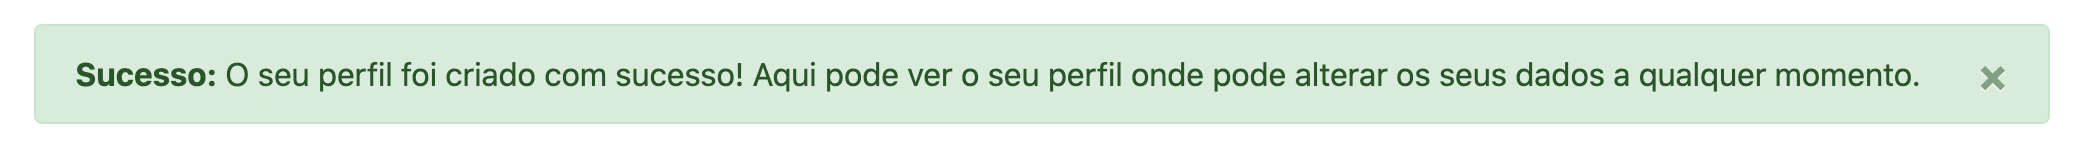
\includegraphics[scale=0.45]{images/alerts/alerta_sucesso.png}
    \caption{Alerta de Sucesso.}
    \label{fig:alertasucesso}
\end{figure}

\subsubsection{Descrição da mensagem de aviso}
\hspace{5mm} O alerta de Aviso é utilizado quando ocorre algum problema, no entanto não impede a continuidade da acção.

\begin{figure}[H]
    \centering
    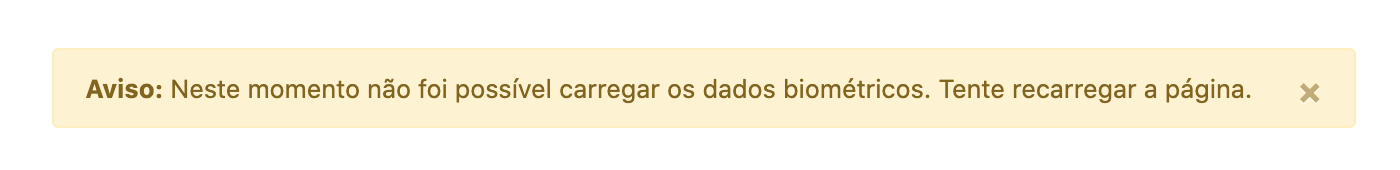
\includegraphics[scale=0.65]{images/alerts/alerta_aviso.png}
    \caption{Alerta de Aviso.}
    \label{fig:alertaaviso}
\end{figure}

\subsubsection{Descrição da mensagem de erro}
\hspace{5mm} O alerta de Erro é utilizado quando o utilizador introduz dados inválidos ou quando existem erros internos dos servidores.

\begin{figure}[H]
    \centering
    
\includegraphics[scale=0.45]{images/alerts/alerta_erro.png}
    \caption{Alerta de Erro.}
    \label{fig:alertaerro}
\end{figure}

\subsubsection{Princípios de usabilidade}
\begin{itemize}
    \item \textbf{Synthesizability}: as mensagens de erro, sucesso ou aviso informam o utilizador do estado do sistema. Desta forma, \textbf{visto que as mensagens ocorrem em todas as páginas, pode-se afirmar que este princípio também}.
    \item \textbf{Generability}: visto que é genérico a todas as views, ou seja, igual em todas as views, mudando apenas o conteúdo da mensagem.
    \item \textbf{Consistency}: tal com foi referido, todas as views implementam as mensagens de erros, sucesso e avisos, logo, torna-se consistente.
\end{itemize}

\subsubsection{Heurísticas de Normam}
\begin{itemize}
    \item \textbf{Visibility of system status}: as mensagens mantém o utilizador informado sobre o que está a acontecer, ou o estado da aplicação.
    \item \textbf{Consistency and standards e Aesthetic and minimalist design}: o design usado para as mensagens de erro são \textbf{minimalista} e \textbf{comum}/\textbf{padrão}, tal como se pode ver nas imagens \ref{fig:alertasucesso}, \ref{fig:alertaaviso} e \ref{fig:alertaerro}.
    \item \textbf{Help users recognize and recover from errors}: as mensagens de erro são bastante informativas na medida do necessário em informar o que aconteceu, bem como dar uma possível solução para o problema ou alternativa.
\end{itemize}

\subsection{Login}
\label{subsec:login}

\subsubsection{Descrição}
\hspace{5mm} De forma a facilitar a autenticação para o utilizador o login é comum aos dois tipos de utilizadores da plataforma, sendo que estes apenas precisam de introduzir as suas credenciais. Podem ainda seleccionar "Registar Cliente" ou "Registar Personal Trainer" caso sejam novos no sistema.

\begin{figure}[H]
    \centering
    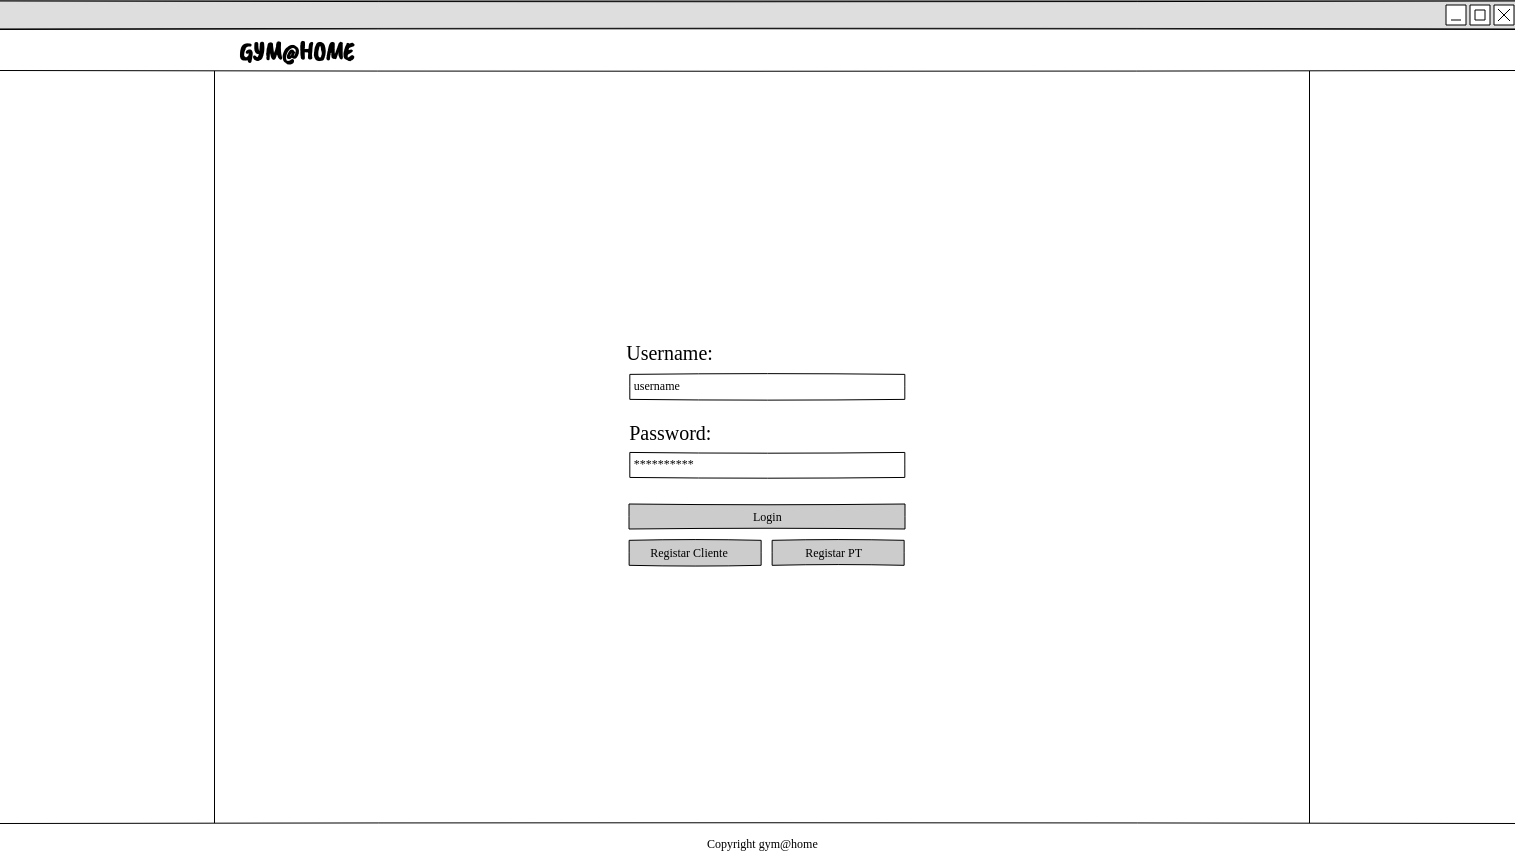
\includegraphics[scale=0.25]{images/mockups/login.png}
    \caption{Mockup Login.}
    \label{fig:mockuplogin}
\end{figure}

\begin{figure}[H]
    \centering
    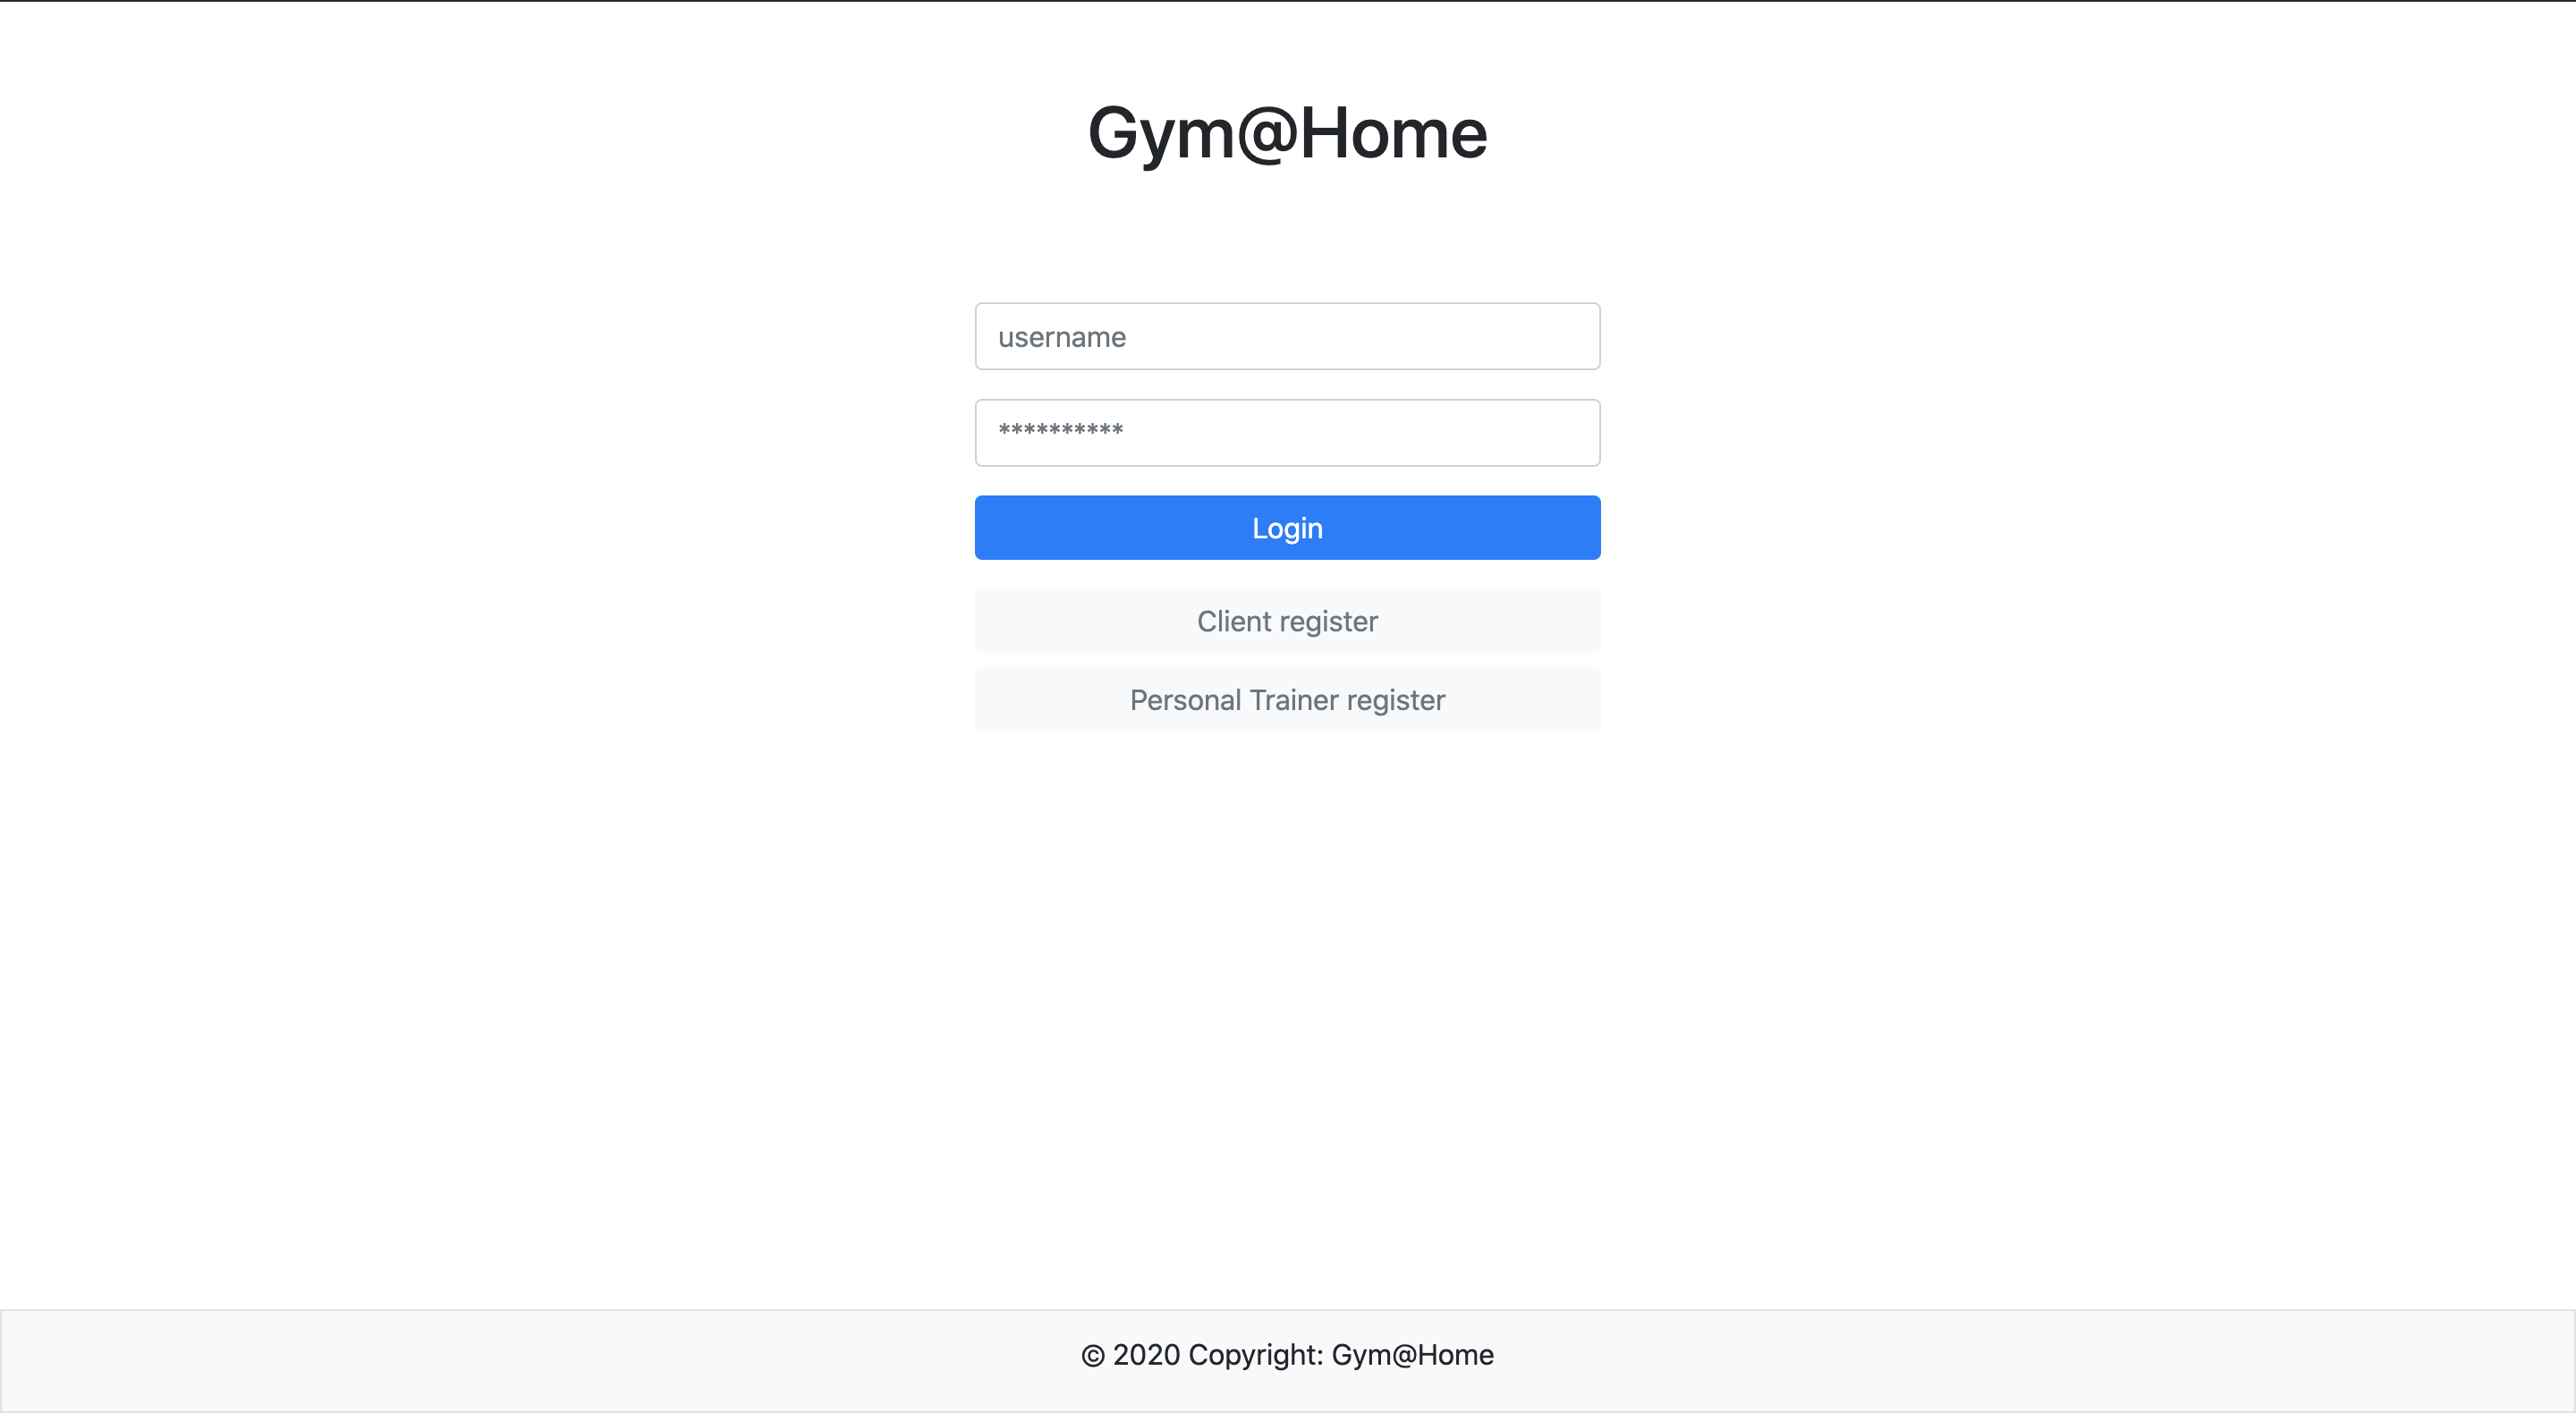
\includegraphics[scale=0.25]{images/interfaces/login.png}
    \caption{Interface Login.}
    \label{fig:interfacelogin}
\end{figure}

\subsubsection{Princípios de usabilidade}
\begin{itemize}
    \item \textbf{Predictability}: o utilizador percebe o efeito das acções, neste caso, fazer o login ou registar-se.
    \item \textbf{Familiarity}: seguiu-se o padrão de desenho de logins presente normalmente em maior parte das aplicações web.
    \item \textbf{Consistency}: bastante semelhante ao anterior, na medida em que o princípio da consistência torna-se mais abrangente.
\end{itemize}

\subsubsection{Heurísticas de Normam}
\begin{itemize}
    \item \textbf{Visibility of system status}: o resultado do login é confirmado com um mensagem de erro ou sucesso dependendo da situação, informando do que está a acontecer.
\end{itemize}

\subsection{Notificações}
\label{subsec:notificacoescliente}

\subsubsection{Descrição}
\hspace{5mm} Com esta mockup tanto o cliente, como o PT consegue saber todas as acções que aconteceram relacionadas com o mesmo. Aqui pode consultar as notificações, isto é, a data, o estado e a descrição bem como marcar como lidas.

\begin{figure}[H]
    \centering
    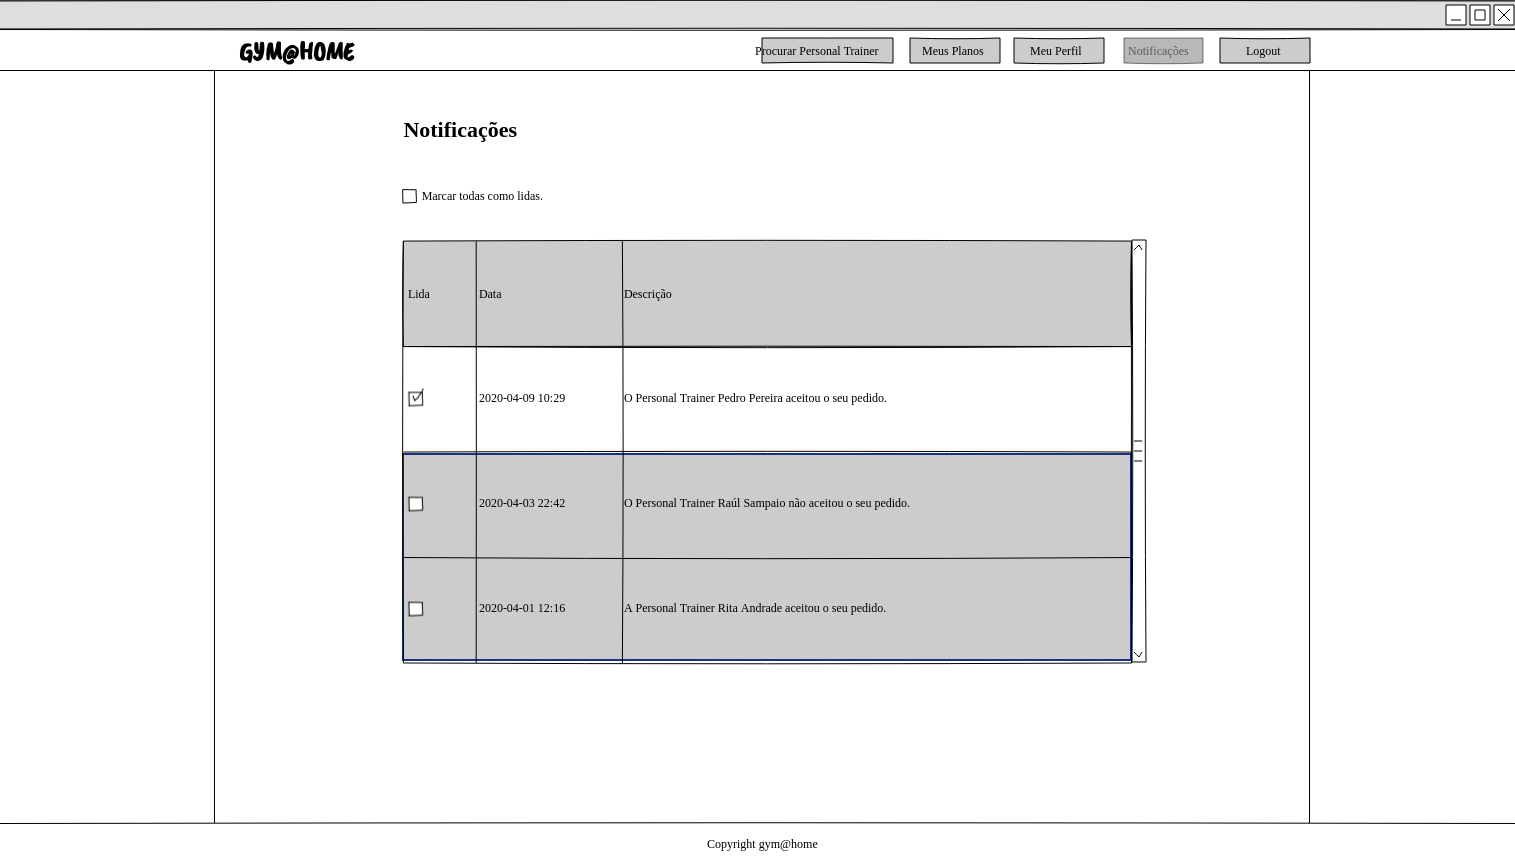
\includegraphics[scale=0.25]{images/mockups/cliente_notificaes.png}
    \caption{Mockup Notificações Cliente.}
    \label{fig:mockupnotificacoescliente}
\end{figure}

\begin{figure}[H]
    \centering
    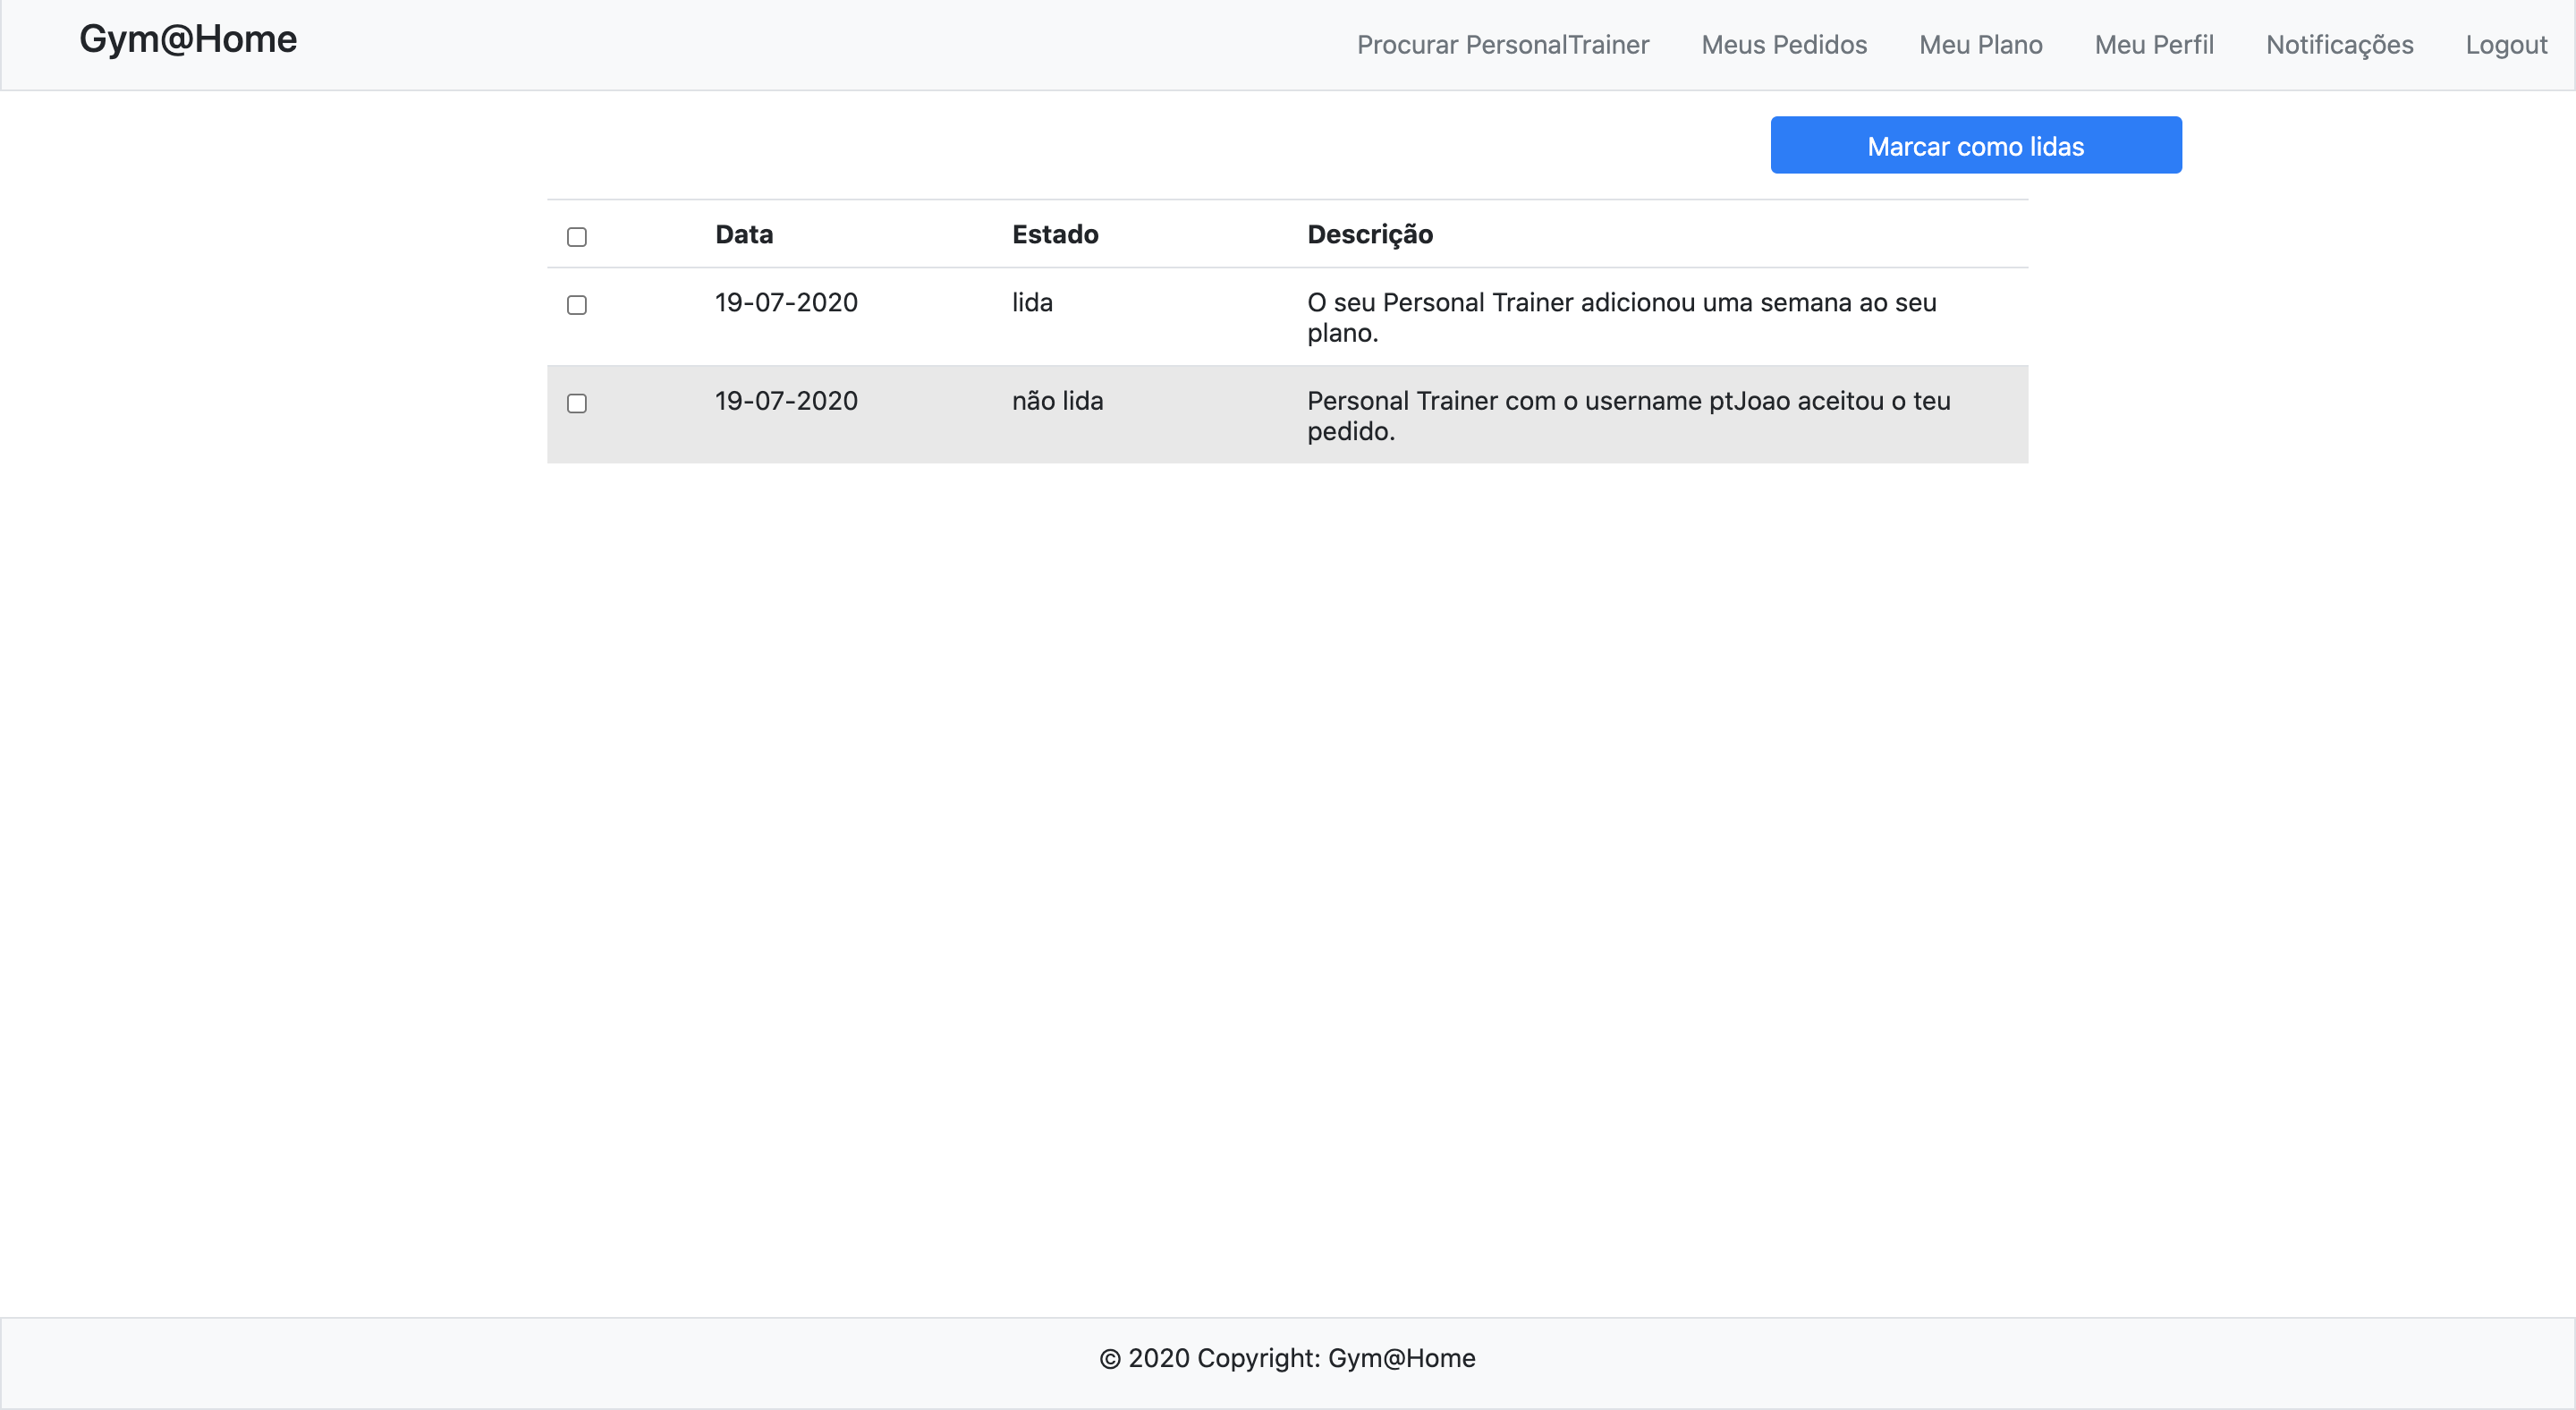
\includegraphics[scale=0.25]{images/interfaces/client_notifications.png}
    \caption{Interface Notificações Cliente.}
    \label{fig:interfacenotificacoescliente}
\end{figure}

\subsubsection{Princípios de usabilidade}
\begin{itemize}
    \item \textbf{Predictability}: quando se selecciona a checkbox para seleccionar todas as notificações para marcar como lidas, apenas selecciona as não lidas, para evitar que se envie o pedido de marcar como lida para o servidor desnecessariamente para notificações que já estão lidas
    \item \textbf{Synthesizability}: após marcar como lidas, as notificações aparecem com uma cor de background diferente, permitindo ao utilizador perceber o efeito da sua acção.
    \item \textbf{Familiarity}: As notificações por ler tem uma cor diferente das notificações lidas, um padrão \textbf{comum}.

\end{itemize}

\subsubsection{Heurísticas de Normam}
\begin{itemize}
    \item \textbf{Visibility of System Status}: os utilizadores obtém informações sobre acções que acontecerem no sistema relacionadas com os mesmos, mas sem ter sido este a alterar o estado.
    \item \textbf{Error Prevetion}: quando selecciona o marcar todas como lidas, apenas selecciona as não lidas, para que não sejam mandados pedidos para o servidor desnecessariamente, tal como já tinha sido dito no princípio de \textbf{Predictability}.
\end{itemize}

%--------------------------------------------------------------------------%

\section{Interfaces Clientes}
\label{sec:mockupsclients}

\subsection{Registar Cliente}
\label{subsec:registarcliente}

\subsubsection{Descrição}

\hspace{5mm} De forma a que o Cliente se registe na aplicação é necessário este inserir alguns dados obrigatórios, tais como o nome, username, email, etc..., bem como dados opcionais relacionados com dados biométricos. No entanto, importante referir que dos dados obrigatórios excepcionalmente a altura e peso são dados obrigatórios.

\begin{figure}[H]
    \centering
    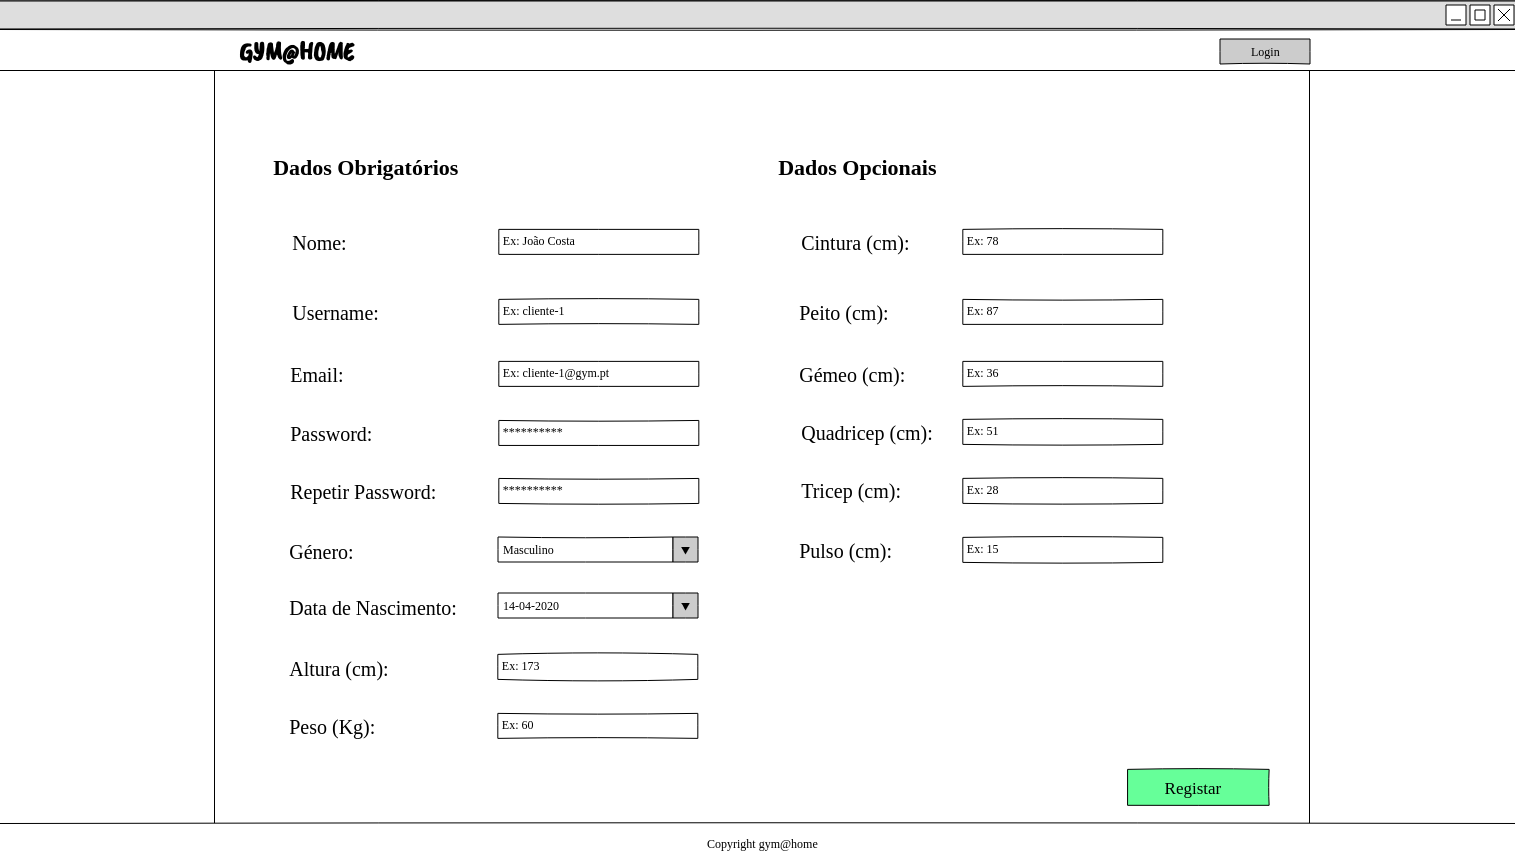
\includegraphics[scale=0.25]{images/mockups/cliente_registo_.png}
    \caption{Mockup Registar Cliente.}
    \label{fig:mockupregistarcliente}
\end{figure}

\begin{figure}[H]
    \centering
    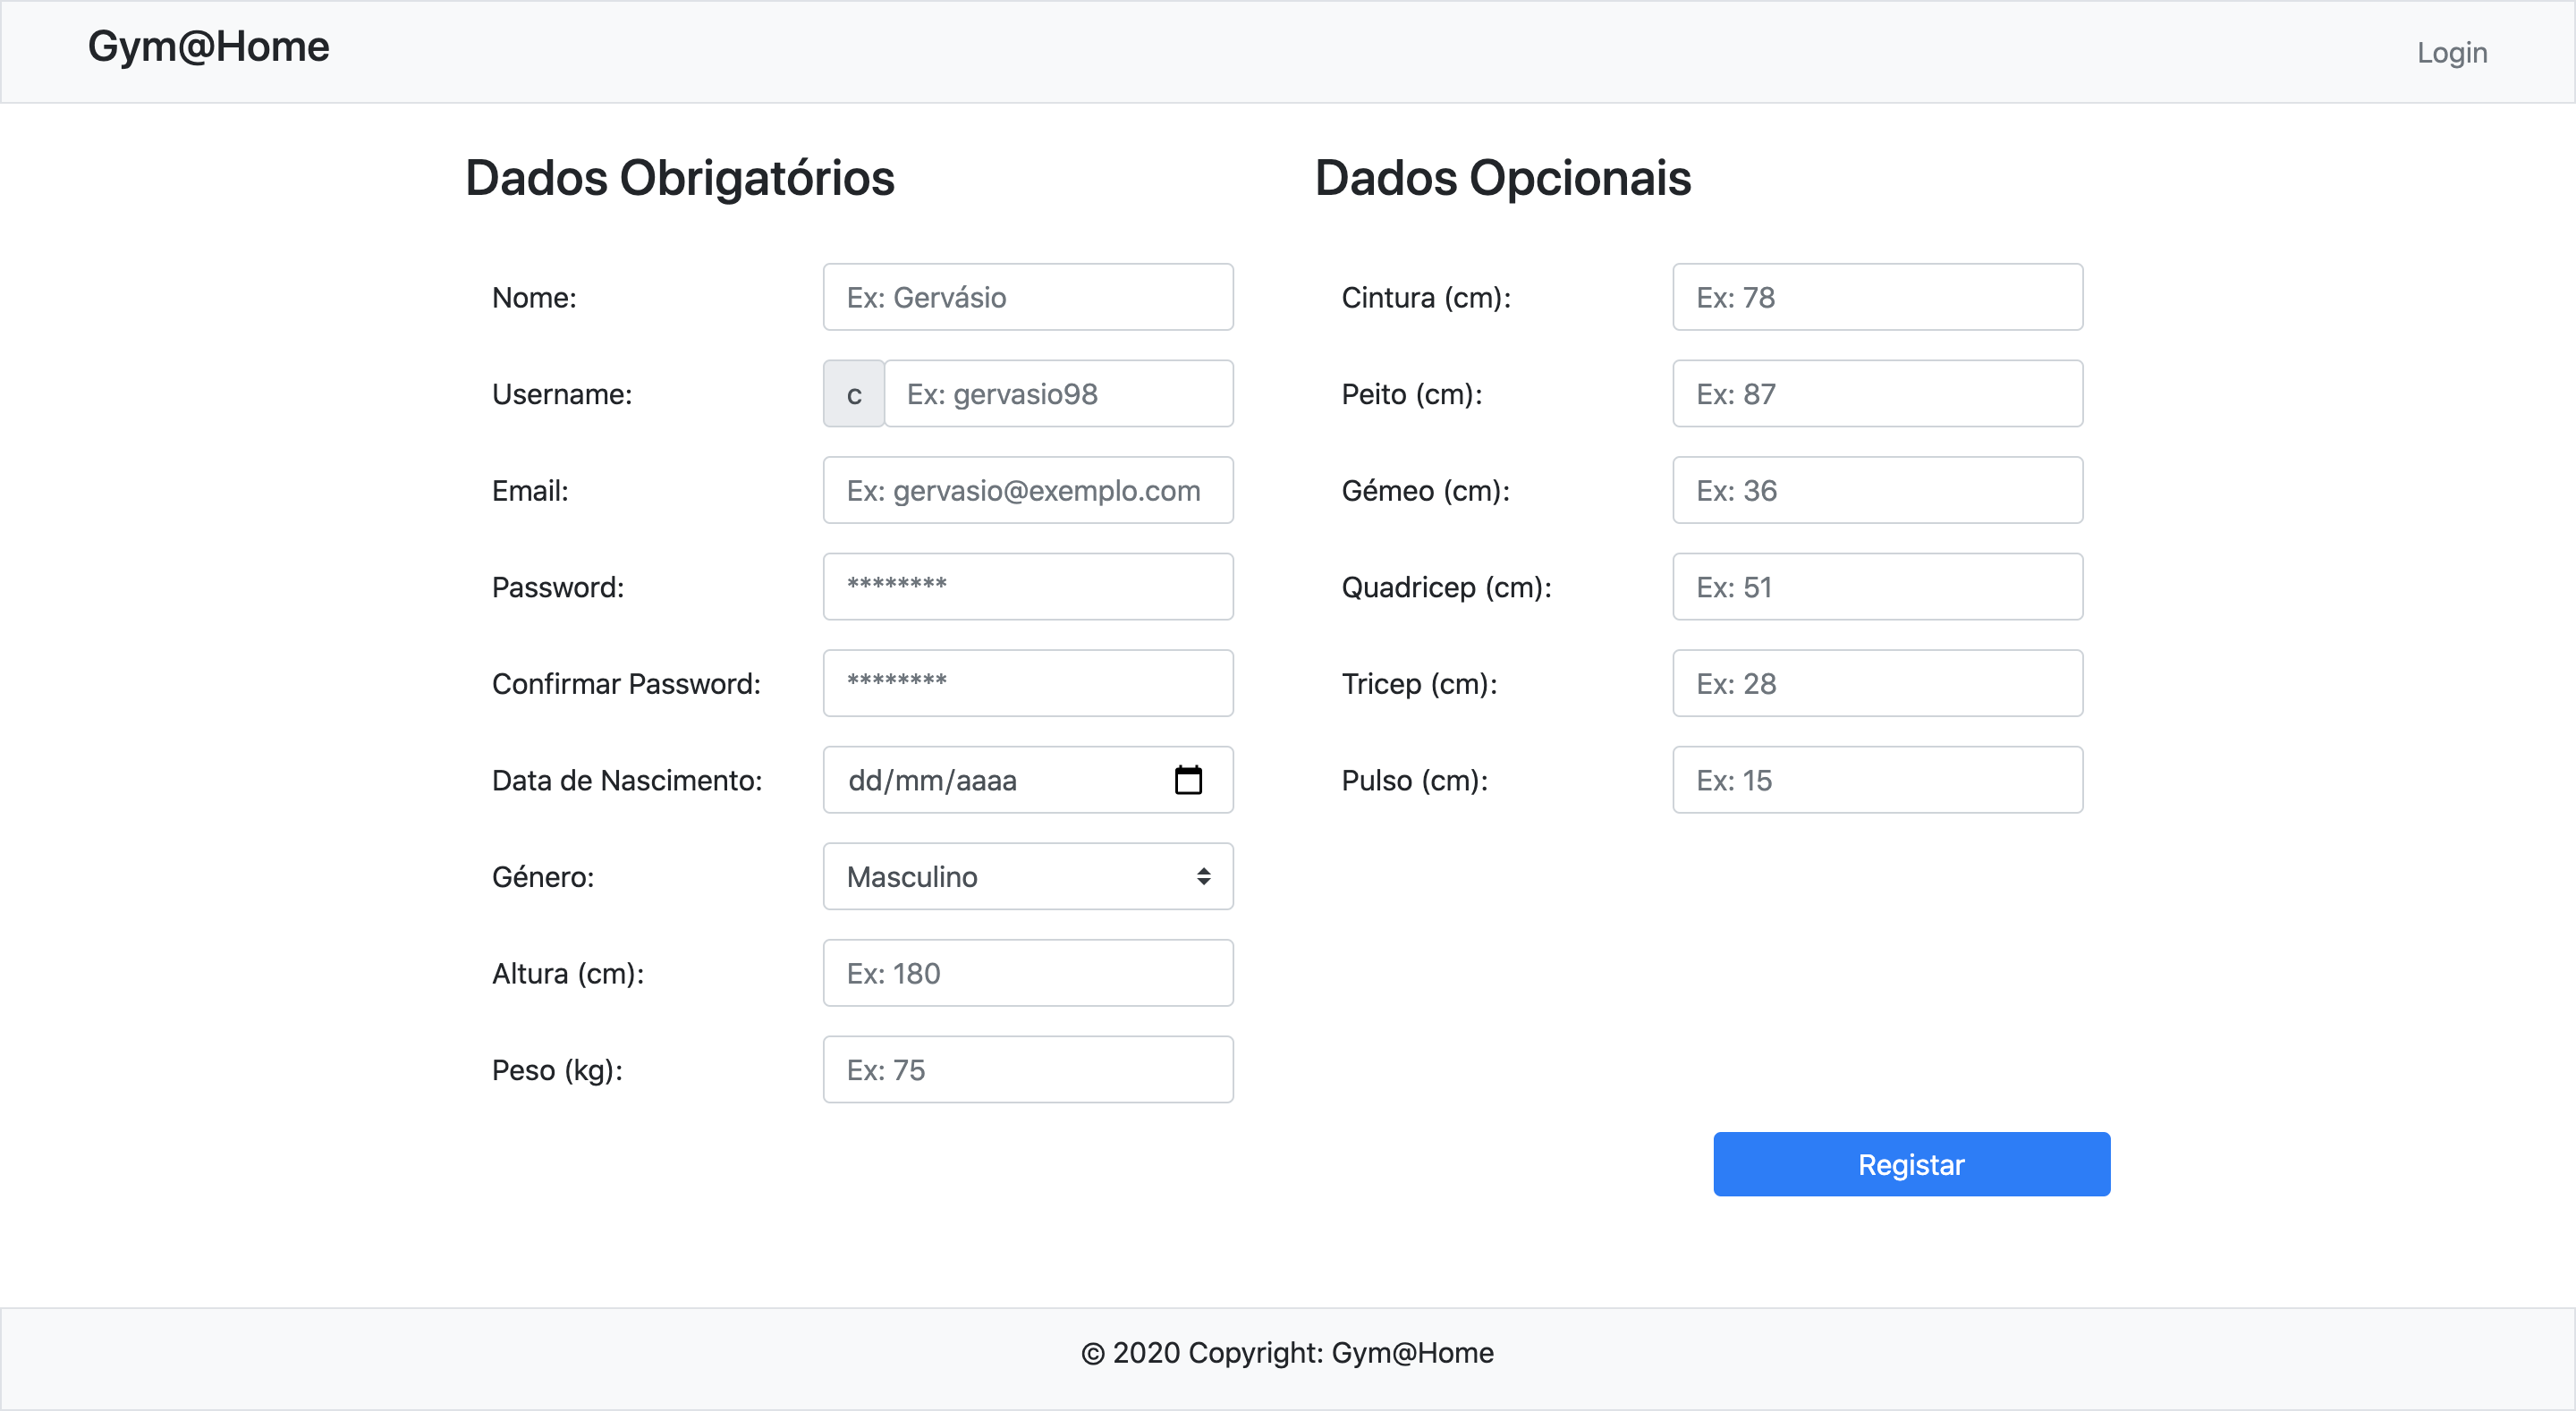
\includegraphics[scale=0.25]{images/interfaces/client_register.png}
    \caption{Interface Registar Cliente.}
    \label{fig:interfaceregistarcliente}
\end{figure}

\subsubsection{Princípios de Usabilidade}
\begin{itemize}
    \item \textbf{Familiarity}: Colocar a "Data de Nascimento" é feito através de um calendário, pelo que o Cliente como ser humano está mais familiarizado a utilizar.
    
\end{itemize}

\subsubsection{Heurísticas de Normam}
\begin{itemize}
    \item \textbf{Error prevention}: Todos os inputs numéricos aceitam apenas números, o "Género" apenas permite os valores do dropdown, a "Data de Nascimento" apenas permite datas seleccionadas pelo calendário e o "Email" apenas aceita um email (tem de conter o @).
    \textbf{Flexibility and efficiency of use}: visto que após ser feito o registo, faz-se o login automático, sendo mais \textbf{eficiente para o cliente}.
    
\end{itemize}

\subsection{Cliente consulta/edita o próprio perfil}
\label{subsec:perfilclientebycliente}

\subsubsection{Descrição}
\hspace{5mm} O mockup \textsc{Perfil do Cliente}, permite ao Cliente visualizar, bem como, editar o seu próprio perfil para manter as suas informações mais actualizadas possíveis. De forma a ficar mais consistente com o Registo de um Cliente na interface foram mantidas as duas colunas de dados, sendo que no cimo da página ficam os dados pessoais, de seguida os dados biométricos e a barra sobre o estado do IMC segundo os valores de referência da OMS.

\hspace{5mm} A submissão das alterações efectuadas ao perfil, basta alterar os dados que ele necessitar e carregar no botão "Salvar Alterações", este botão de forma a ficar mais visível na interface final foi colocado no cimo da página em vez de estar no fundo da mesma, pois em dispositivos mais pequenos o botão poderia ficar escondido.

\begin{figure}[H]
    \centering
    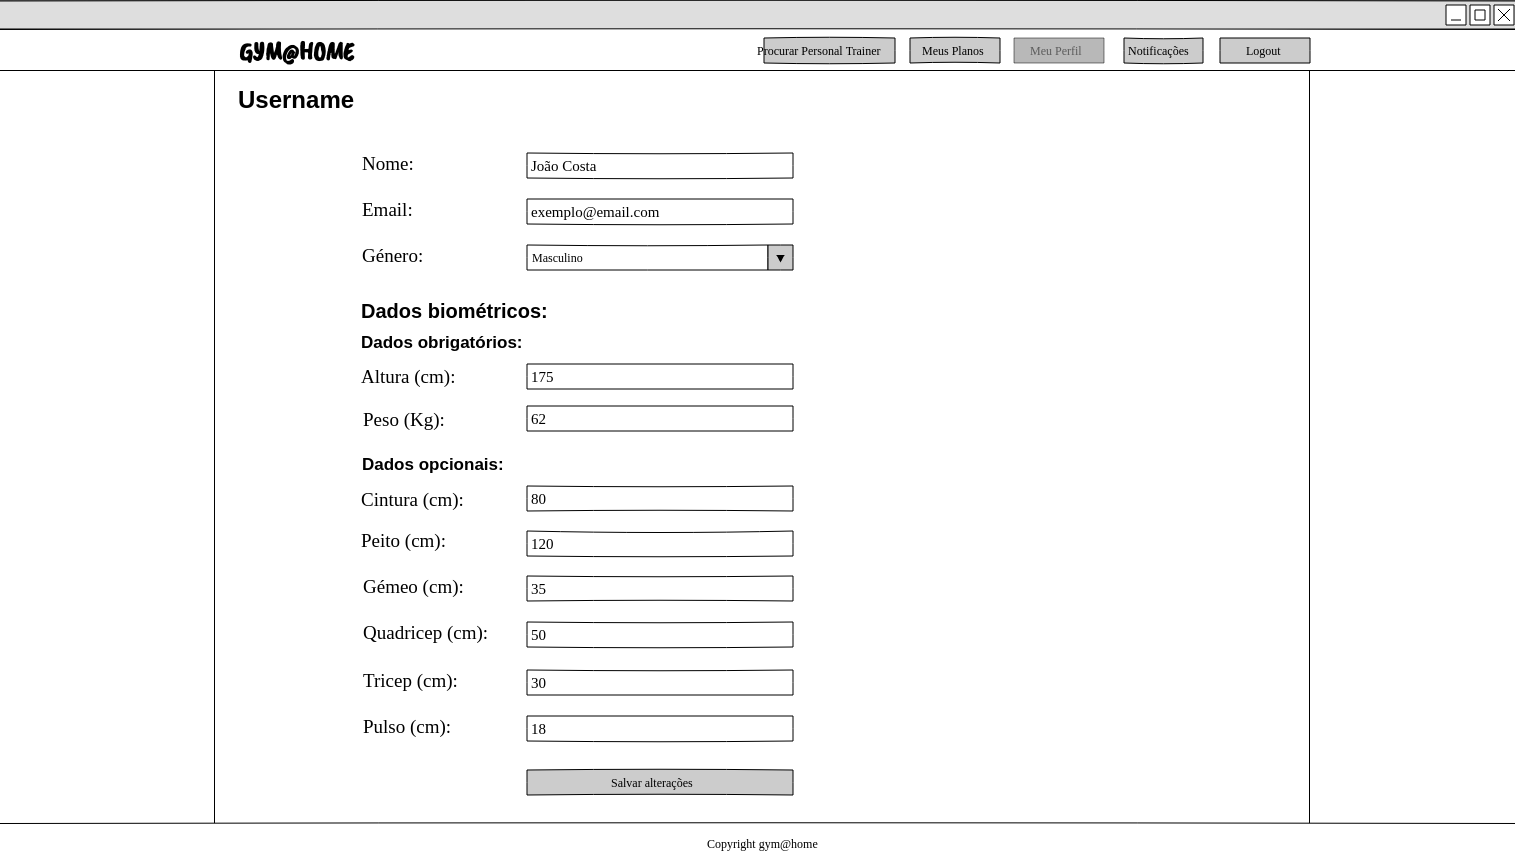
\includegraphics[scale=0.25]{images/mockups/pgina_meu_perfil_cliente.png}
    \caption{Mockup Perfil Cliente visto pelo próprio.}
    \label{fig:mockupperfilclientebycliente}
\end{figure}

\begin{figure}[H]
    \centering
    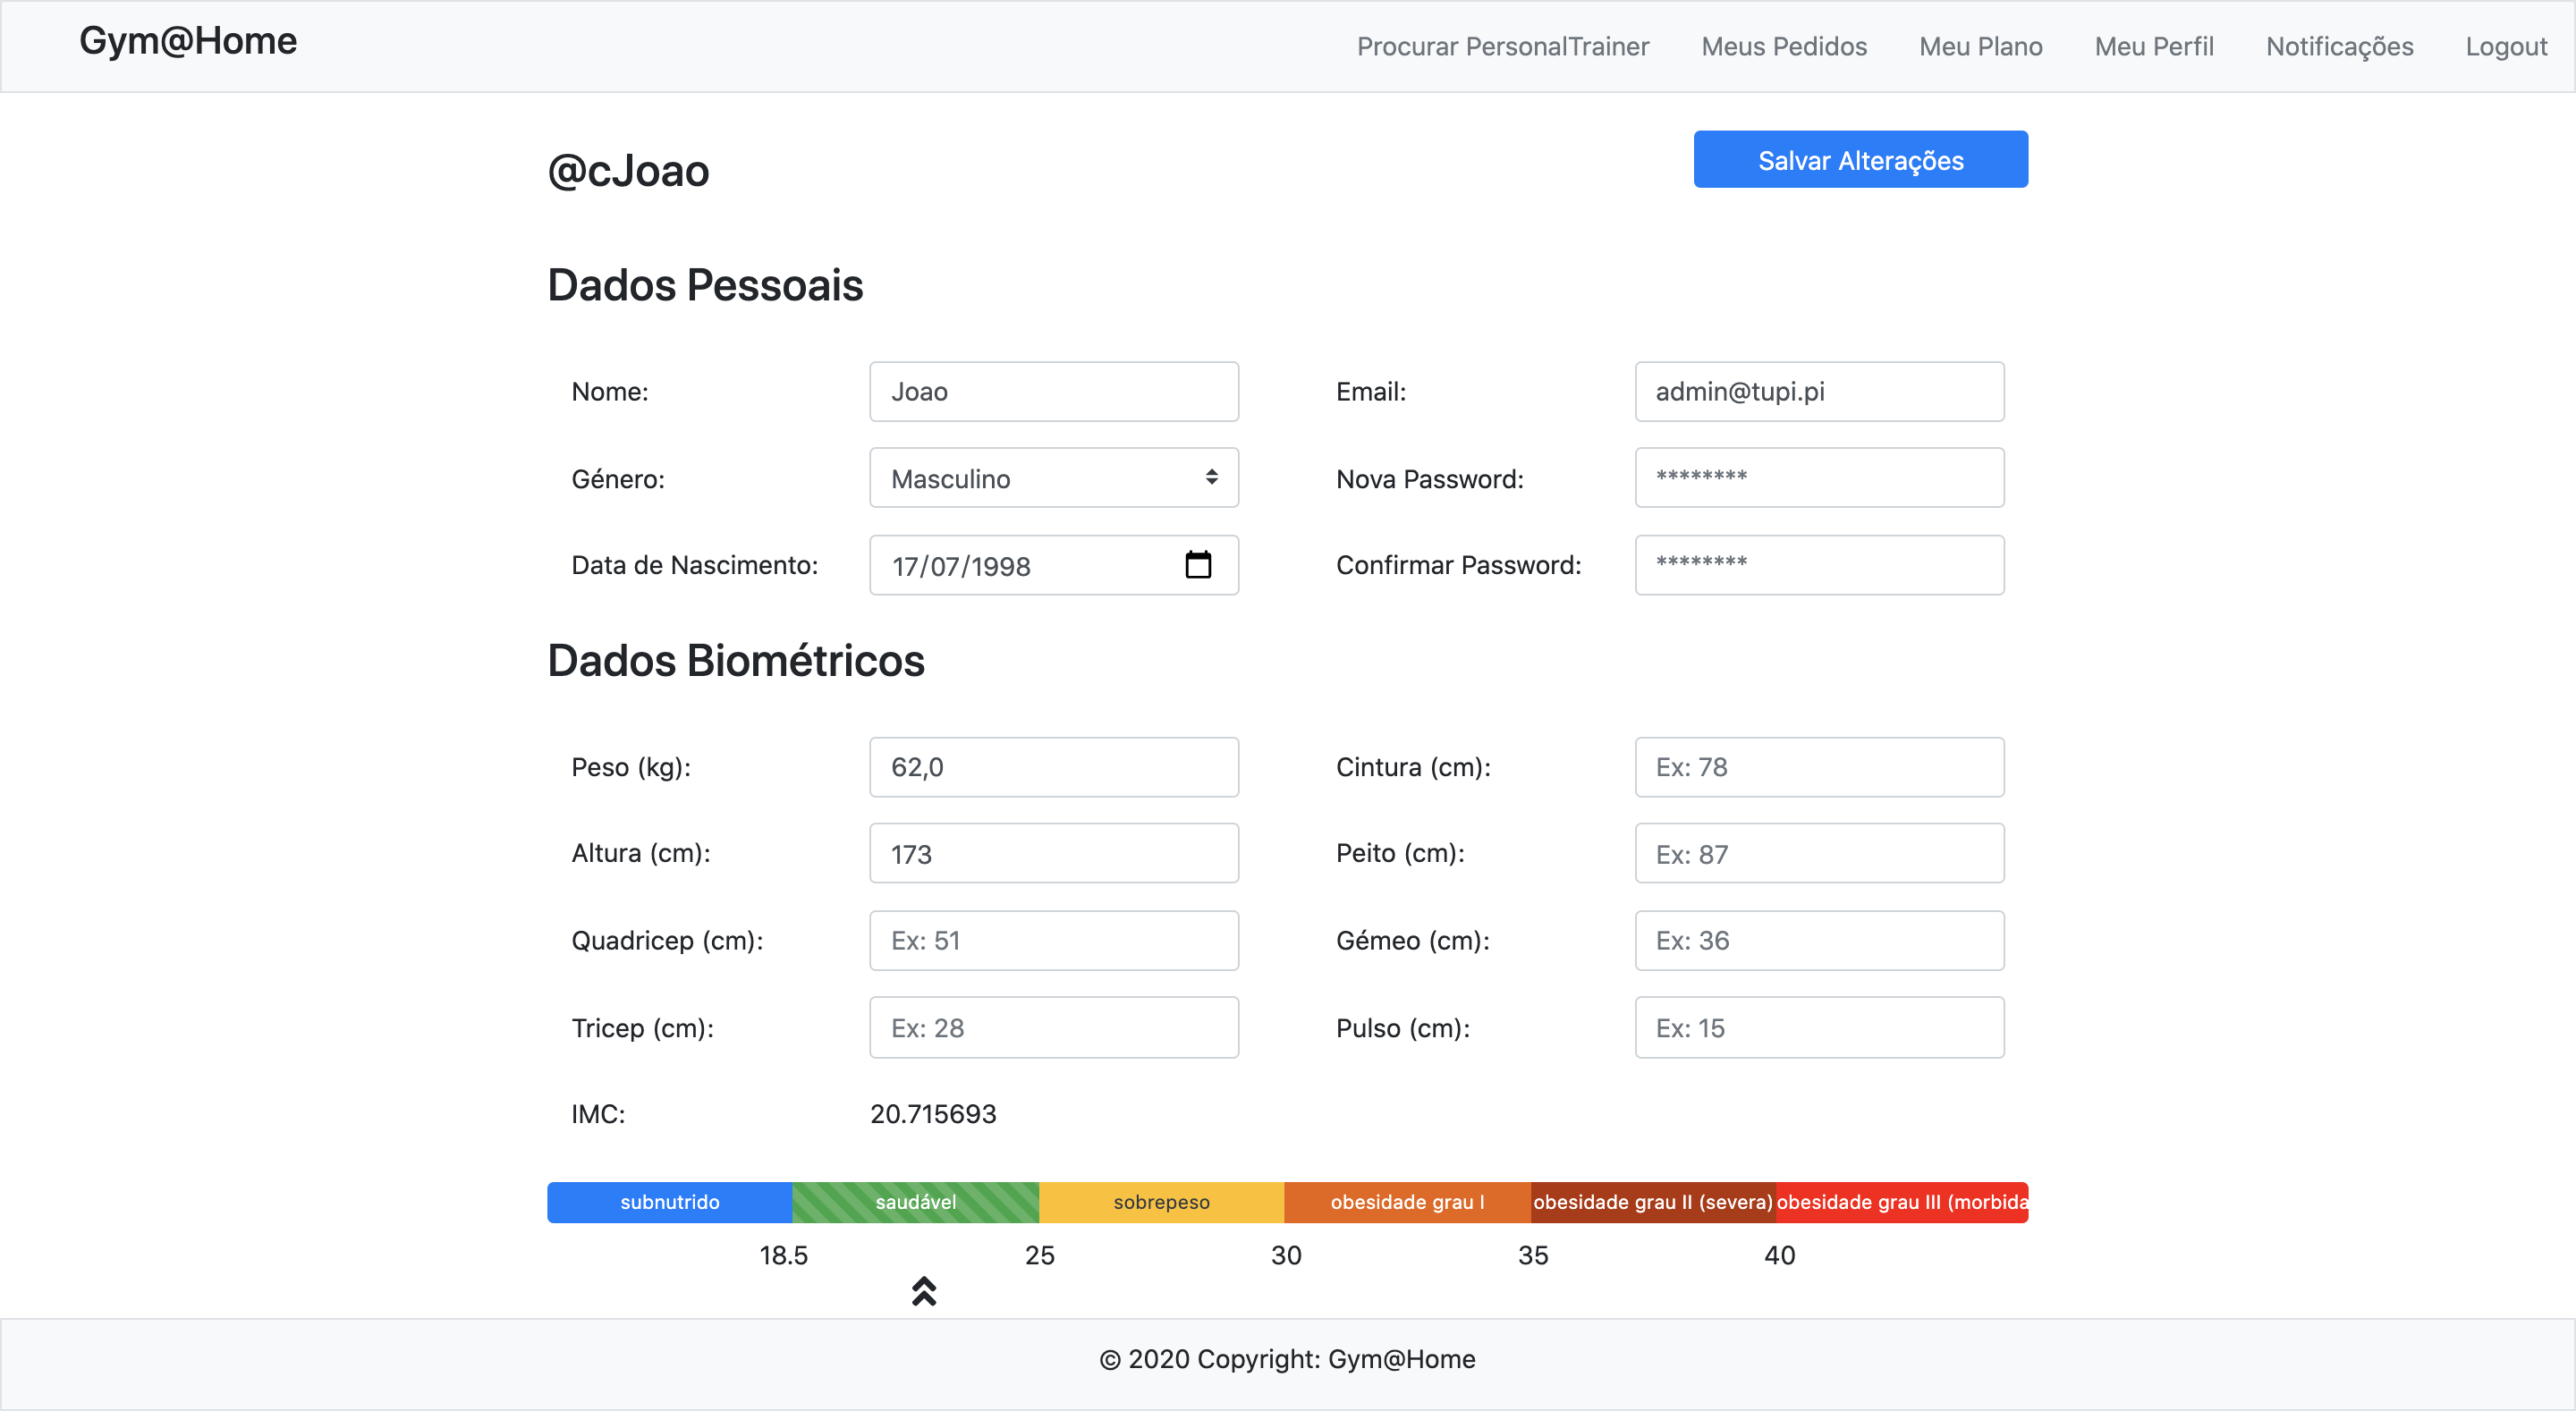
\includegraphics[scale=0.25]{images/interfaces/client_perfil.png}
    \caption{Interface Perfil Cliente visto pelo próprio.}
    \label{fig:interfaceperfilclientebycliente}
\end{figure}

\subsubsection{Princípios de usabilidade}
\begin{itemize}
   \item \textbf{Substitutivity}: Os inputs da interface onde o Cliente pode alterar os valores são também outputs. Sempre que o Cliente alterar dados estes são guardados na BD e novamente carregados para os outputs que o Cliente tinha utilizado como input.
    
    \item \textbf{Observability}: O botão "Salvar Alterações" está no cimo da página para o Cliente o conseguir observar mal carregue a página.
    
    \item \textbf{Familiarity}: Colocar a "Data de Nascimento" é feito através de um calendário, pelo que o Cliente como ser humano está mais familiarizado a utilizar.
    
\end{itemize}

\subsubsection{Heurísticas de Normam}
\begin{itemize}
    \item \textbf{Error prevention}: Todos os inputs numéricos aceitam apenas números, o "Género" apenas permite os valores do dropdown, a "Data de Nascimento" apenas permite datas seleccionadas pelo calendário e o "Email" apenas aceita um email (tem de conter o @).
    \item \textbf{Flexibility and efficiency of use}: tal como diz respeito ao principio \textbf{Substitutivity}, usar o mesmo componente quer para visualizar, quer para editar o perfil, torna a interface mais eficiente para o PT.
\end{itemize}

\subsection{Cliente consultar o perfil do PT}
\label{subsec:perfilptbycliente}

\subsubsection{Descrição}
\hspace{5mm} De forma a que o Cliente tenha uma visão mais detalhada do PT antes de realizar um pedido de Plano são mostradas algumas estatísticas do mesmo. De forma a que o Cliente disponha da informação do PT sem mudar de página este é ilustrado num pop-up, desta forma os filtros aplicados no refinamento dos PTs a observar são mantidos porque não é feito reload à página de "Procurar Personal Trainer".

\begin{figure}[H]
    \centering
    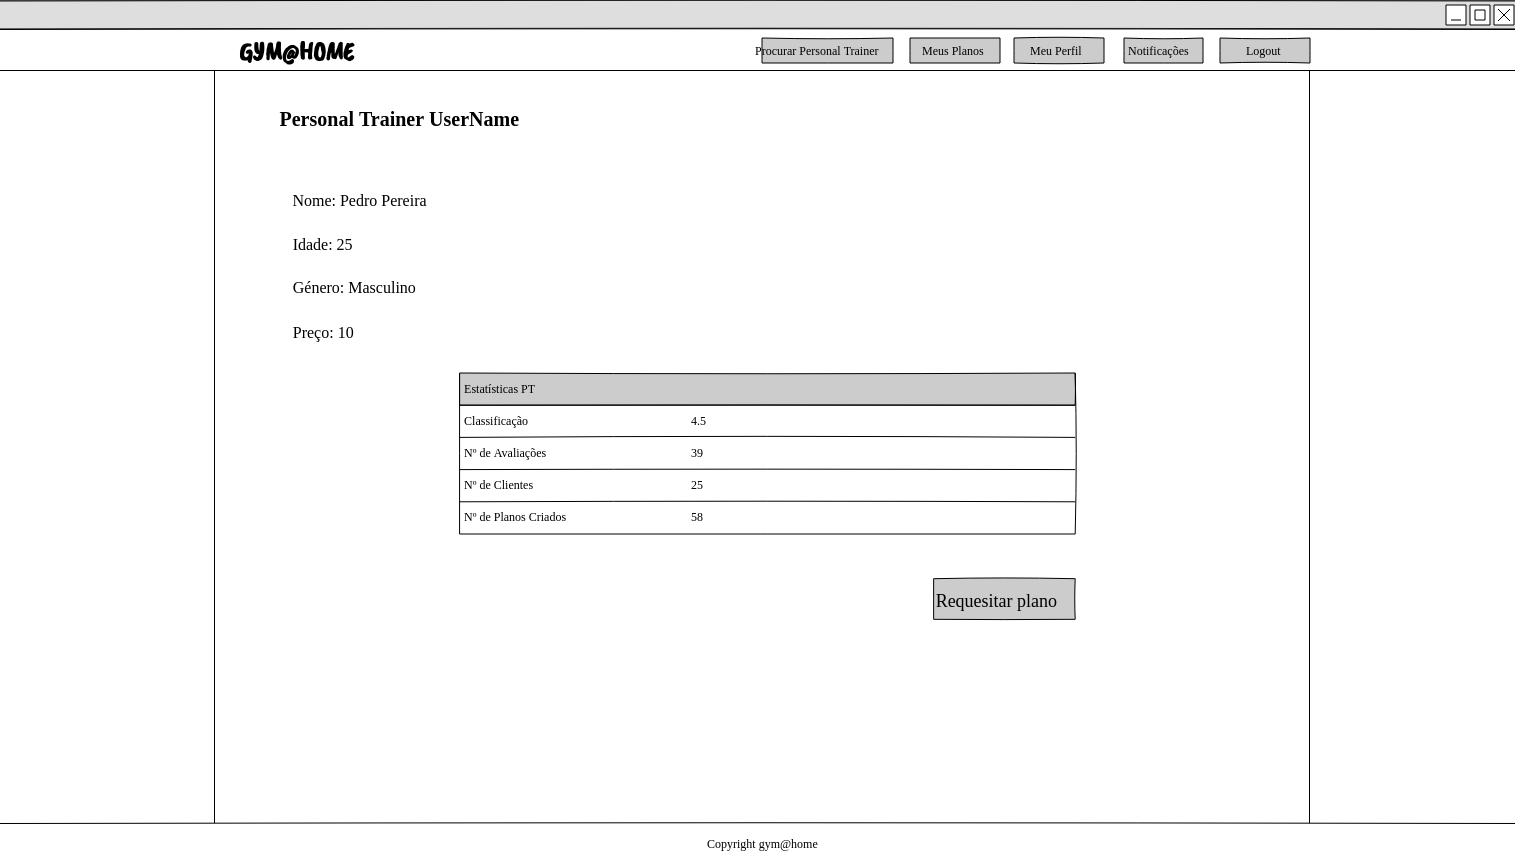
\includegraphics[scale=0.25]{images/mockups/cliente_perfil_personal_trainer.png}
    \caption{Mockup Perfil PT visto pelo Cliente.}
    \label{fig:mockupperfilptbycliente}
\end{figure}

\begin{figure}[H]
    \centering
    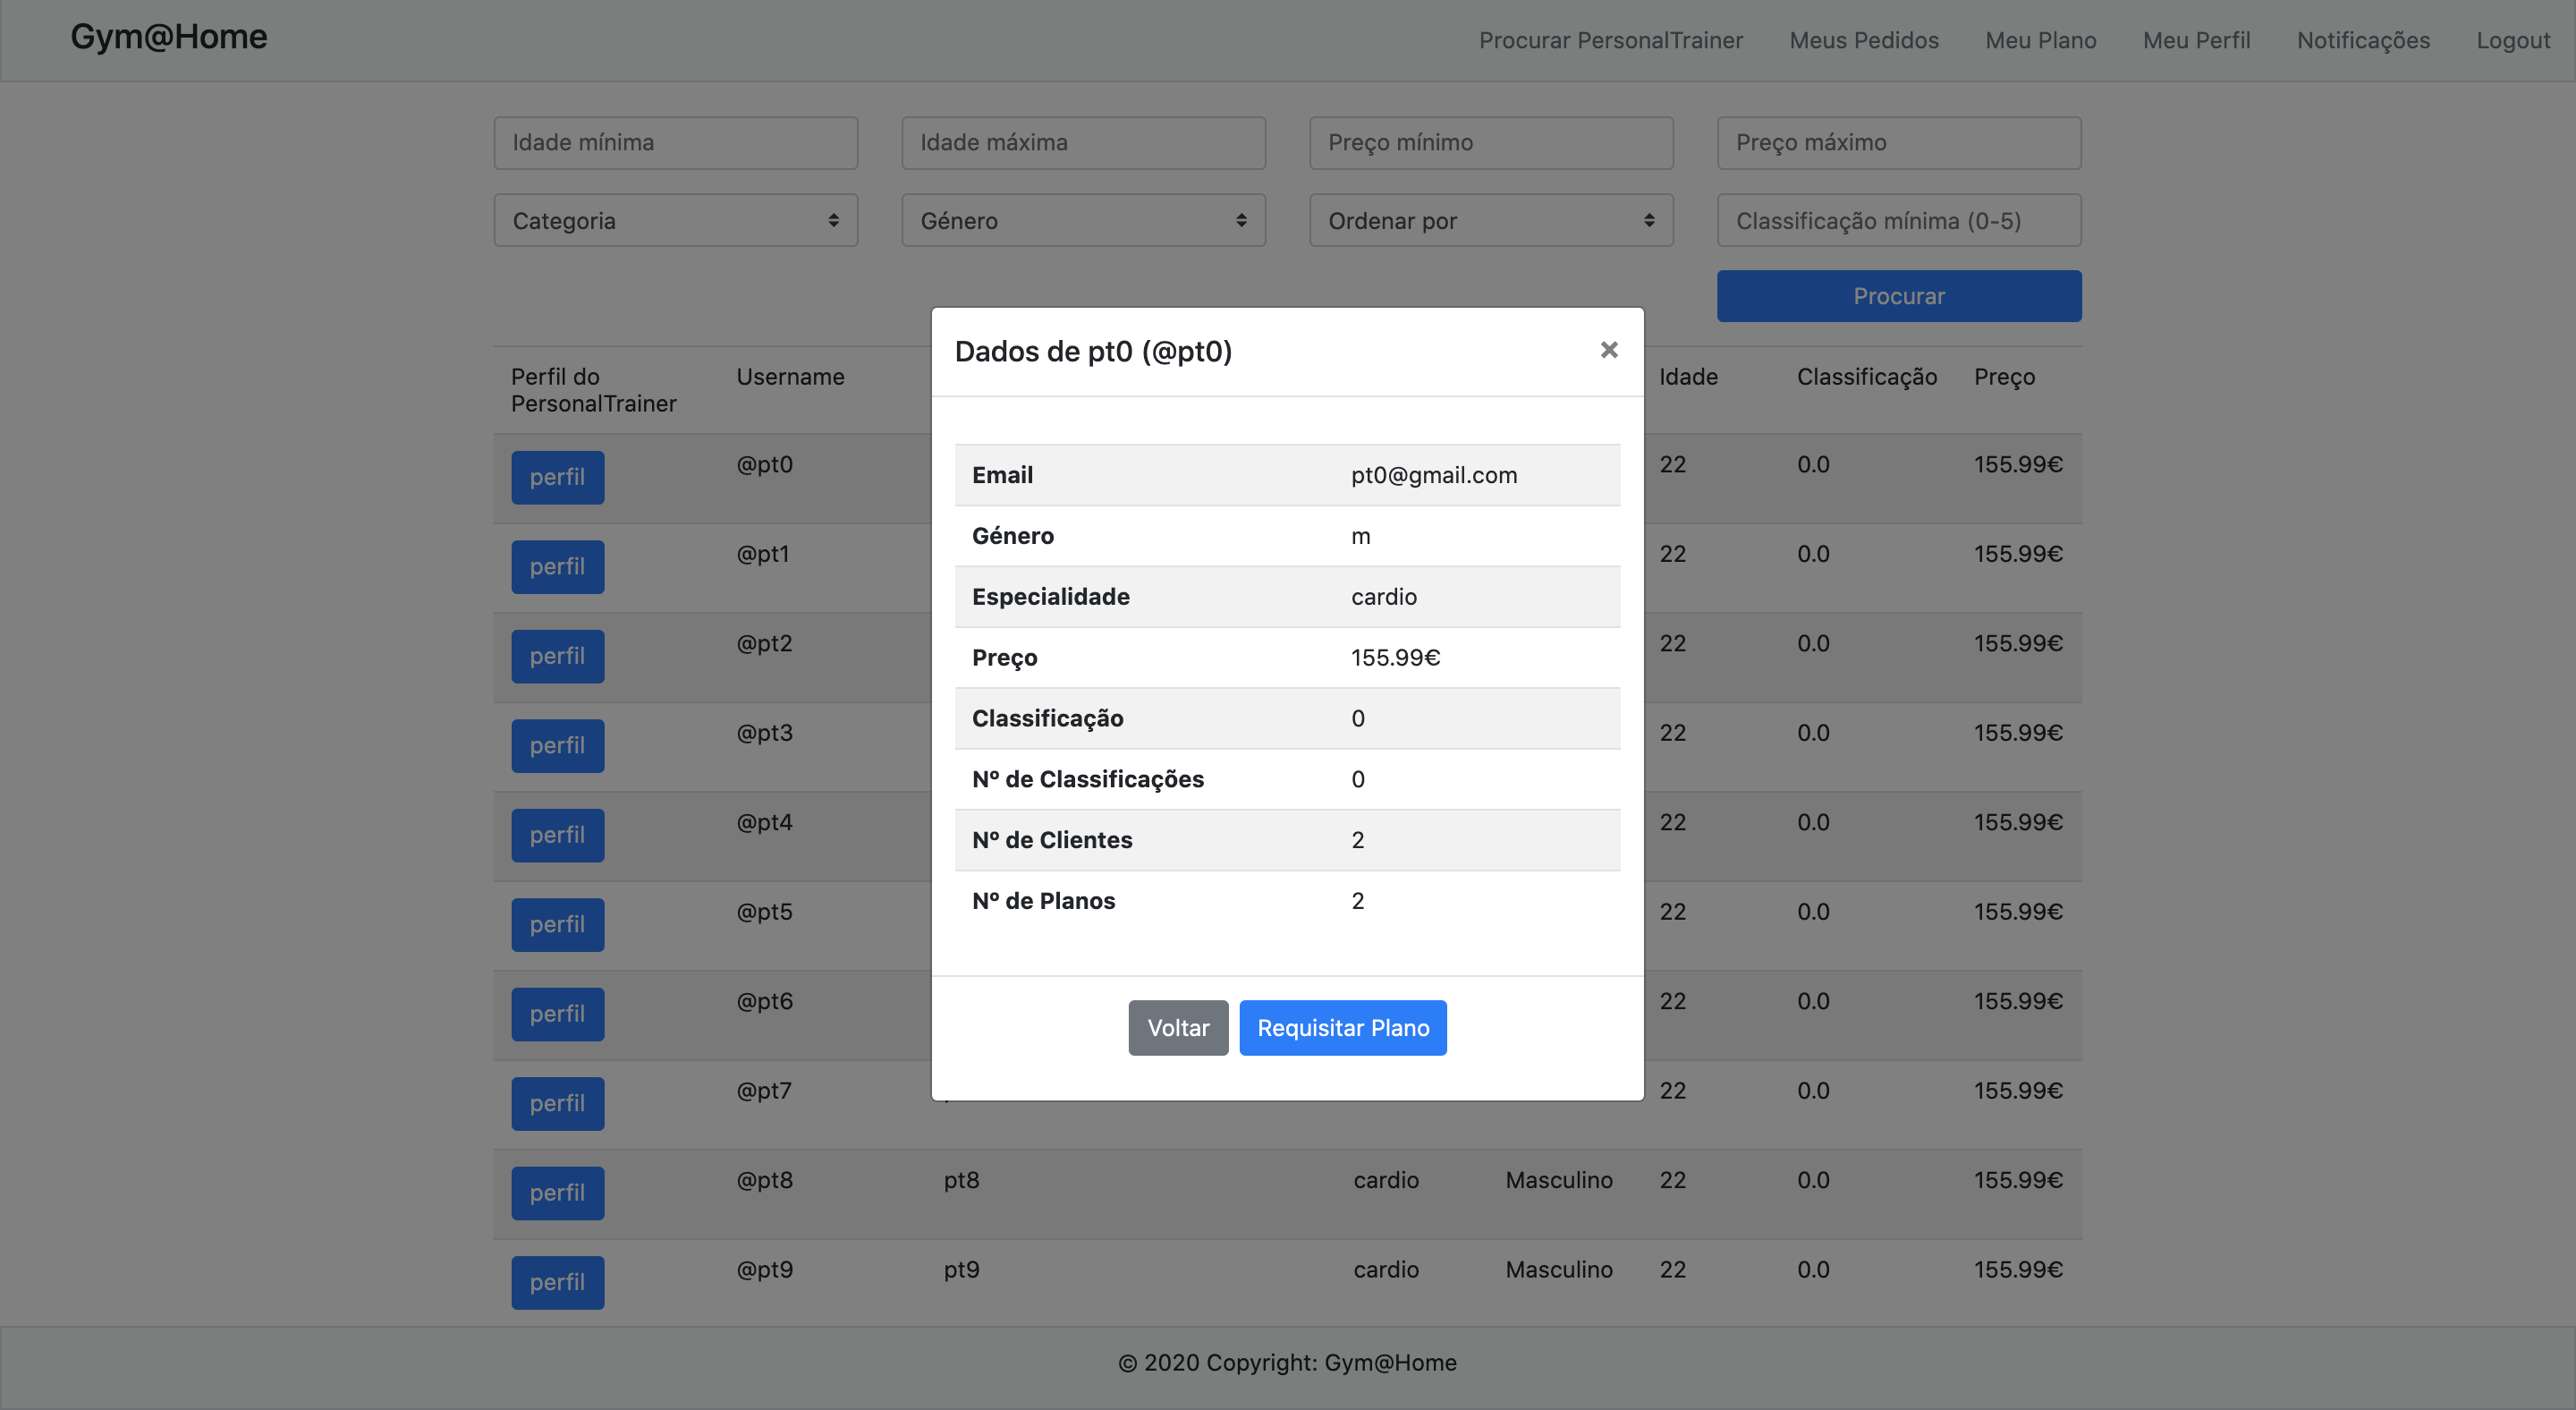
\includegraphics[scale=0.25]{images/interfaces/client_perfil_pt.png}
    \caption{Interface Perfil PT visto pelo Cliente.}
    \label{fig:interfaceperfilptbycliente}
\end{figure}

\subsubsection{Princípios de usabilidade}
\begin{itemize}
    \item \textbf{Generability} e \textbf{Consistency}: na medida em que a estrutura de apresentação deste pop-up com a informação do perfil torna-se semelhante para ambos os utilizadores quando desejam consultar a informação da entidade oposta.
\end{itemize}

\subsubsection{Heurísticas de Normam}
\begin{itemize}
    \item \textbf{Recognition rather than recall}: o cliente não necessita de lembrar-se/memorizar dos dados de perfil do PT, podendo consultá-los no momento em que precisa dos mesmos de forma eficiente.
    \item \textbf{Flexibility and efficiency of use}: o botão "perfil", que mostra as informações do PT torna esse processo de consulta mais \textbf{eficiente}, como uma espécie de atalho.
\end{itemize}

\subsection{Procurar Personal Trainer}
\label{subsec:procurarpersonaltrainer}

\subsubsection{Descrição}
\hspace{5mm} Nesta mockup são ilustrados todos os PTs disponíveis, aqui o Cliente pode aplicar filtros para uma pesquisa mais refinada por PTs que possam ser do seu interesse. Devido ao tamanho dos filtros e respectivo conteúdo estes não cabiam numa única linha tal como na mockup pelo que na interface final estes aparecem em duas linhas, ficando assim mais legíveis para o Cliente.

\hspace{5mm} Tal como foi mostrado no mockup anterior, cada linha, que corresponde a um PT contém um botão denominado "perfil" que apresenta um pop-up com as informações do perfil do PT, onde se encontram algumas informações adicionais.

\begin{figure}[H]
    \centering
    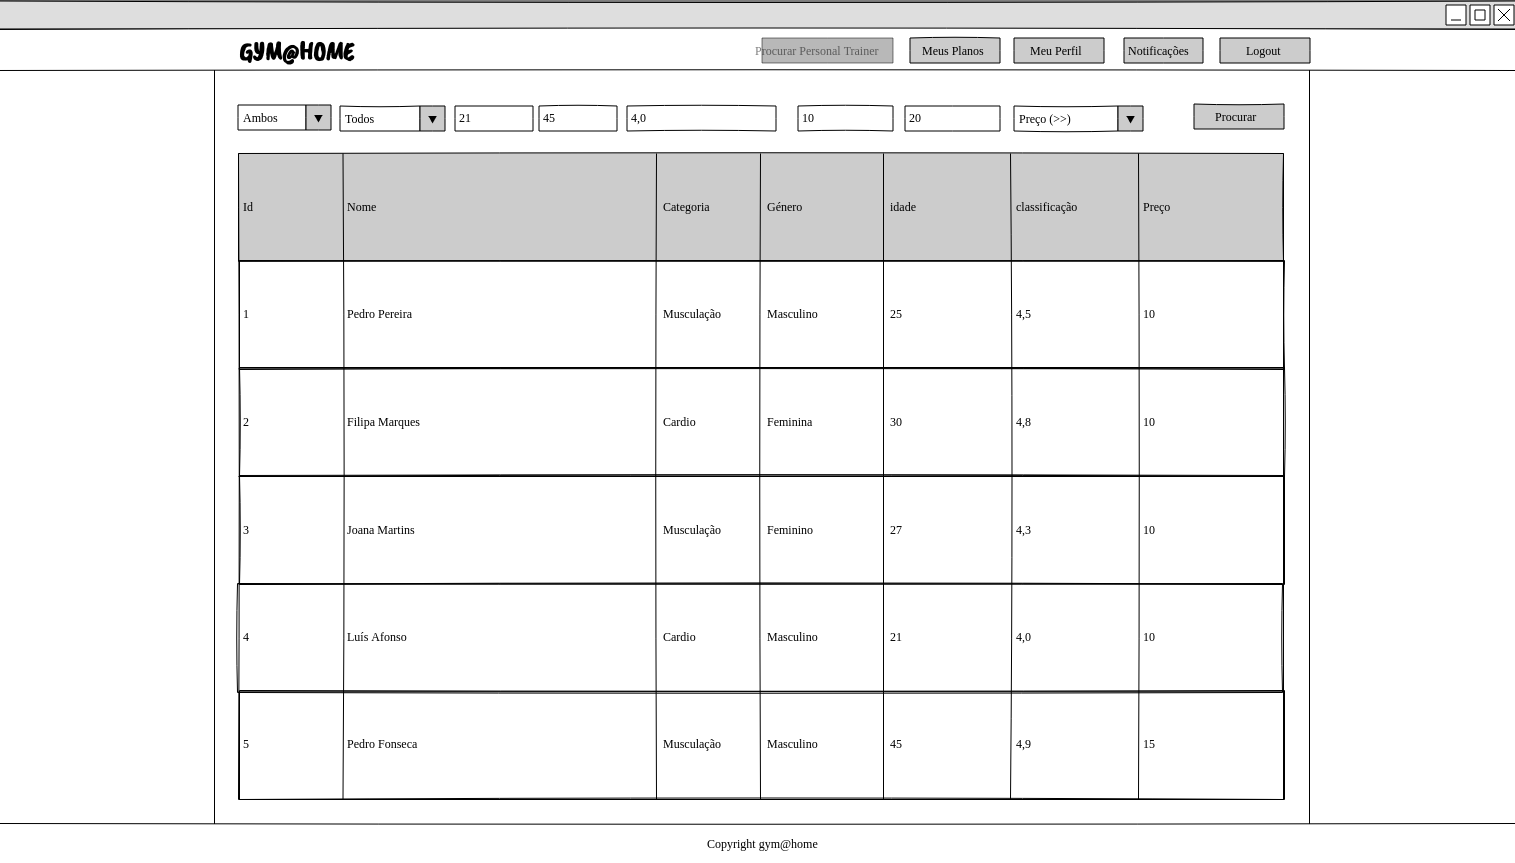
\includegraphics[scale=0.25]{images/mockups/procurar_com_filtros_tabela_preenchida.png}
    \caption{Mockup Procurar Personal Trainer.}
    \label{fig:mockupprocurarpersonaltrainer}
\end{figure}

\begin{figure}[H]
    \centering
    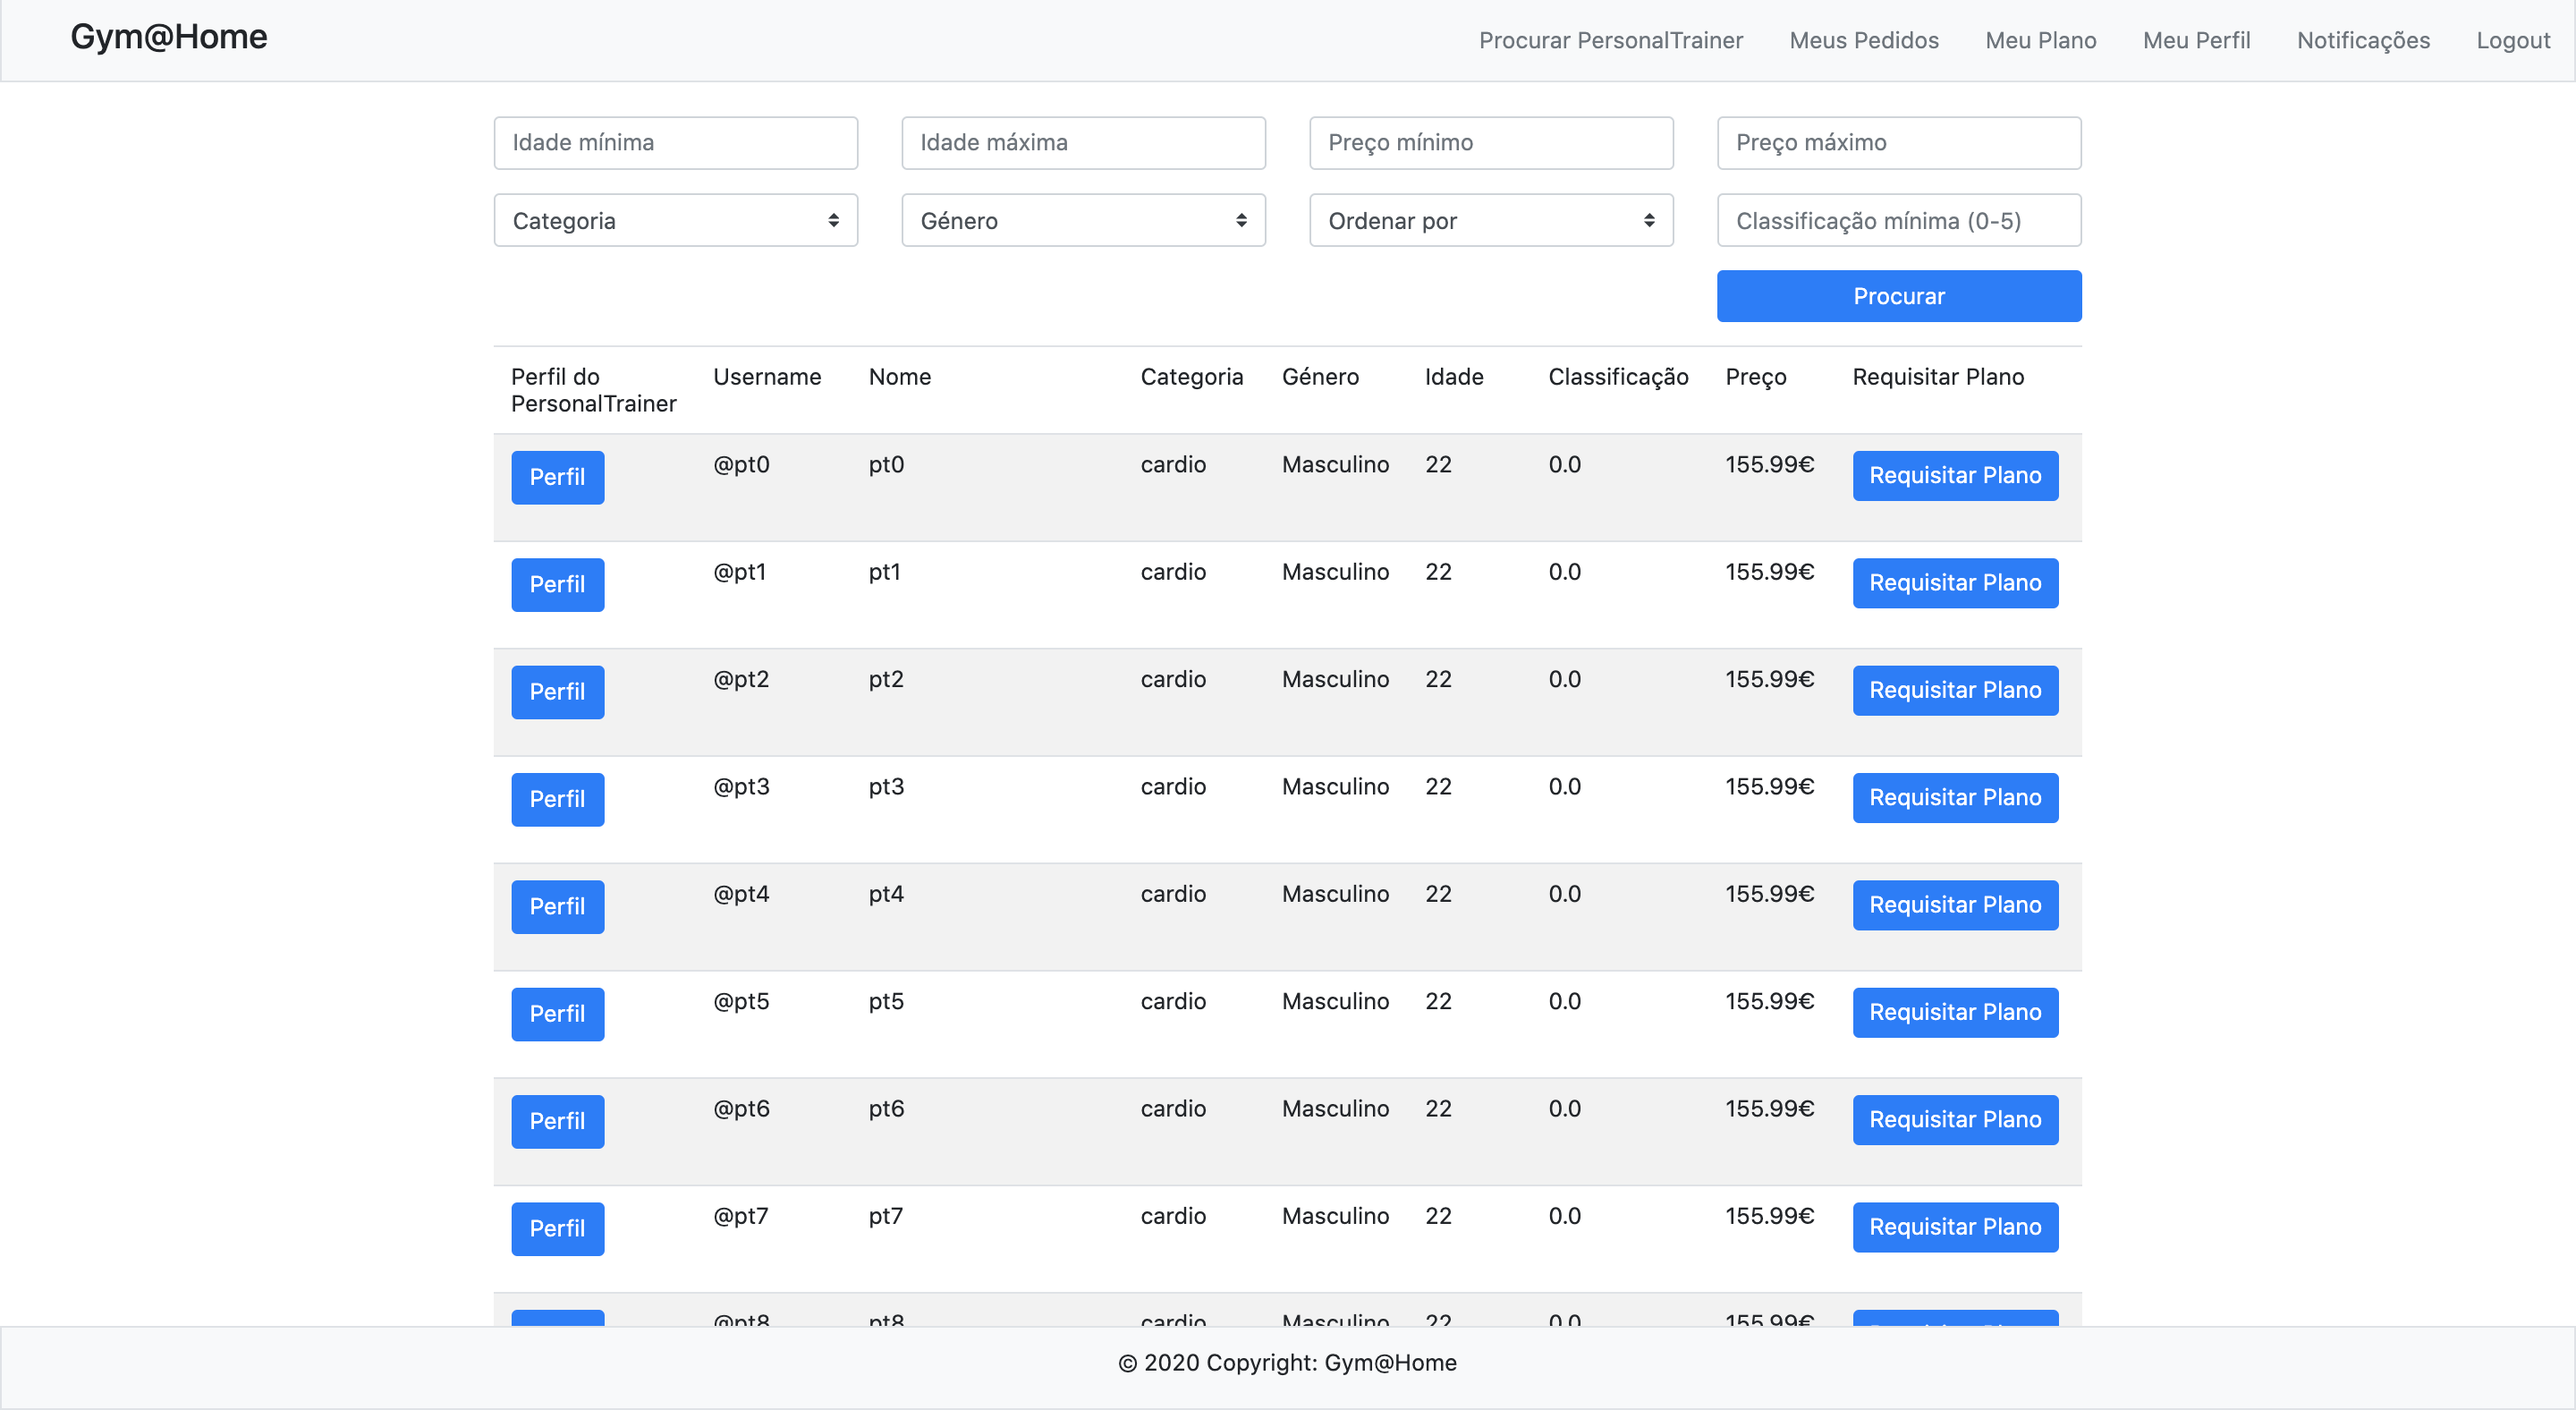
\includegraphics[scale=0.25]{images/interfaces/client_procurar_pt.png}
    \caption{Interface Procurar Personal Trainer.}
    \label{fig:interfaceprocurarpersonaltrainer}
\end{figure}

\subsubsection{Princípios de usabilidade}
\begin{itemize}
    \item \textbf{Synthesizability}: nesta interface, existem duas situações deste princípio: inicialmente quando são listados todos os PTs, isto é, consegue perceber o efeito da sua acção, por outro lado, quando selecciona um PT e deseja requisitar um plano do mesmo, redirecciona-se para a página para esse efeito, e dessa forma, também consegue perceber o efeito da sua acção.
    \item \textbf{Familiarity}: a estrutura utilizada para a filtragem seguiu o padrão comum, que se pode encontrar em muitas aplicações web.
\end{itemize}

\subsubsection{Heurísticas de Normam}
\begin{itemize}
    \item \textbf{Error prevention}: Todos os inputs numéricos aceitam apenas números e o "Género", "Categoria" e "Ordenar Por" apenas permite os valores dos dropdowns.
    \item \textbf{Recognition rather than recall}: utilização de dropdowns nos filtros permite que o utilizador não tenha que memorizar as opções existentes.
    \item \textbf{Flexibility and efficiency of use}: o botão "perfil", que mostra as informações do PT torna esse processo de consulta mais \textbf{eficiente}, como uma espécie de atalho.
\end{itemize}

\subsection{Preencher Pedido}
\label{subsec:preencherpedido}

\subsubsection{Descrição}
\hspace{5mm} A requisição dum Plano, necessita do preenchimento de um formulário com alguns dados pelo Cliente. A mockup/protótipo e a interface final foi removida a opção de adicionar os dados biométricos opcionais do Cliente, sendo que todos os dados biométricos são enviados automaticamente ao PT.

\begin{figure}[H]
    \centering
    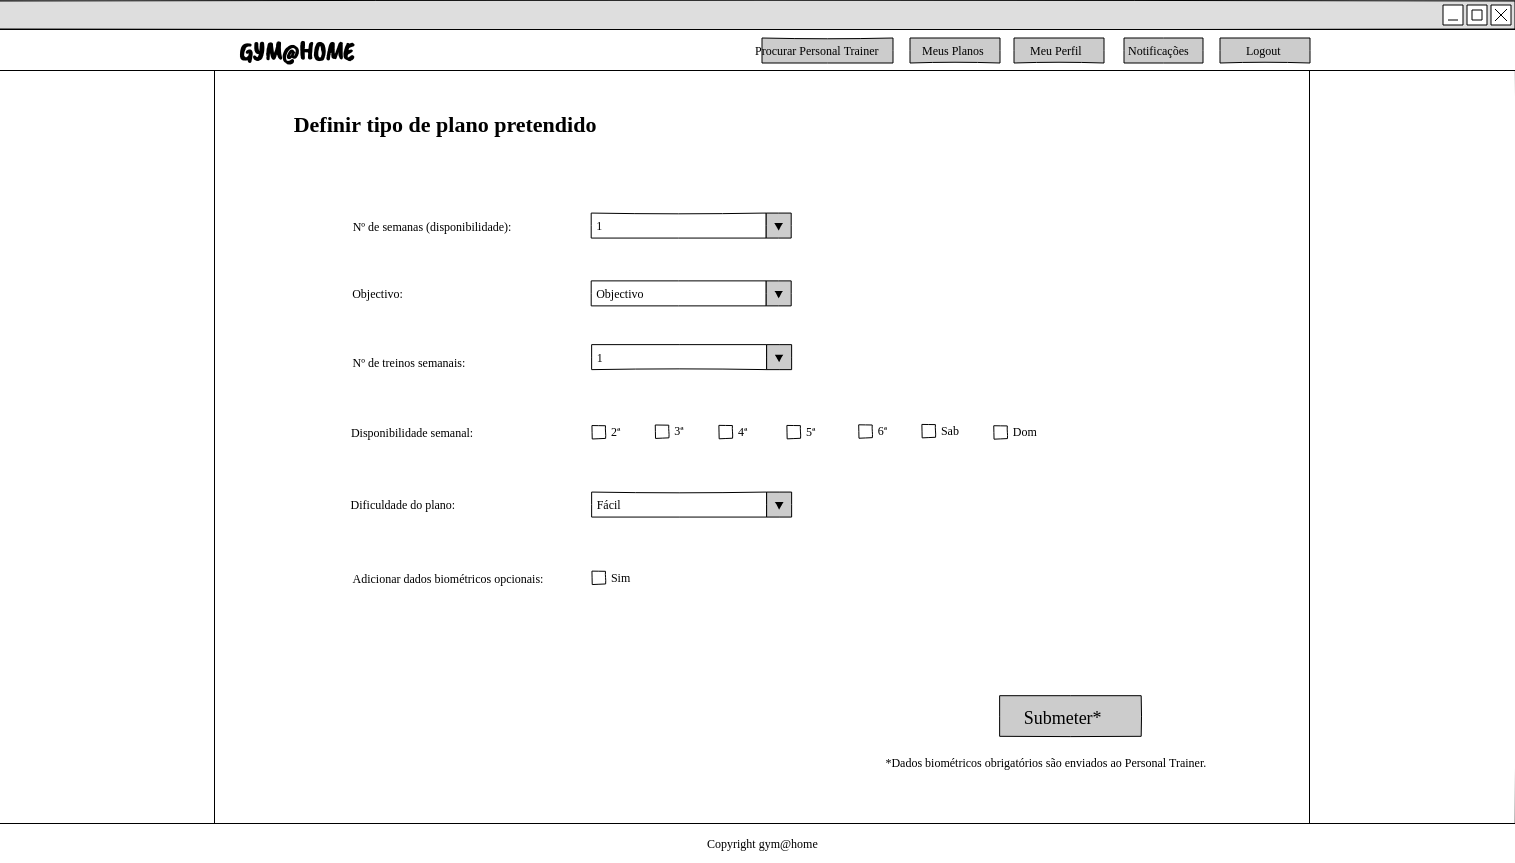
\includegraphics[scale=0.25]{images/mockups/cliente_formulrio.png}
    \caption{Mockup Preencher Pedido.}
    \label{fig:mockuppreencherpedido}
\end{figure}

\begin{figure}[H]
    \centering
    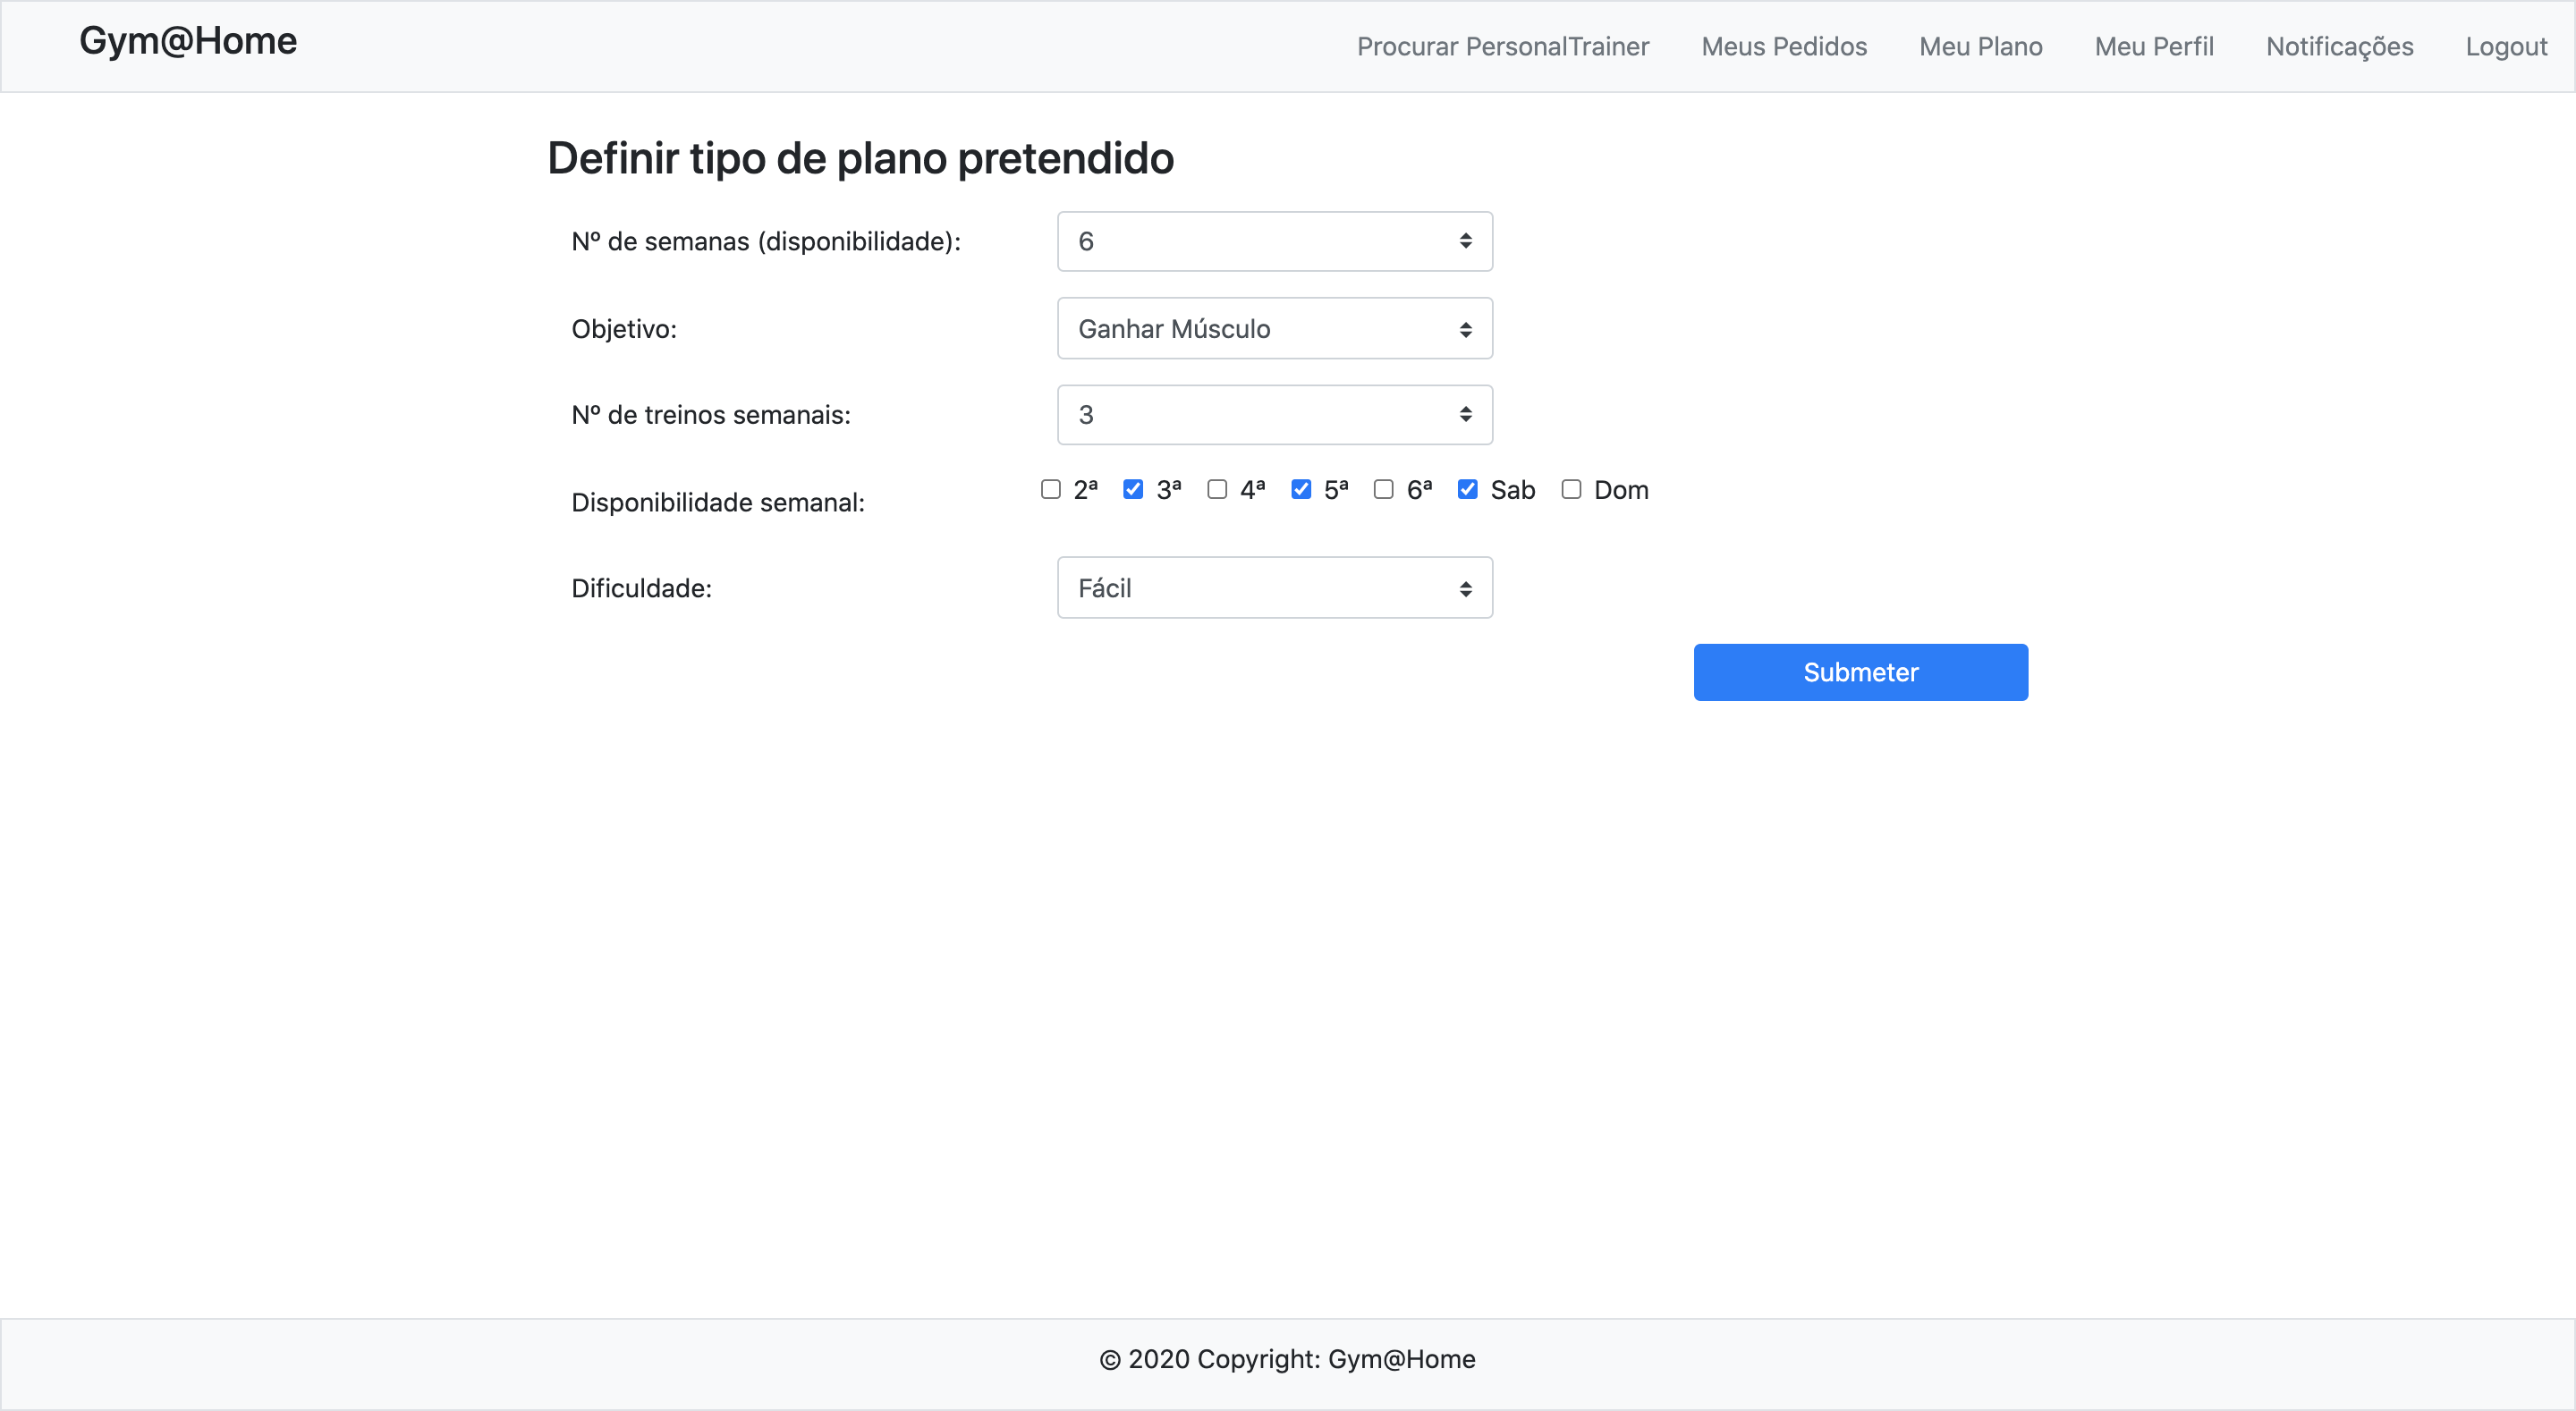
\includegraphics[scale=0.25]{images/interfaces/client_formulario.png}
    \caption{Interface Preencher Pedido.}
    \label{fig:interfacepreencherpedido}
\end{figure}

\subsubsection{Princípios de usabilidade}
\begin{itemize}
    \item \textbf{Synthesizability}: após a submissão do formulário/pedido de plano, vai ser redireccionado para a página que tem todos os pedidos enviados pelo Cliente, permitindo assim que o mesmo perceba o efeito da sua acção.
\end{itemize}

\subsubsection{Heurísticas de Normam}
\begin{itemize}
    \item \textbf{Error prevention}: Todos os inputs estão predefinidos, evitando assim erros por parte do Cliente.
    \item \textbf{Recognition rather than recall}: utilização de dropdowns permite que o utilizador não tenha que memorizar as opções existentes.
\end{itemize}

\subsection{Consultar Semana do plano}
\label{subsec:semana}

\subsubsection{Descrição}
\hspace{5mm} A mockup de visualização da Semana de um plano é comum a ambos o utilizadores, excepto que o Cliente contém um botão para avaliar o PT. Dessa forma, vamos apresentar a do Cliente, no entanto são praticamente semelhantes. 

\hspace{5mm} O Cliente consegue ver os workouts da semana, bem como verificar a sua condição física através dos seus dados biométricos. Na interface final foi acrescentada ainda uma barra do IMC com os valores de referência da OMS, informando assim o Cliente sobre o seu estado do IMC de forma mais intuitiva.

\hspace{5mm} Na tabela o Cliente pode seleccionar um workout tanto por realizar como realizado, sendo que no caso de já estar realizado não lhe é permitido realizar outra vez. Isto é possível para o Cliente poder ver as Tarefas que realizou em Workouts anteriores.

\hspace{5mm} Ainda nesta mockup contém a funcionalidade de avaliar o PT, para o cálculo da sua classificação.

\begin{figure}[H]
    \centering
    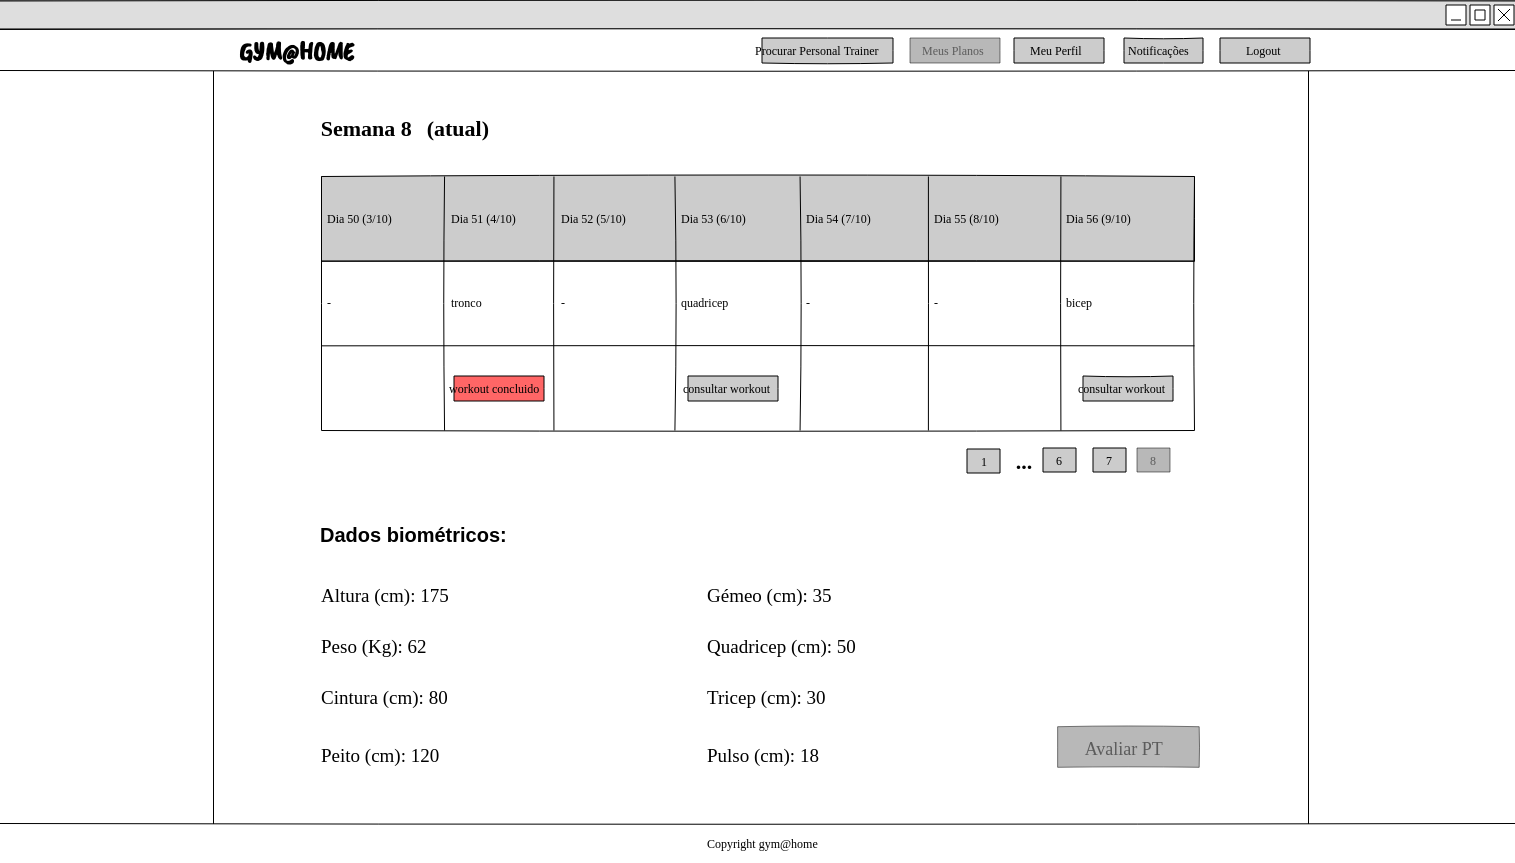
\includegraphics[scale=0.25]{images/mockups/cliente_meus_planos_semana_8_atual.png}
    \caption{Mockup Semana.}
    \label{fig:mockupsemana}
\end{figure}

\begin{figure}[H]
    \centering
    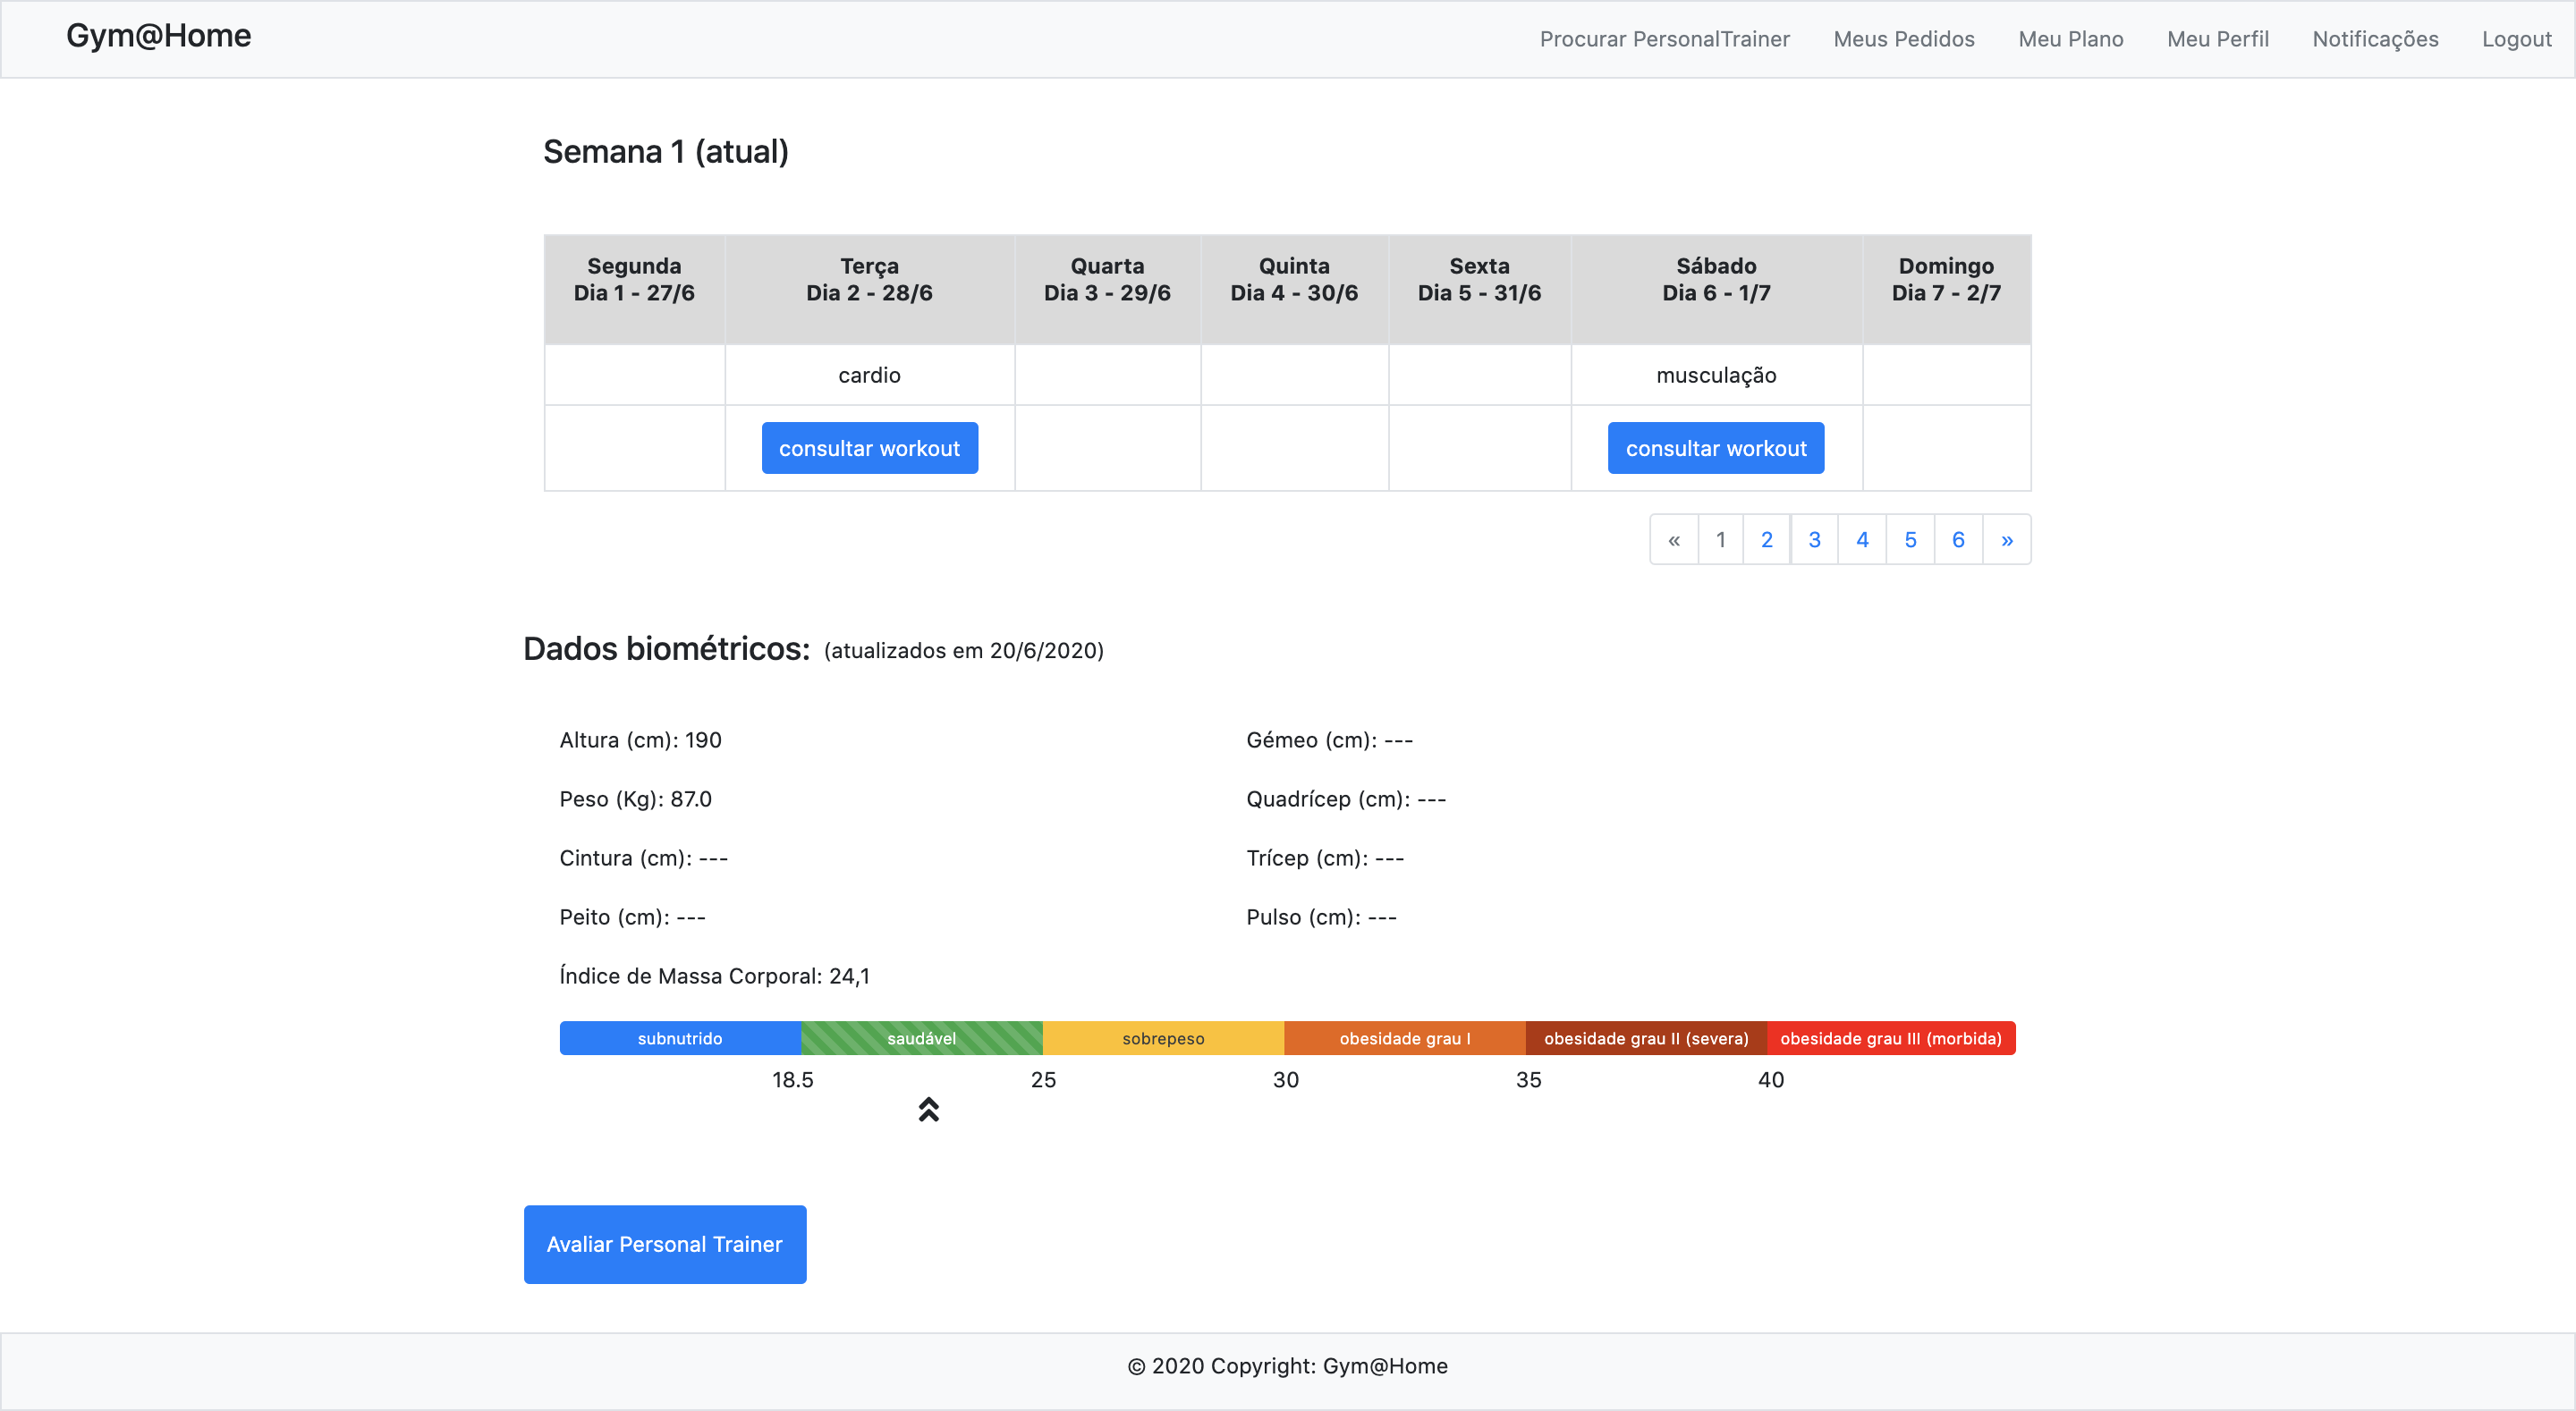
\includegraphics[scale=0.25]{images/interfaces/client_semana.png}
    \caption{Interface Semana.}
    \label{fig:interfacesemana}
\end{figure}

\subsubsection{Princípios de Usabilidade}
\begin{itemize}
    \item \textbf{Observability}: Mais especificamente \textbf{Browsability} pois o Cliente consegue navegar entre as várias semanas do seu plano.
    \item \textbf{Familiarity}: utilizou-se o formato semanal \textbf{comum}/\textbf{padrão} em horários e calendários, visto que é mais familiar aos utilizadores.
    \item \textbf{Generalizability} e \textbf{Consistency}: visto que utilizou-se a mesma estrutura tanto para a consulta pelo Cliente, bem como pelo PT, apesar de terem algumas diferenças, manteve-se a estrutura semanal, bem como os dados biométricos, excepto o botão de avaliação do PT, que não faz sentido no lado do PT.
\end{itemize}

\subsubsection{Heurísticas de Normam}
\begin{itemize}
    \item \textbf{Visibility of system status}: o utilizador conhece o estado da aplicação, como por exemplo, os \textbf{workouts} que já foram feitos, aparecem com uma cor diferente. 
    \item \textbf{Recognition rather than recall}: Os dados biométricos do Cliente são ilustrados durante a visualização da semana para o Cliente não ter de se lembrar de quais eram os valores dos dados biométricos.
    \item \textbf{Consistency and standards}: tal como foi dito em relação à \textbf{Familiarity}, sobre a estrutura semana usada, também se aplica a esta heurística relacionada com consistência e padrões.
\end{itemize}

\subsection{Consultar Workout}
\label{subsec:workout}

\subsubsection{Descrição}
\hspace{5mm} Da mesma forma que o anterior, este mockup também é bastante semelhante a ambos os utilizadores, pelo que apresentar-se-á apenas a view do Cliente. Nesta mockup o Cliente vê uma Tarefa de cada vez, com a listagem das séries e toda a informação necessário sobre a Tarefa. Aqui pode avançar e recuar nas tarefas, sendo que na última Tarefa do Workout pode terminar o Workout.

\begin{figure}[H]
    \centering
    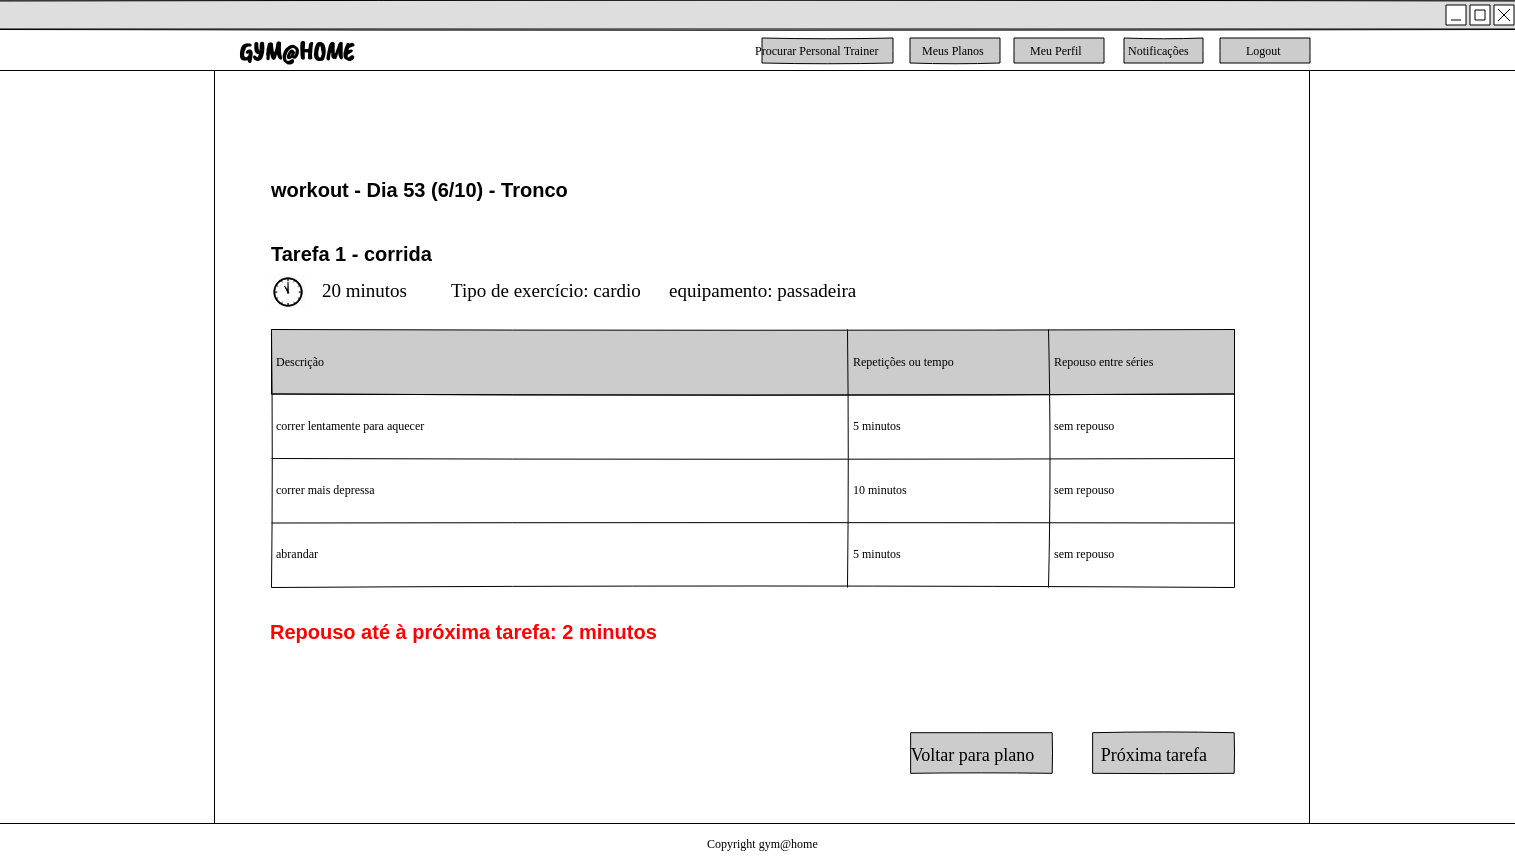
\includegraphics[scale=0.25]{images/mockups/cliente_plano_tarefa_1.png}
    \caption{Mockup Workout.}
    \label{fig:mockupworkout}
\end{figure}

\begin{figure}[H]
    \centering
    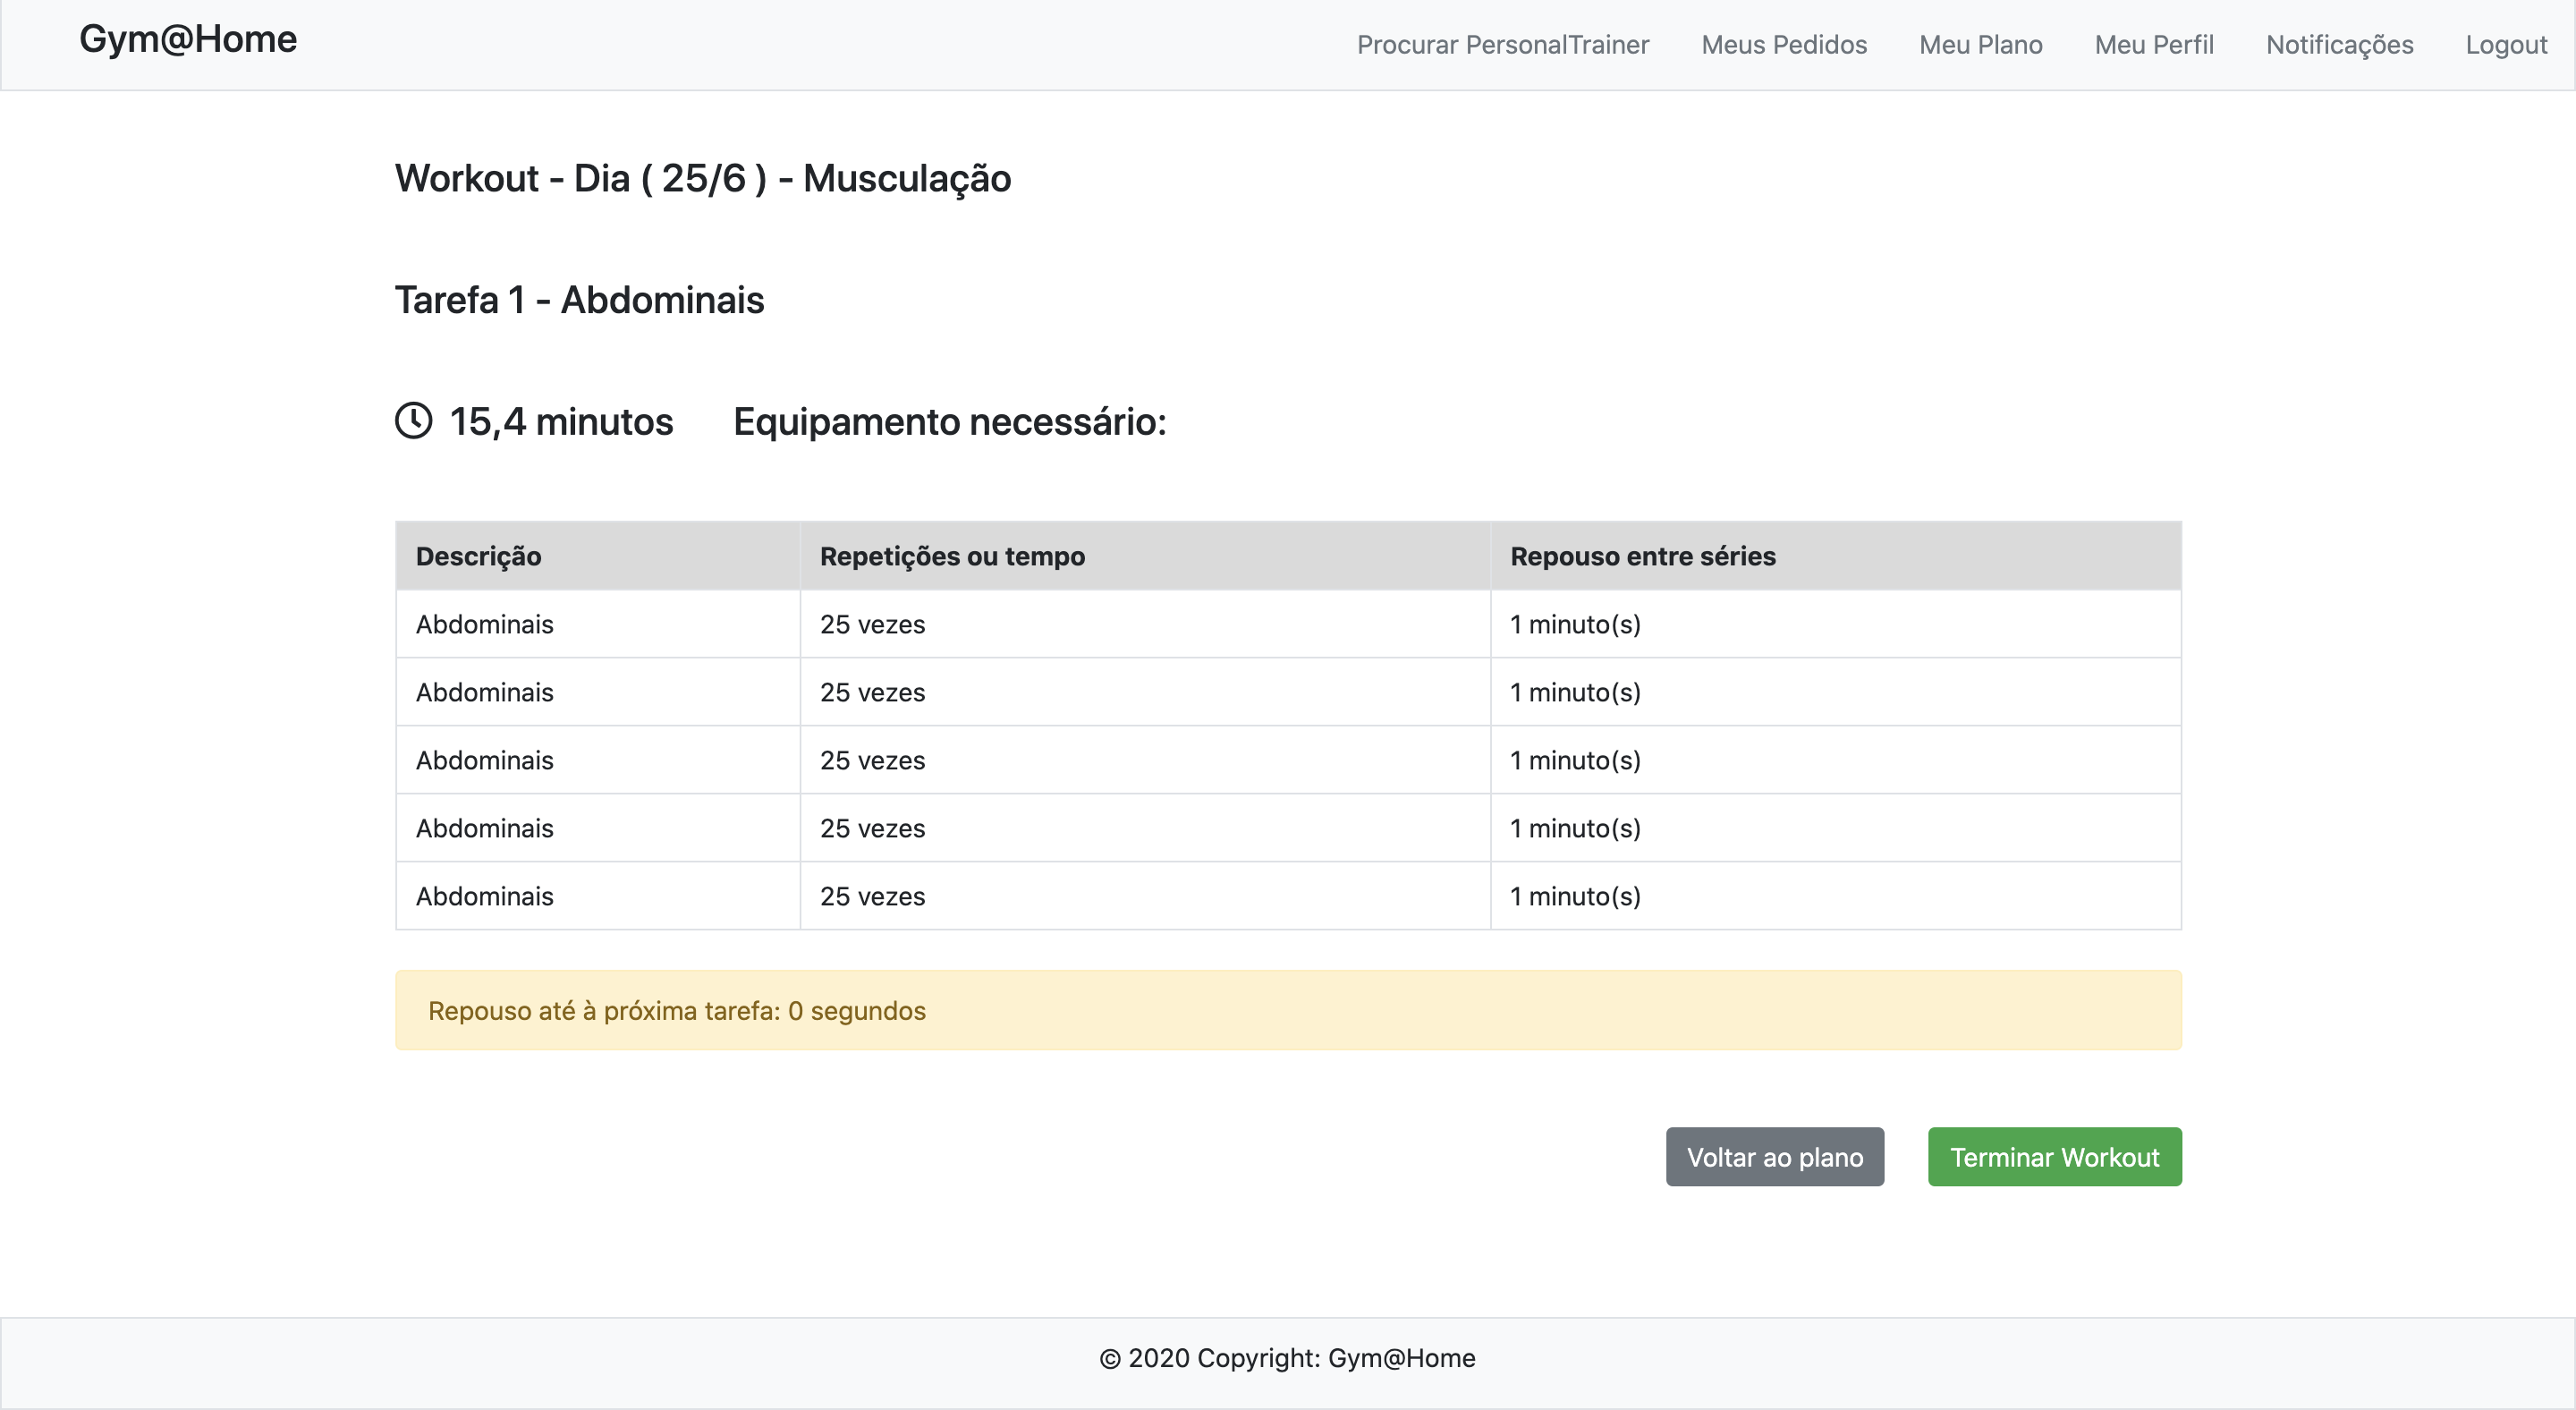
\includegraphics[scale=0.25]{images/interfaces/client_workout.png}
    \caption{Interface Workout.}
    \label{fig:interfaceworkout}
\end{figure}

\subsubsection{Princípios de usabilidade}
\begin{itemize}
    \item \textbf{Observability}: Mais especificamente \textbf{Browsability} pois o Cliente consegue navegar entre as várias tarefas de um workout.
    
    \item \textbf{Generalizability} e \textbf{Consistency}: visto que utilizou-se a mesma estrutura tanto para a consulta pelo Cliente, bem como pelo PT, apesar de terem algumas diferenças, manteve-se a estrutura tabelar das séries de uma tarefa, bem como as informações da tarefa, considerando-se assim que torna-se genérica para ambos os utilizadores.
\end{itemize}

\subsubsection{Heurísticas de Normam}
\begin{itemize}
    \item \textbf{Recognition rather than recall}: as informações sobre o dia da semana e a definição do workout são passadas para esta view para que o cliente/PT não necessitem de memorizar.
\end{itemize}

\subsection{Pedidos enviados pelo Cliente}
\label{subsec:pedidos}

\subsubsection{Descrição}
\hspace{5mm} A interface Pedidos enviados pelo Cliente foi adicionada posteriormente ao desenho das mockups, pelo que só existe a interface final. Nesta interface o Cliente poderá ver todos os pedidos que já realizou, sendo apresentadas todas as informações do pedido, tais como o seu estado (aceite, rejeitado ou pedente), nome do PT, dados do formulário preenchido e ainda a possibilidade de ver o perfil do PT ao qual o pedido foi direccionado.

\begin{figure}[H]
    \centering
    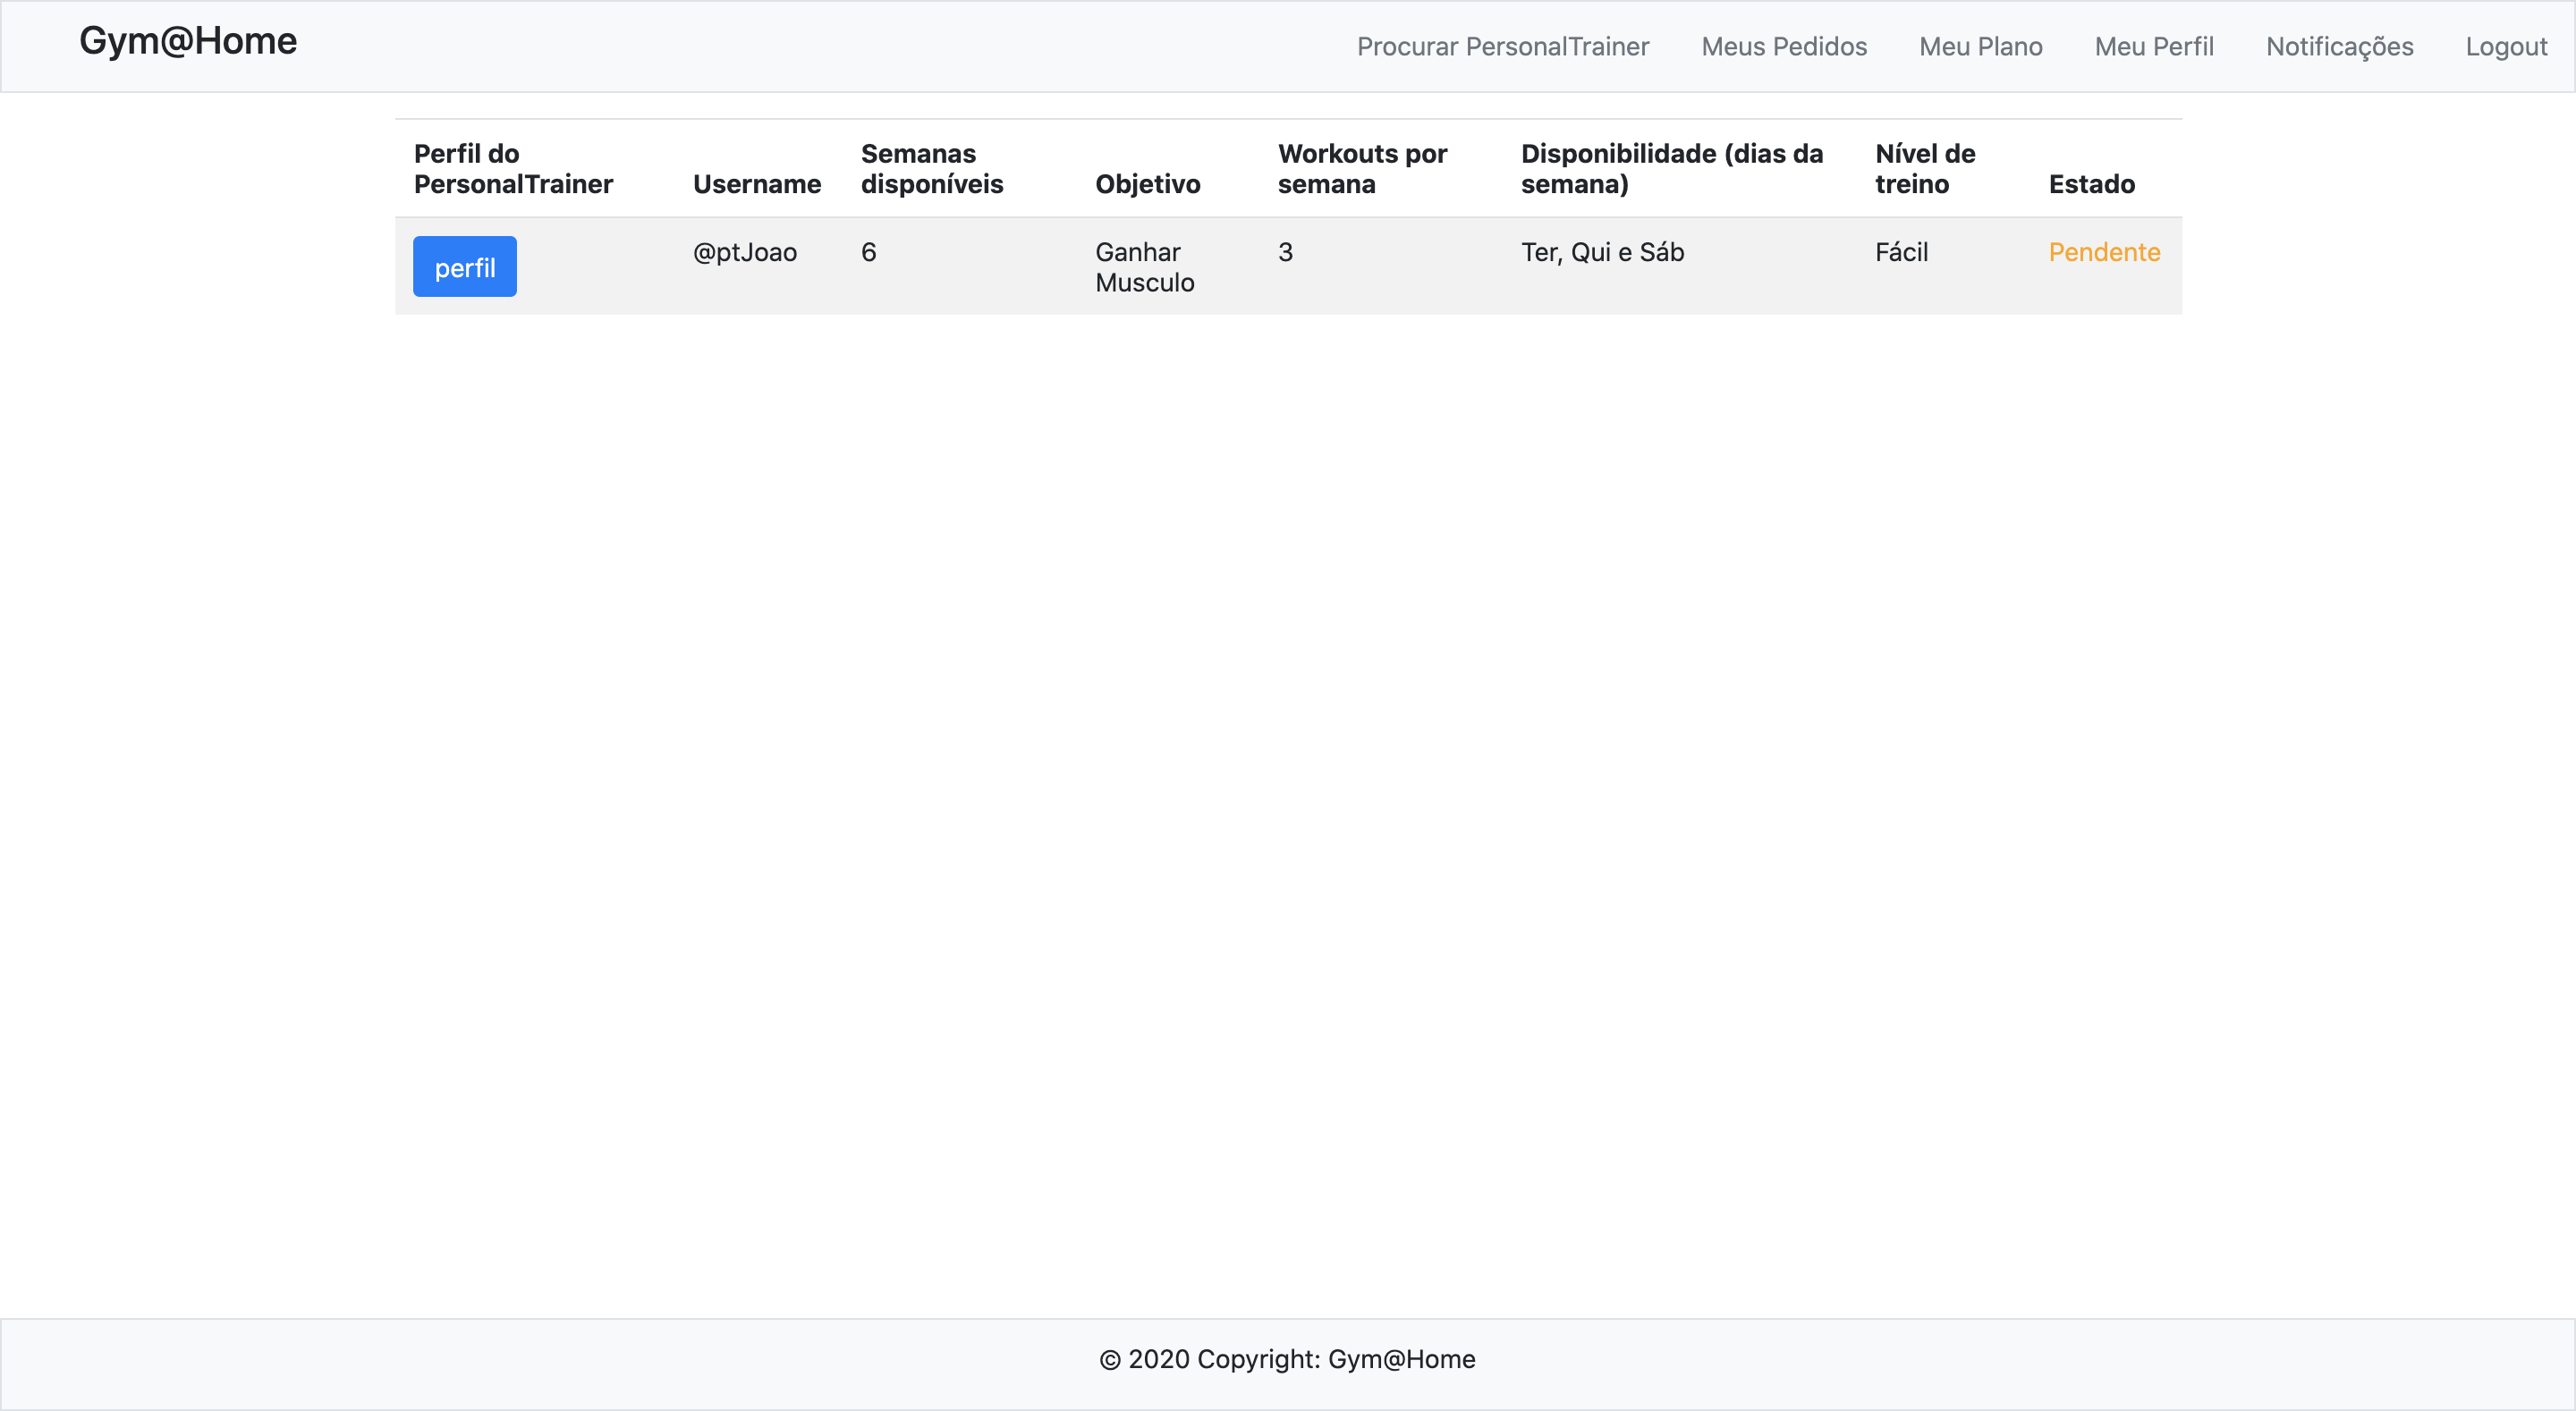
\includegraphics[scale=0.25]{images/interfaces/client_meus_pedidos.png}
    \caption{Interface Pedidos.}
    \label{fig:interfacepedidos}
\end{figure}

\subsubsection{Princípios de usabilidade}
\begin{itemize}
    \item \textbf{Synthesizability}: a acção possível nesta interface consiste em consultar o perfil do PT, pelo que após clicar no botão "perfil", aparece um pop-up com as informações do mesmo, ou seja, o cliente consegue perceber o efeito das suas acções.
    \item \textbf{Generalizability} e \textbf{Consistency}: o PT também contem uma interface para ver os pedidos enviados para o mesmo, que a nível de estrutura pode-se considerar bastante semelhante, difere apenas no conteúdos de algumas colunas, pelo que se pode considerar que se trata de uma interface genérica no sistema. 
    \item \textbf{Observability}: esta interface pode aumentar bastante o número de linhas da tabela, no entanto cada linha tem os botões para as acções desse pedido, o que significa que se houvesse uma tabela gigante, as acções possíveis estariam lá, não necessitando de subir a página ou outra forma para encontrar os botões. No entanto o grupo reconhece que aqui também seria um bom candidato a paginação, não sendo possível implementar face à falta de tempo, mas será uma boa actualização no futuro.
\end{itemize}

\subsubsection{Heurísticas de Normam}
\begin{itemize}
    \item \textbf{Recognition rather than recall}: o cliente não precisa de memorizar o que preencheu no formulário quando enviou o pedido, pois pode consultar na tabela esses mesmos campos.
    \item \textbf{Flexibility and efficiency of use}: o botão "perfil", que mostra as informações do PT torna esse processo de consulta mais \textbf{eficiente}, como uma espécie de atalho.
\end{itemize}

\subsection{Avaliar PT}
\label{subsec:avaliarpt}

\subsubsection{Descrição}
\hspace{5mm} A qualquer momento o Cliente pode avaliar o PT pelo seu trabalho, sendo pedido uma classificação de 1 a 5 estrelas, estas avaliações serão usadas posteriormente como parâmetro para escolher ou não um PT.

\begin{figure}[H]
    \centering
    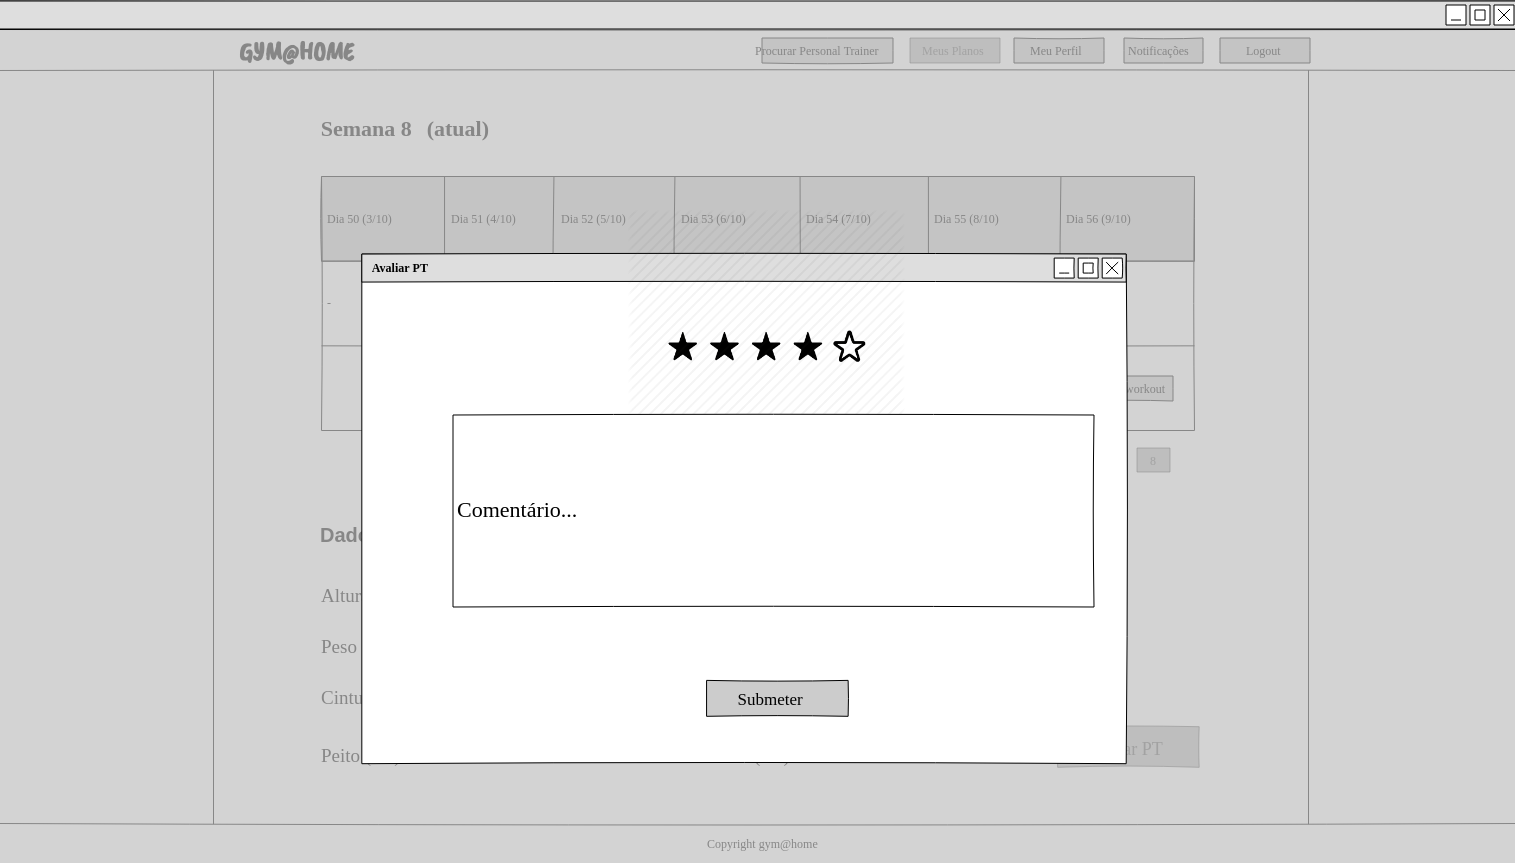
\includegraphics[scale=0.25]{images/mockups/cliente_avaliar_pt.png}
    \caption{Mockup Avaliar PT.}
    \label{fig:mockupavaliarpt}
\end{figure}

\begin{figure}[H]
    \centering
    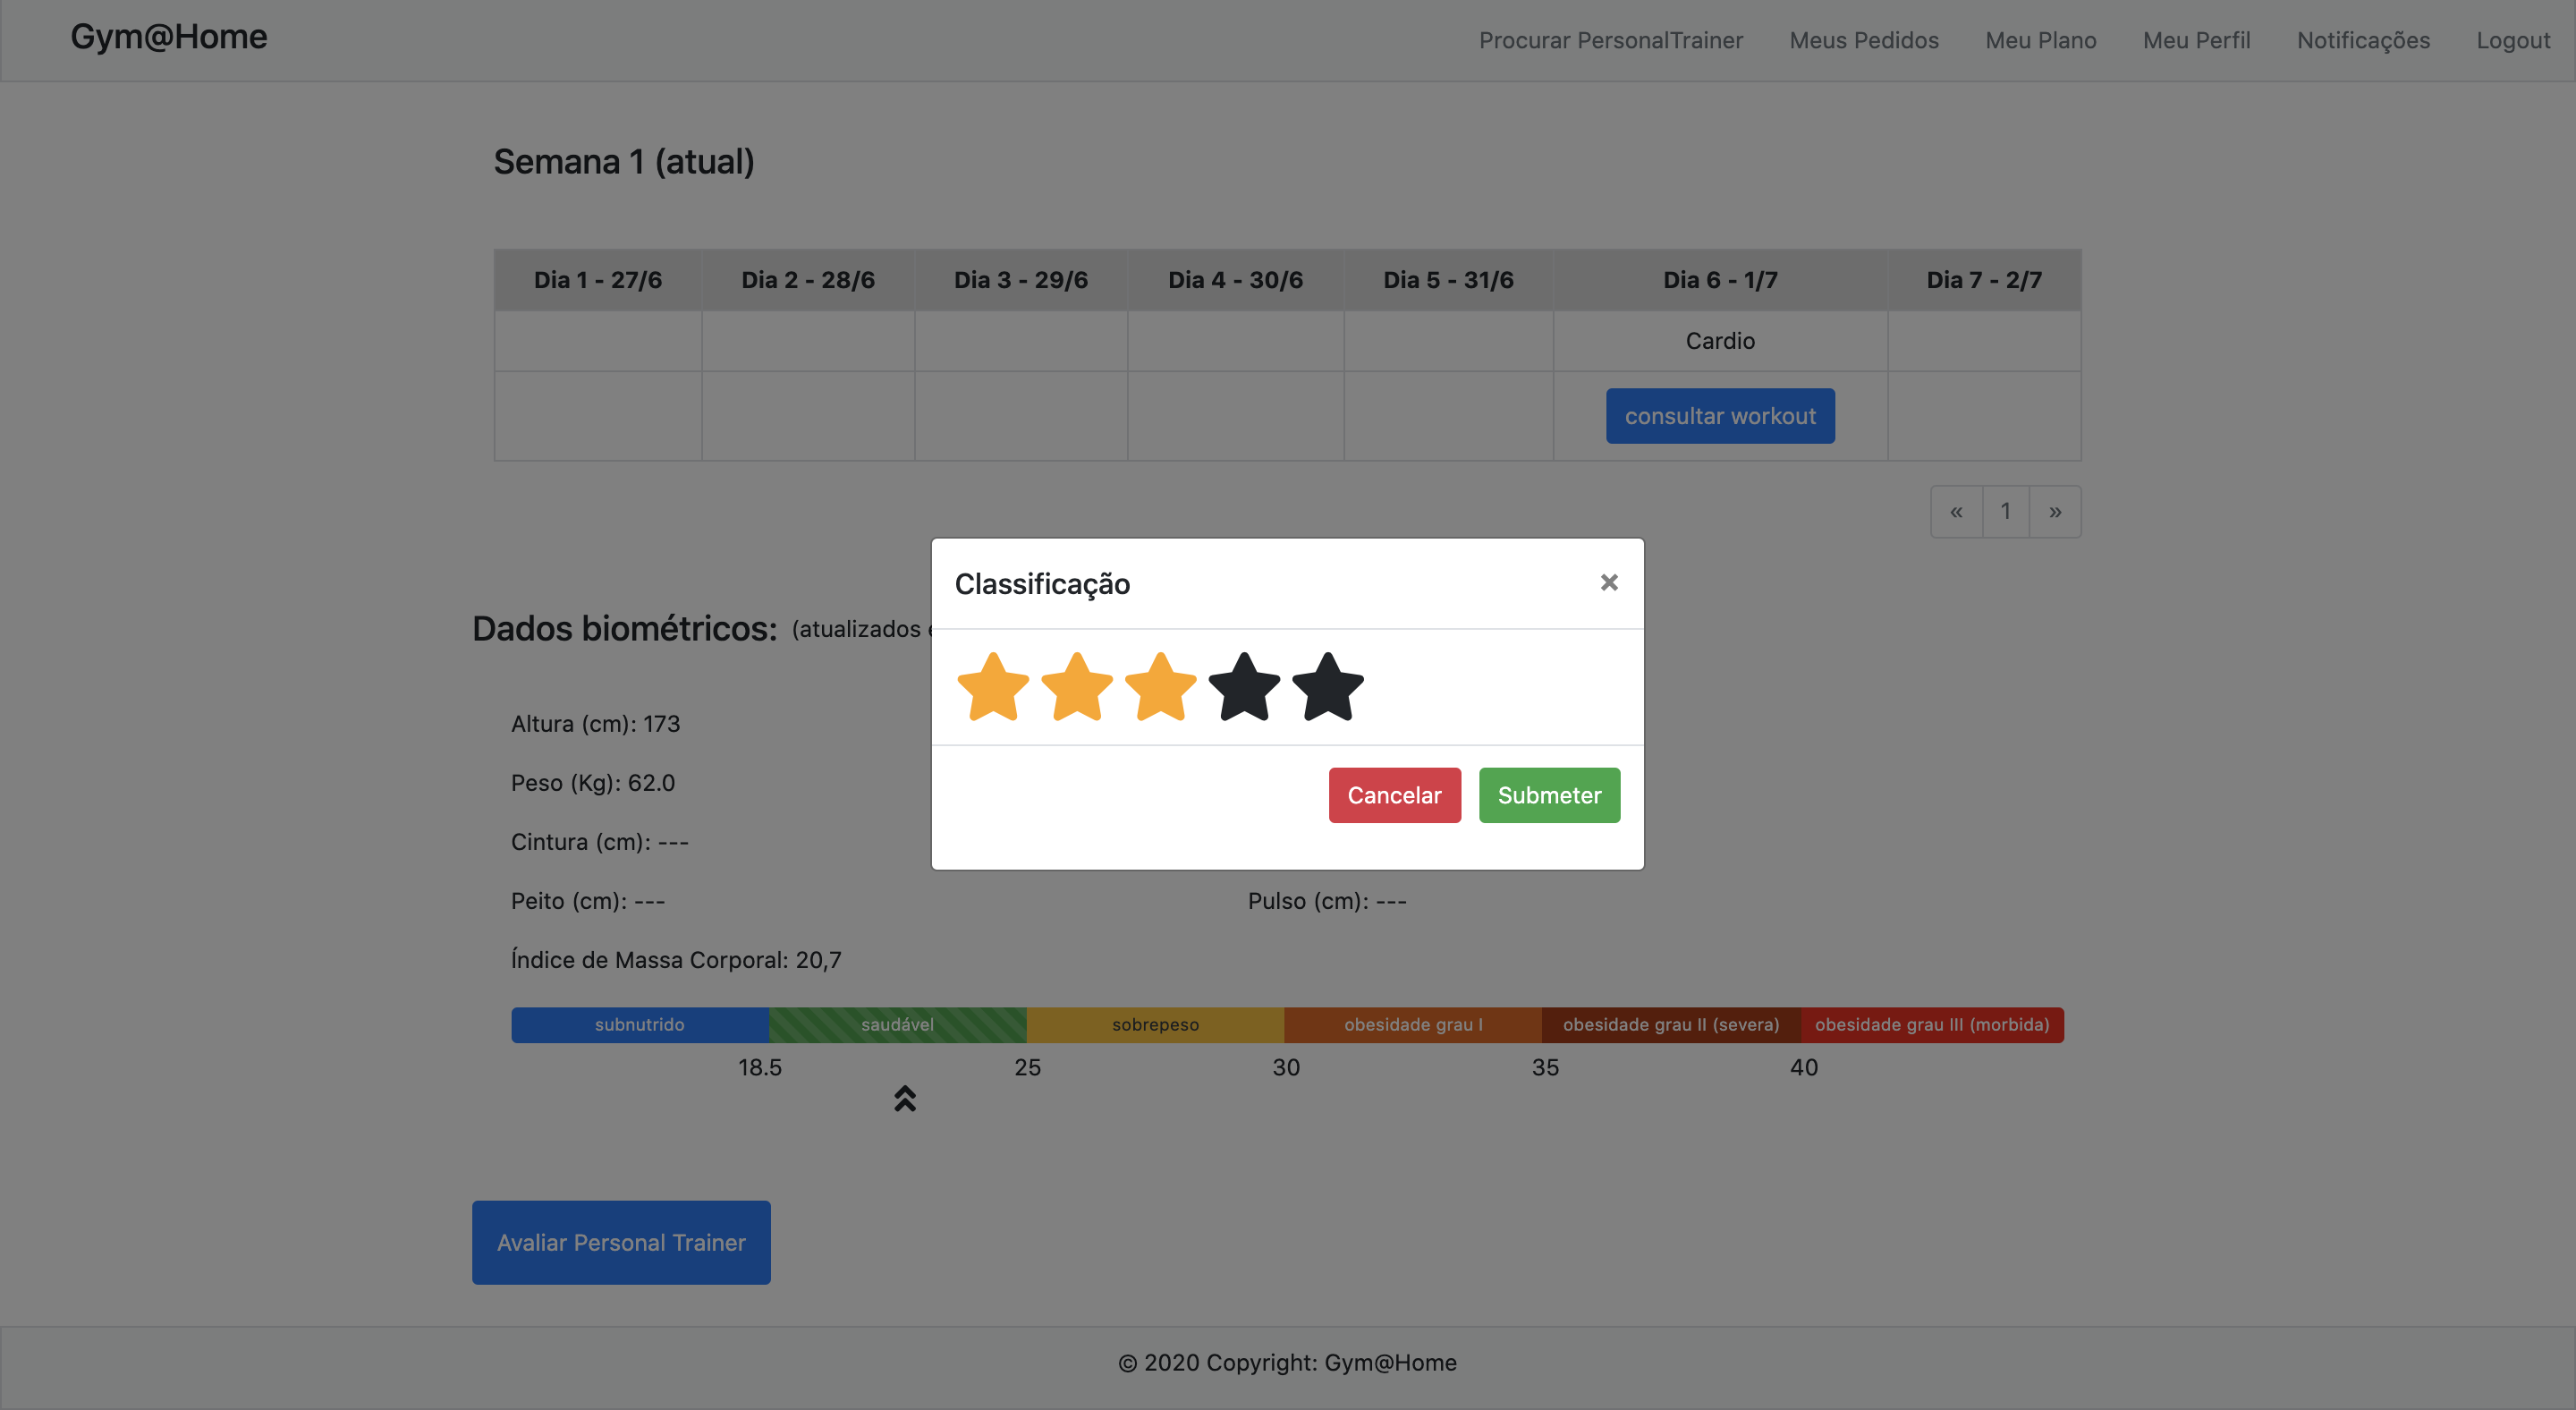
\includegraphics[scale=0.25]{images/interfaces/client_avaliar_pt.png}
    \caption{Interface Avaliar PT.}
    \label{fig:interfaceavaliarpt}
\end{figure}

\subsubsection{Princípios de usabilidade}
\begin{itemize}
    \item \textbf{Familiarity} e \textbf{Consistency}: usou-se uma forma padrão para as avaliações, através de cinco estrelas onde o utilizador selecciona.
\end{itemize}

\subsubsection{Heurísticas de Normam}
\begin{itemize}
    \item \textbf{Error prevetion}: a avaliação é inicializada com pelo menos uma estrela seleccionada, para evitar que o utilizador pudesse enviar zero estrelas, visto que a escala vai de um a cinco.
    \item \textbf{Consistency and standards}: tal como foi dito anteriormente, segue os princípios de \textbf{Familiarity} e \textbf{Consistency}, pelo que significa que também segue esta heurística relacionada com \textbf{padrões}.
\end{itemize}

%--------------------------------------------------------------------------%

\section{Interfaces PTs}
\label{sec:mockupspts}

\subsection{Registar PT}
\label{subsec:registarpt}

\subsubsection{Descrição}
\hspace{5mm} Tal como no registo Cliente são pedidos alguns dados obrigatórios, sendo que o PT não tem dados opcionais.

\begin{figure}[H]
    \centering
    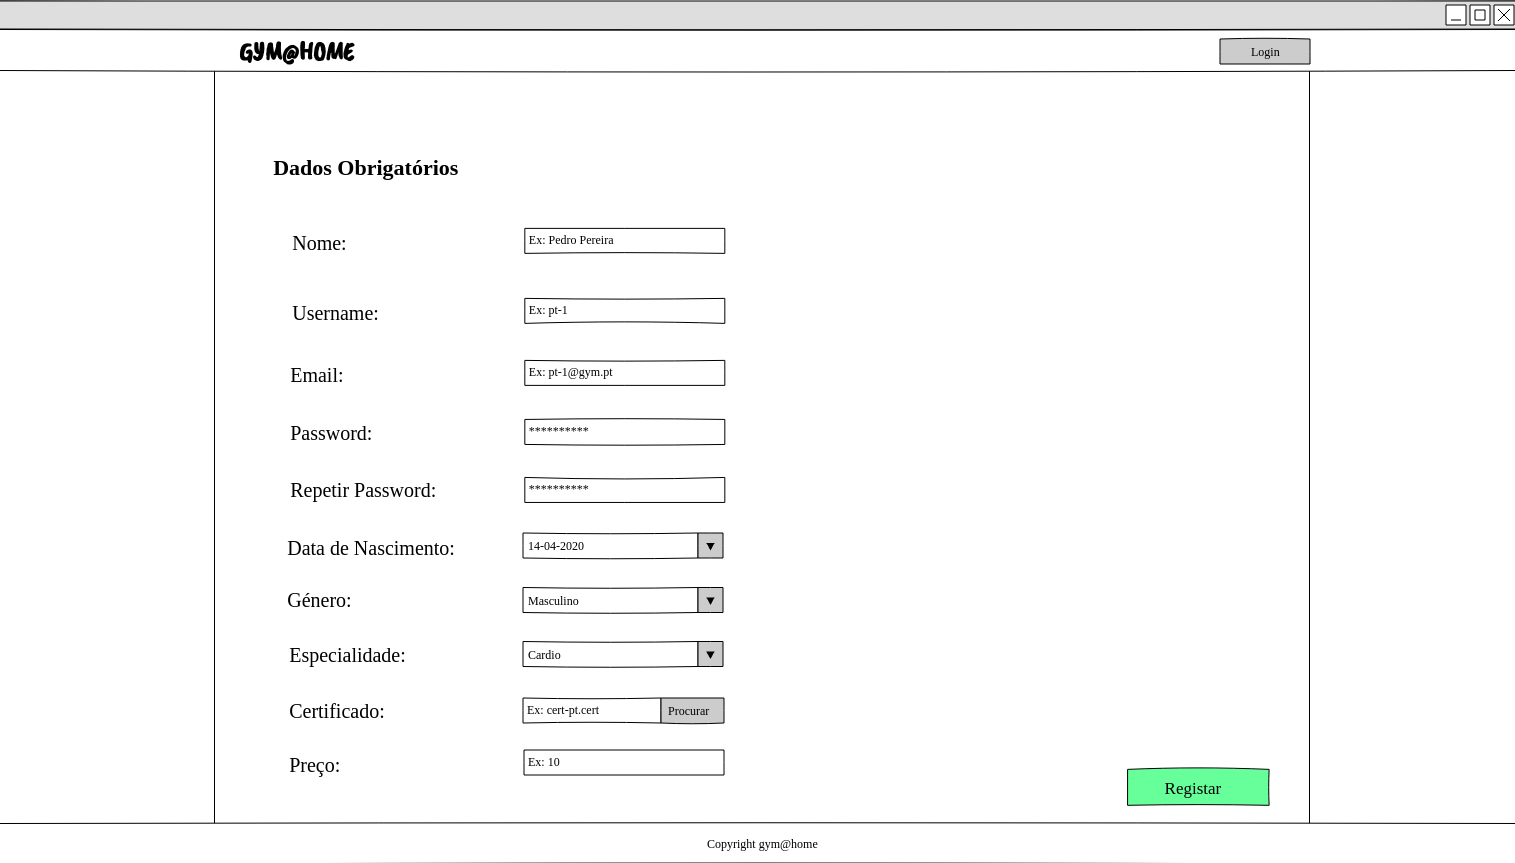
\includegraphics[scale=0.25]{images/mockups/pt_registo.png}
    \caption{Mockup Registar PT.}
    \label{fig:mockupregistarpt}
\end{figure}

\begin{figure}[H]
    \centering
    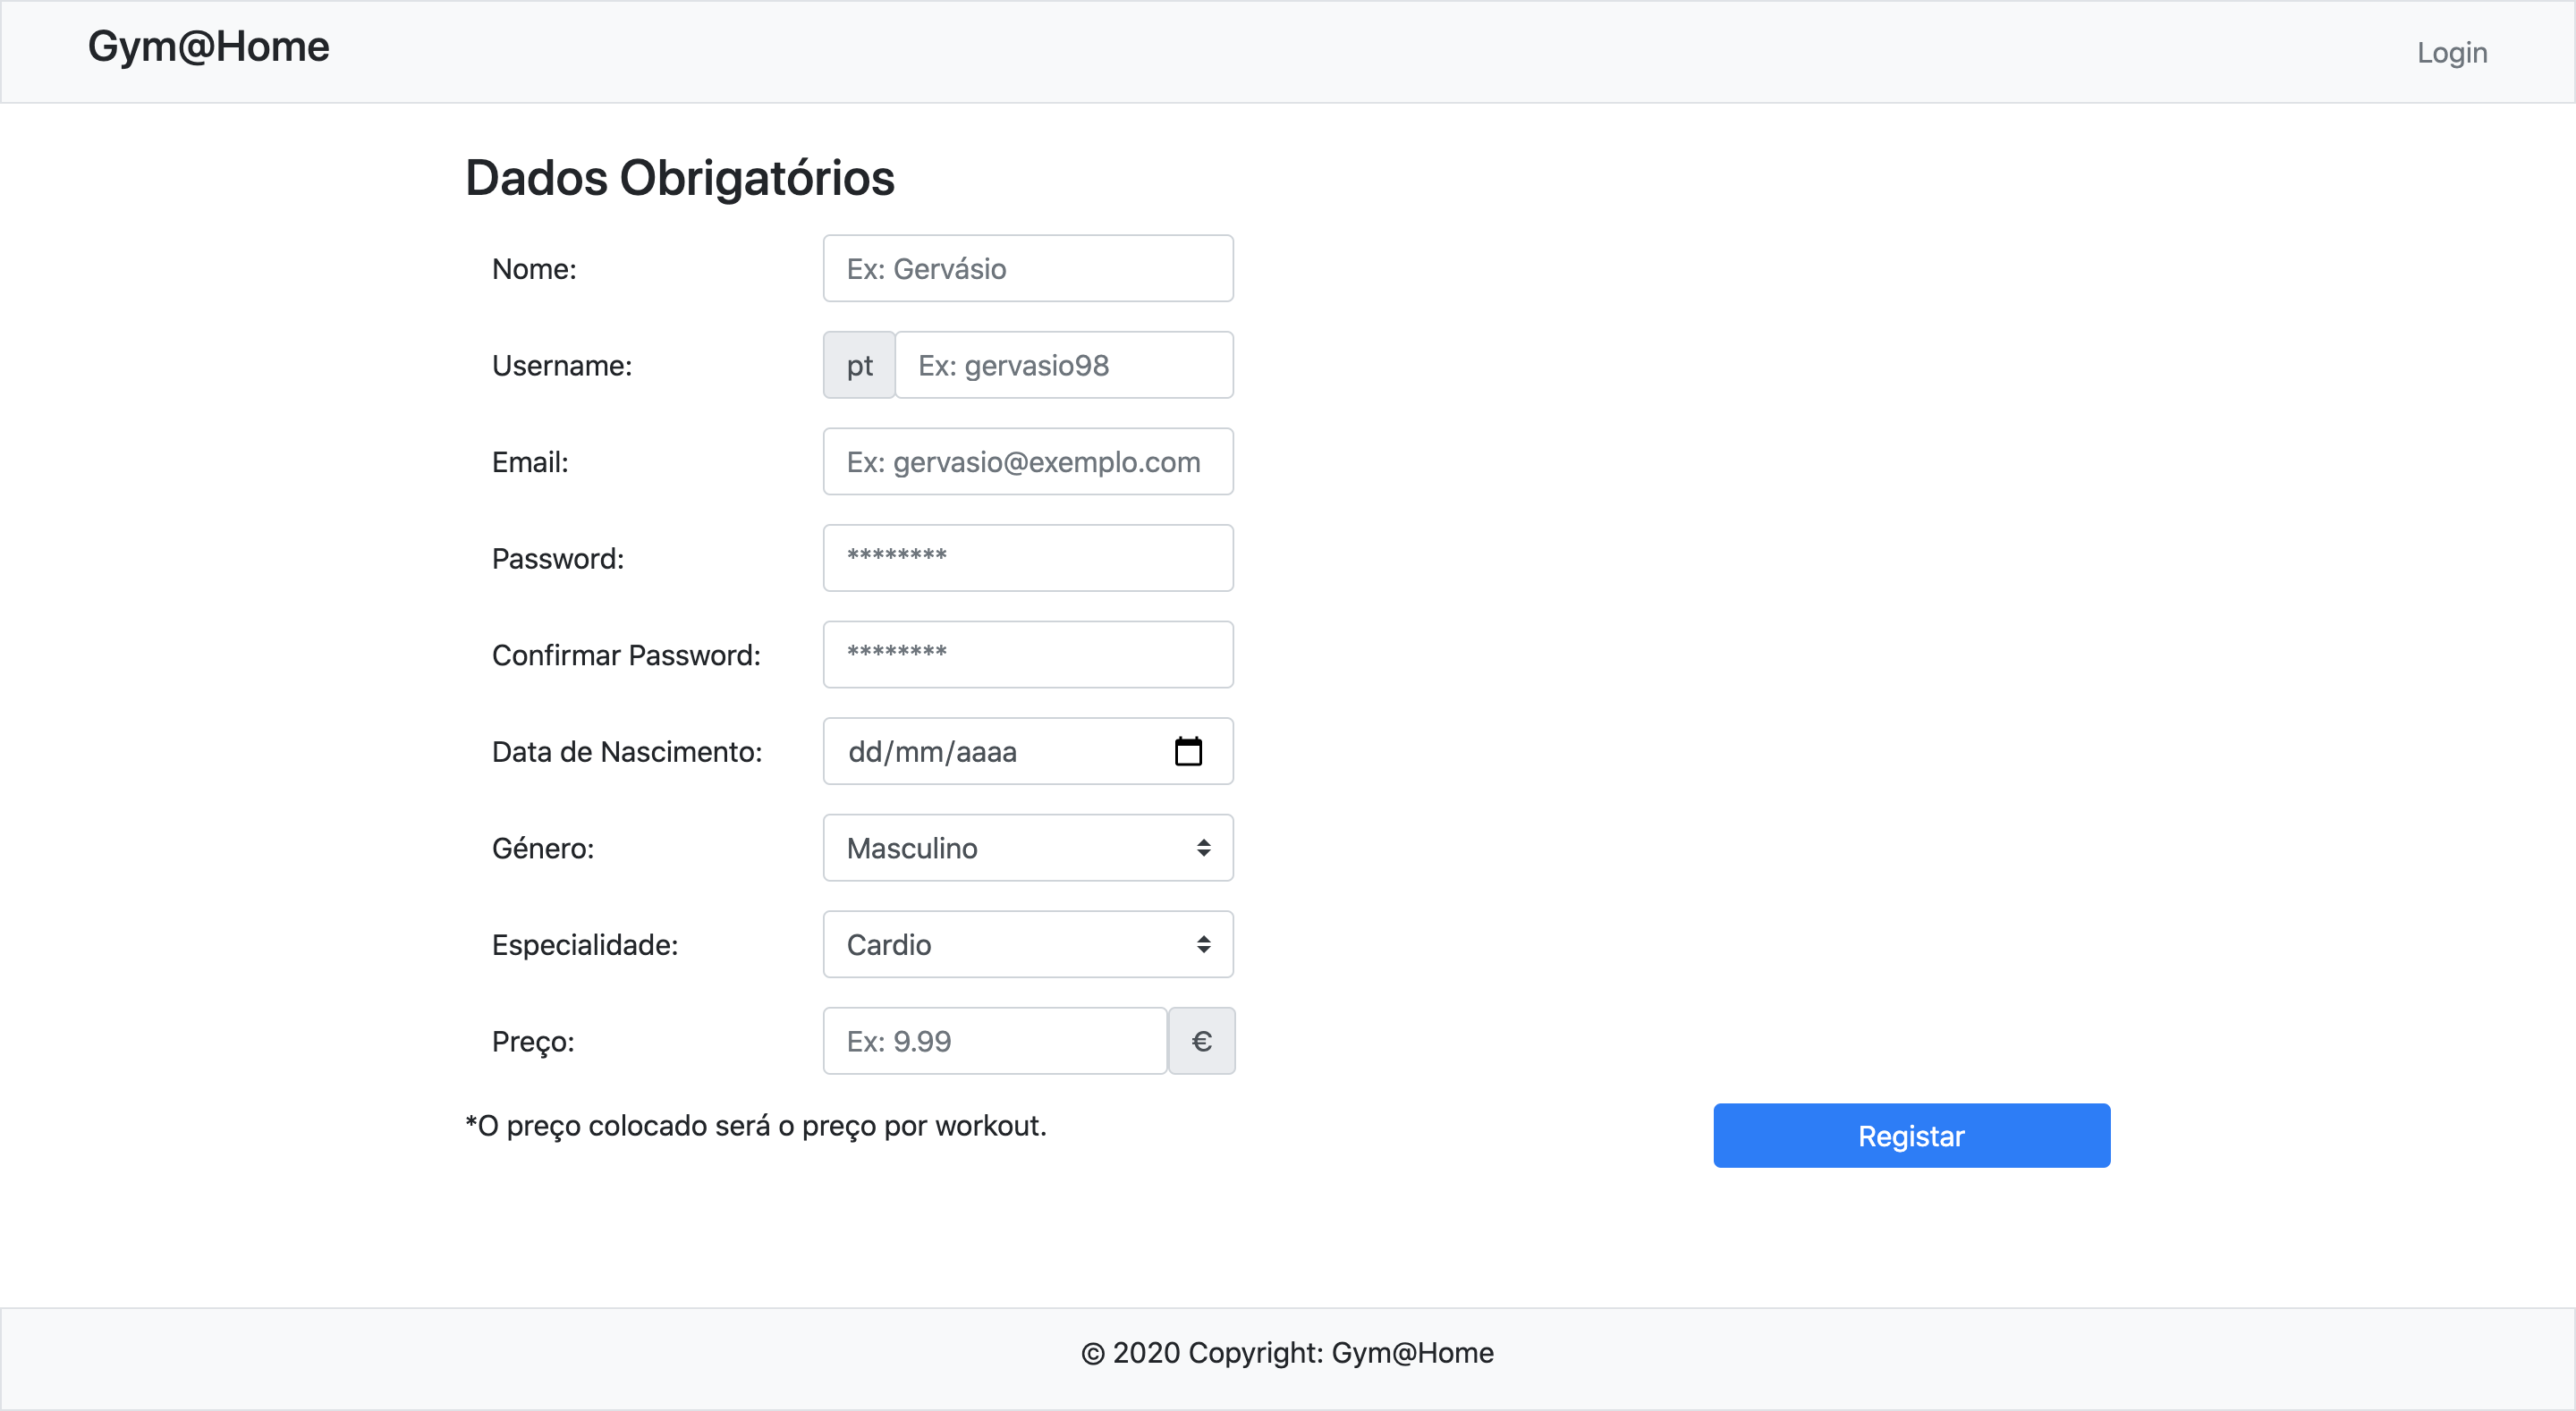
\includegraphics[scale=0.25]{images/interfaces/pt_register.png}
    \caption{Interface Registar PT.}
    \label{fig:interfaceregistarpt}
\end{figure}

\subsubsection{Princípios de Usabilidade}
\begin{itemize}
    \item \textbf{Familiarity} e \textbf{Consistency}: Colocar a "Data de Nascimento" é feito através de um calendário, pelo que o PT como ser humano está mais familiarizado a utilizar.
\end{itemize}

\subsubsection{Heurísticas de Normam}
\begin{itemize}
    \item \textbf{Error prevention}: Todos os inputs numéricos aceitam apenas números, o "Género" e "Especialidade" apenas permite os valores dos dropdowns, a "Data de Nascimento" apenas permite datas seleccionadas pelo calendário e o "Email" apenas aceita um email (tem de conter o @).
    \item \textbf{Consistency and standards}: tal como foi dito anteriormente, segue os princípios de \textbf{Familiarity} e \textbf{Consistency}, pelo que significa que também segue esta heurística relacionada com \textbf{padrões}.
    \item \textbf{Flexibility and efficiency of use}: visto que após ser feito o registo, faz-se o login automático, sendo mais \textbf{eficiente} para o cliente.
\end{itemize}

\subsection{PT consulta/edita o próprio perfil}
\label{subsec:perfilptbypt}

\subsubsection{Descrição}
\hspace{5mm} Do mesmo modo que o Cliente o PT pode visualizar e editar o seu perfil através desta mockup. Também nesta interface final, o botão de "Salvar Alterações" foi deslocado para o cimo da página para facilitar a sua visualização em ecrãs mais pequenos.

\begin{figure}[H]
    \centering
    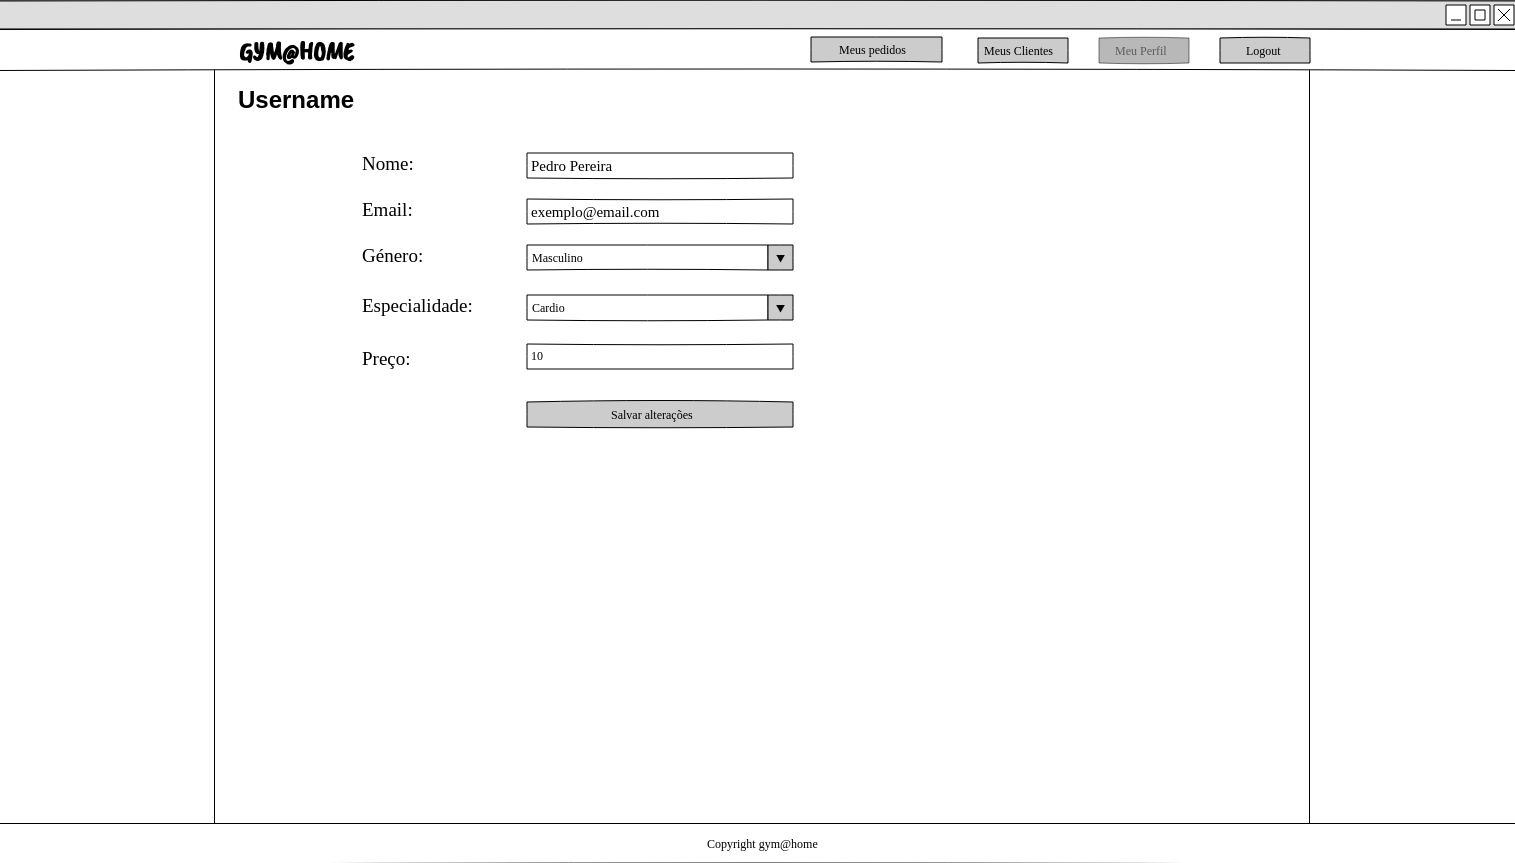
\includegraphics[scale=0.25]{images/mockups/pt_meu_perfil.png}
    \caption{Mockup Perfil PT visto pelo próprio.}
    \label{fig:mockupperfilptbypt}
\end{figure}

\begin{figure}[H]
    \centering
    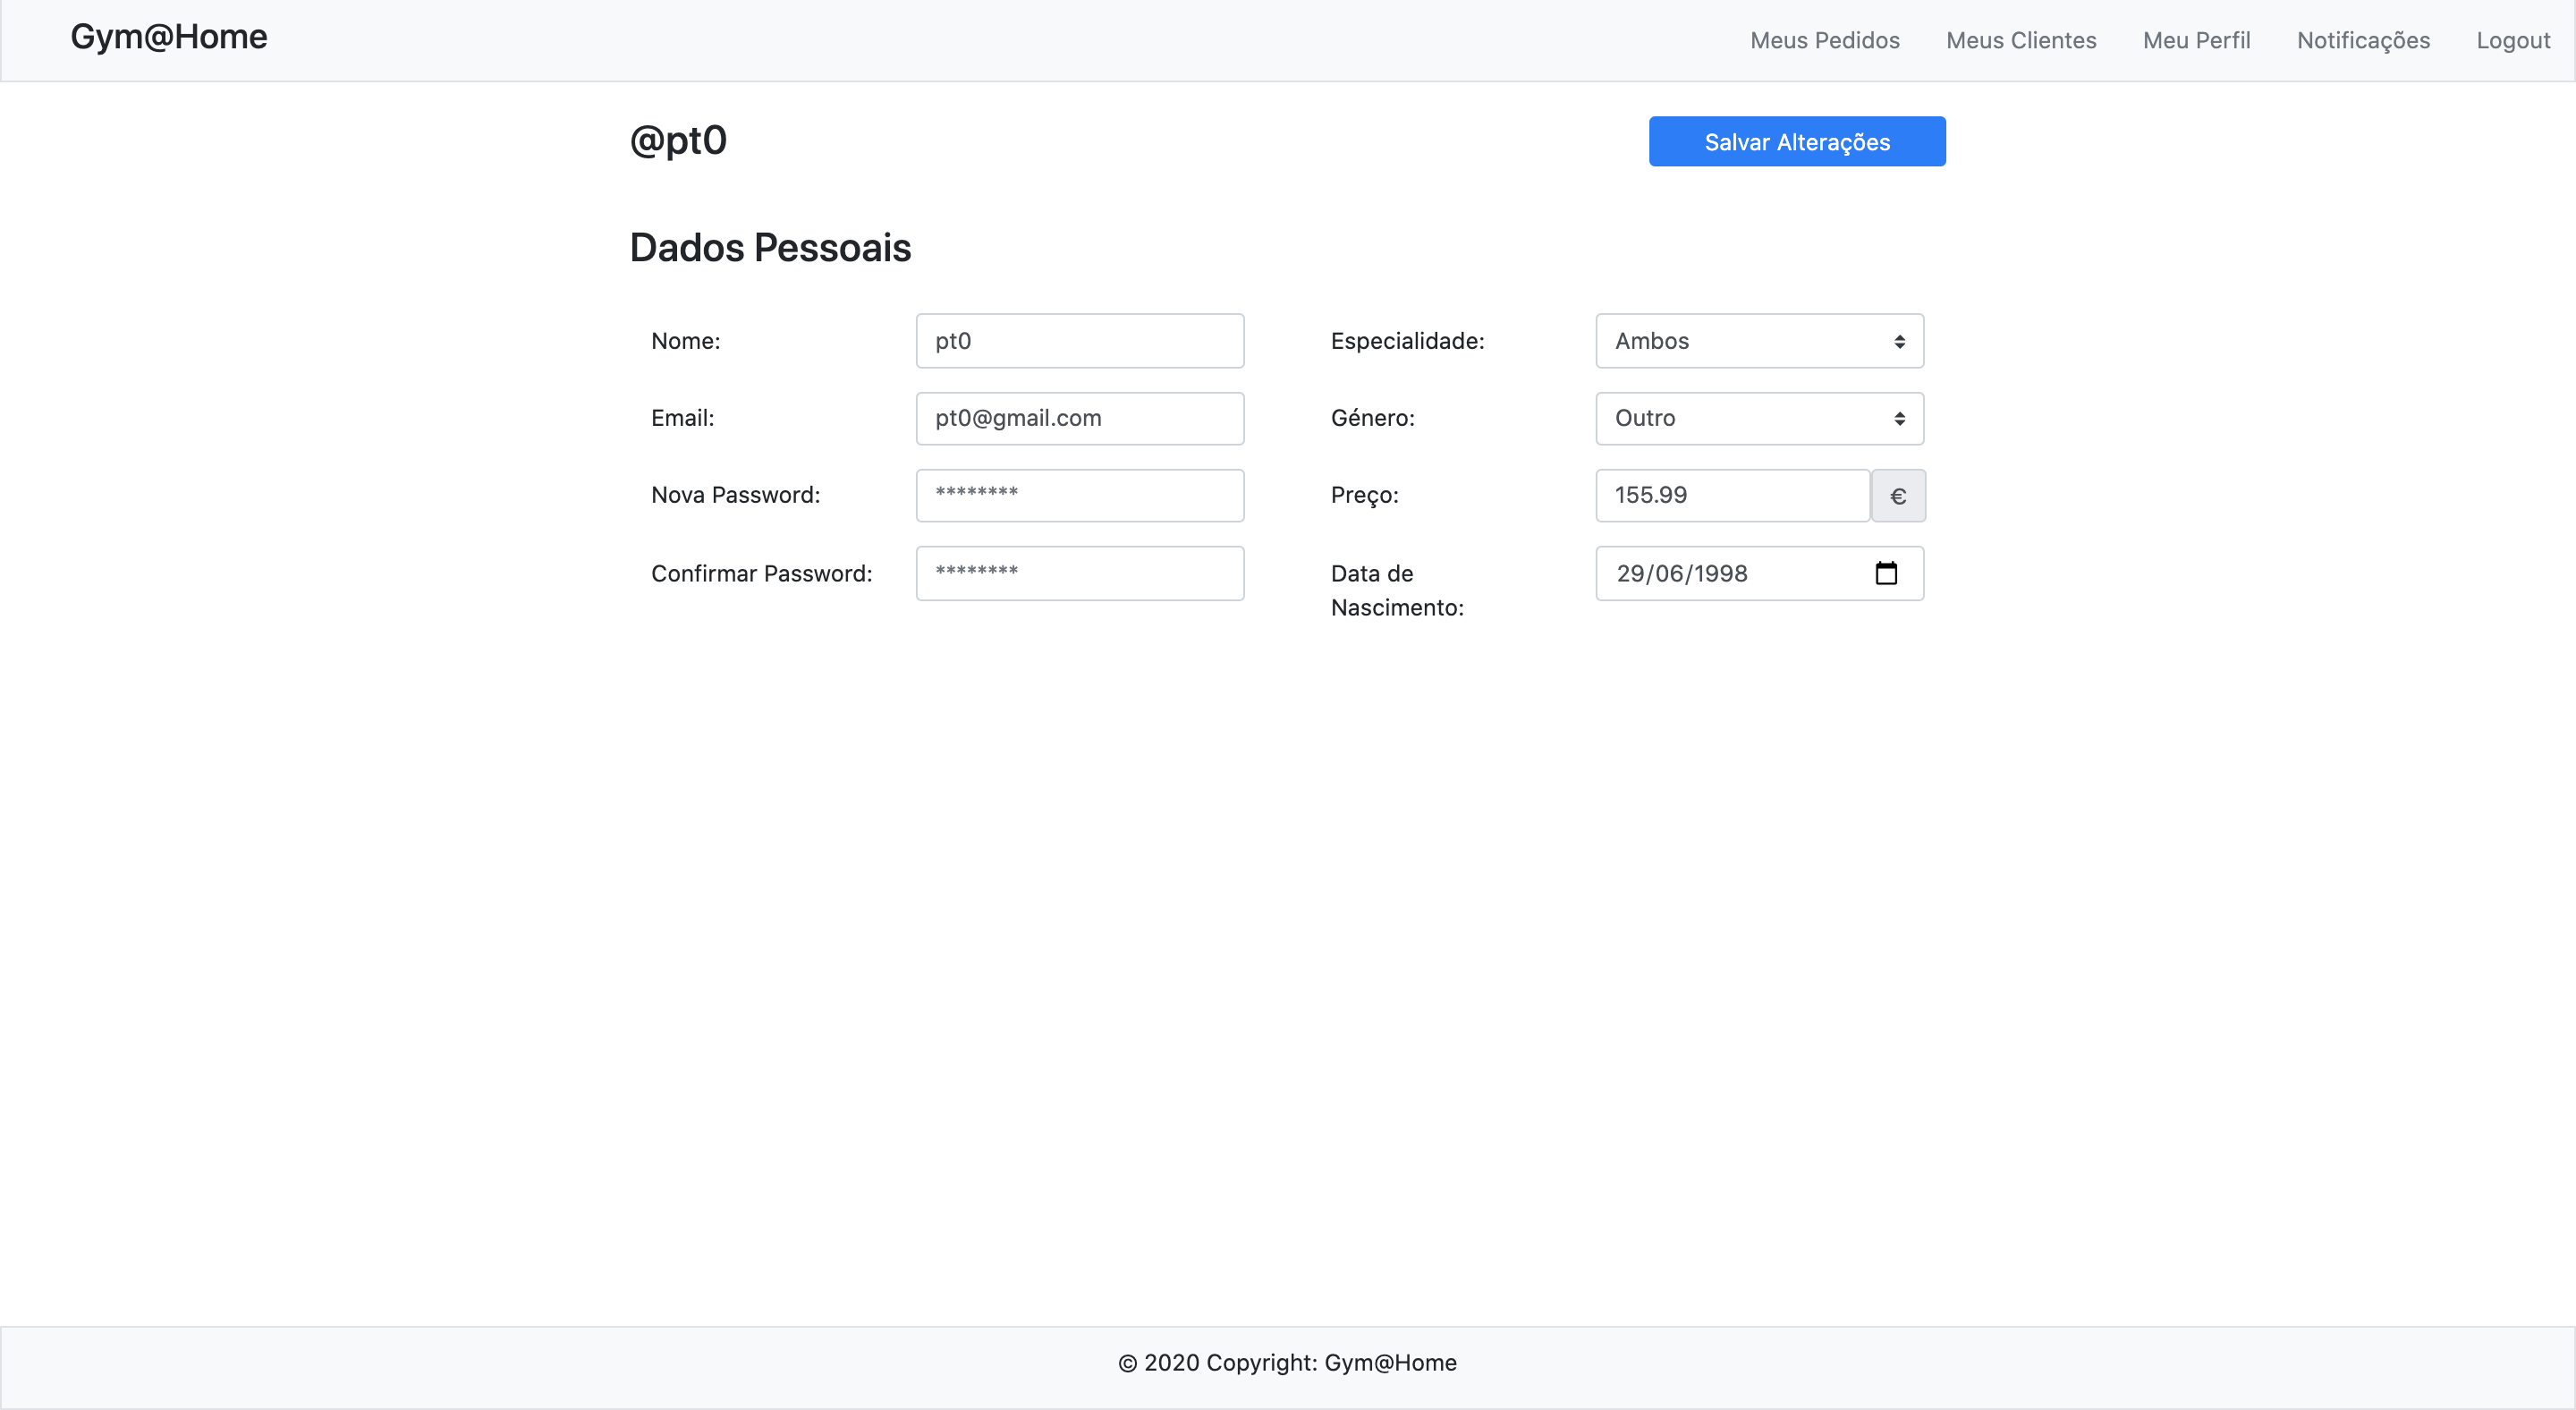
\includegraphics[scale=0.25]{images/interfaces/pt_perfil.png}
    \caption{Interface Perfil PT visto pelo próprio.}
    \label{fig:interfaceperfilptbypt}
\end{figure}

\subsubsection{Princípios de usabilidade}
\begin{itemize}
   \item \textbf{Substitutivity}: Os inputs da interface onde o PT pode alterar os valores são também outputs. Sempre que o PT alterar dados estes são guardados na BD e novamente carregados para os outputs que o PT tinha utilizado como input.
    
    \item \textbf{Observability}: O botão "Salvar Alterações" está no cimo da página para o PT o conseguir observar mal carregue a página.
    
    \item \textbf{Familiarity}: Colocar a "Data de Nascimento" é feito através de um calendário, pelo que o PT como ser humano está mais familiarizado a utilizar.
\end{itemize}

\subsubsection{Heurísticas de Normam}
\begin{itemize}
    \item \textbf{Error prevention}: Todos os inputs numéricos aceitam apenas números, o "Género" e "Especialidade" apenas permite os valores dos dropdowns, a "Data de Nascimento" apenas permite datas seleccionadas pelo calendário e o "Email" apenas aceita um email (tem de conter o @).
    \item \textbf{Flexibility and efficiency of use}: tal como diz respeito ao principio \textbf{Substitutivity}, usar o mesmo componente quer para visualizar, quer para editar o perfil, torna a interface mais eficiente para o PT.
\end{itemize}

\subsection{Consulta do perfil do Cliente pelo PT}
\label{subsec:perfilclientbypt}

\subsubsection{Descrição}
\hspace{5mm} Com o objectivo de facilitar o acesso rápido às informações do Cliente sem ter que ir para uma nova página e voltar, colocou-se um botão/atalho, que mostra os mesmos num pop-up, sendo isto possível e consistente em diversas interfaces, sendo que no lado do PT será no "Meus Clientes" e "Meus Pedidos de Clientes". 

\hspace{5mm} Assim reduziu-se a quantidade de cliques necessários para aceder aos dados, desta forma, acha-se que foi um boa melhoria, principalmente no ponto de vista do PT que fará esta acção repetitivamente, tornando assim a utilização da aplicação mais eficiente. 

\hspace{5mm} A alteração para pop-up, torna-se bastante diferente do protótipo, no entanto, as alterações na opinião da equipa foram para melhorar.

\begin{figure}[H]
    \centering
    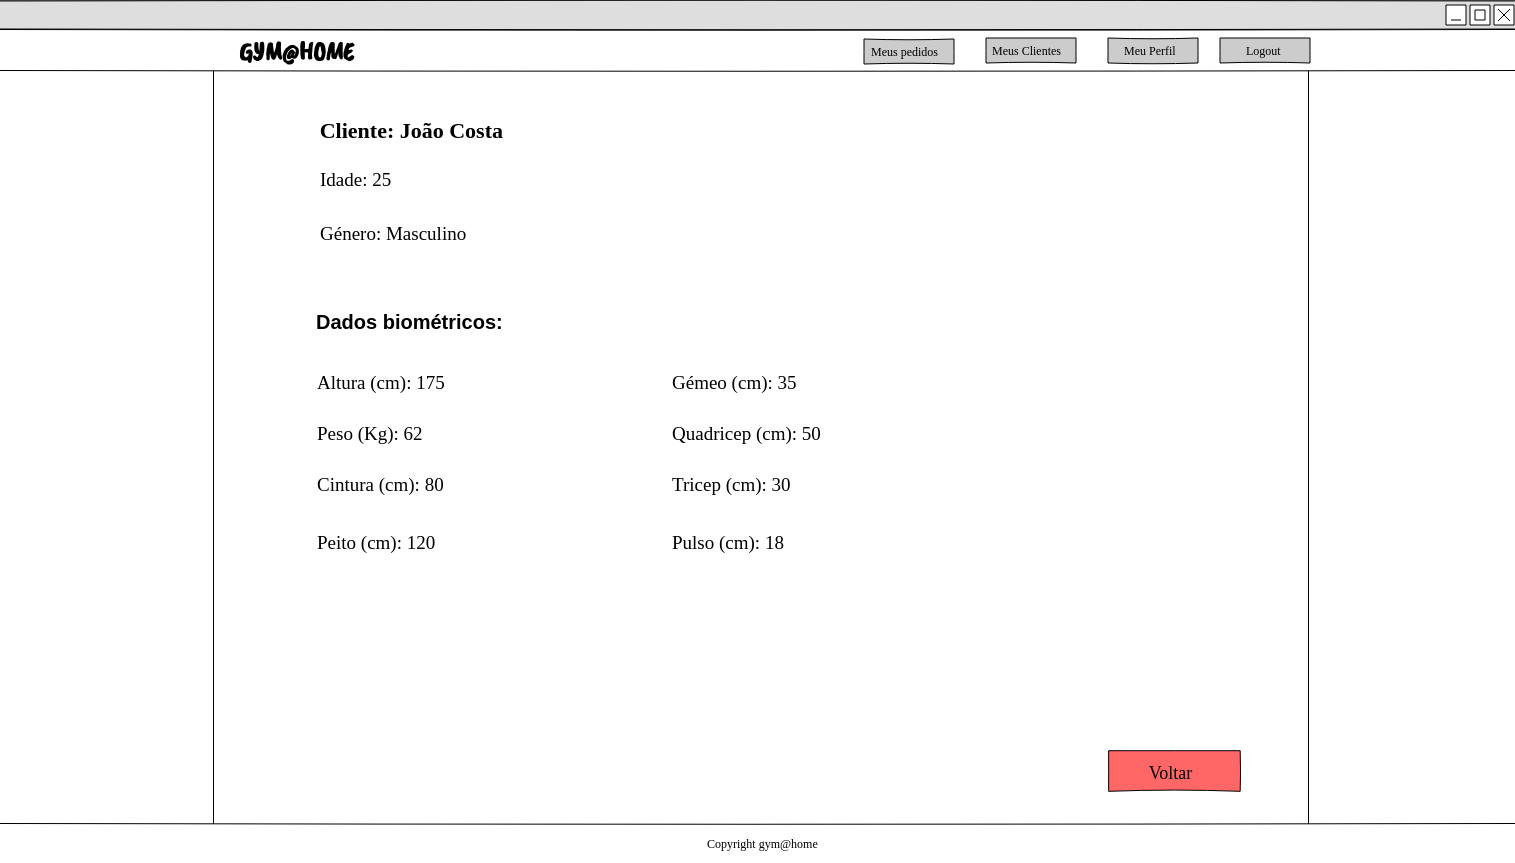
\includegraphics[scale=0.25]{images/mockups/pt_dados_cliente.png}
    \caption{Mockup Perfil Cliente visto pelo PT.}
    \label{fig:mockupperfilclientebypt}
\end{figure}

\begin{figure}[H]
    \centering
    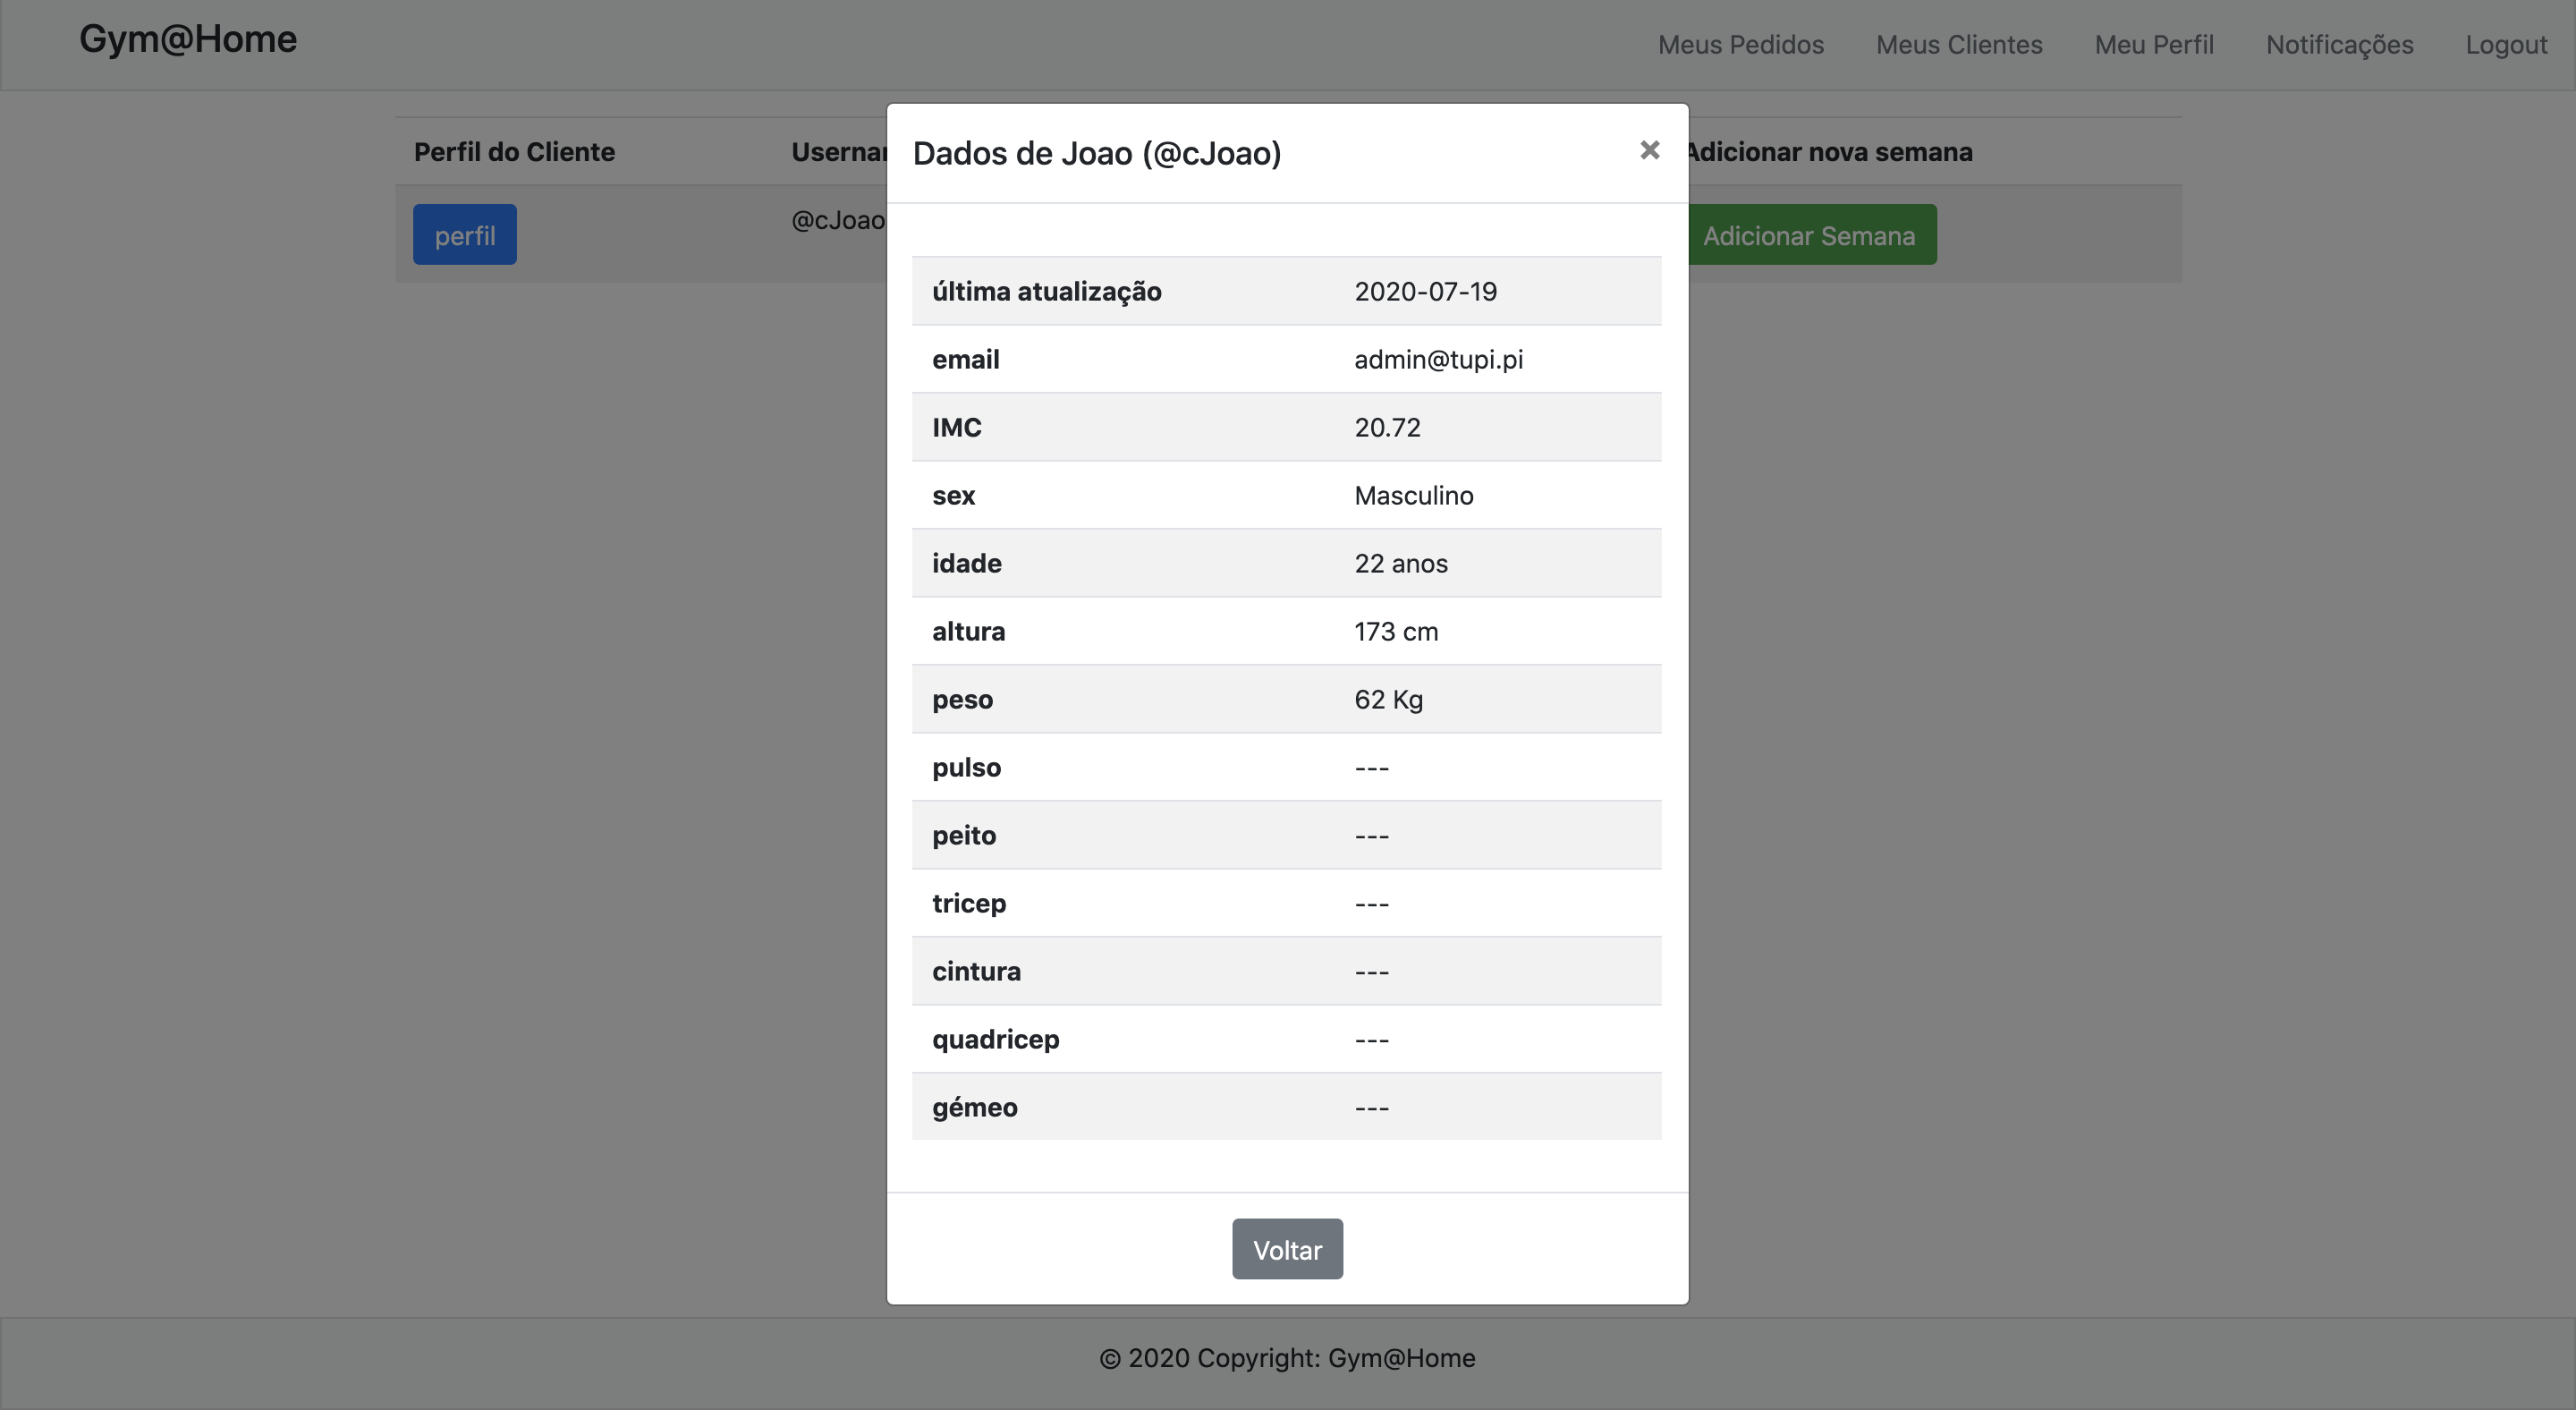
\includegraphics[scale=0.25]{images/interfaces/pt_perfil_cliente.png}
    \caption{Interface Perfil Cliente visto pelo PT.}
    \label{fig:interfaceperfilclientebypt}
\end{figure}

\subsubsection{Princípios de usabilidade}
\begin{itemize}
    \item \textbf{Consistency}: na medida em que, mantêm-se sempre a mesma forma de apresentar o perfil (pop-up) nas várias views que necessitem dessa informação. Pode-se também considerar consistente devido ao facto de a apresentação do perfil do PT ter a mesma estrutura mas com campos diferentes.
    
    \item \textbf{Flexibility and efficiency of use}: o botão "perfil", que mostra as informações do Cliente torna esse processo de consulta mais \textbf{eficiente}, como uma espécie de atalho.
\end{itemize}

\subsubsection{Heurísticas de Normam}
\begin{itemize}
    \item \textbf{Consistency and Standards}: devido à consistência da mesma forma de apresentação pelas várias mockups que necessitam de aceder à informação do cliente.
    \item \textbf{Flexibility and efficiency of use}: o botão de "perfil" presente em algumas interfaces que necessitam de consultar os dados do cliente, torna esse processo mais eficiente para o utilizador, neste caso para o PT. Principalmente para este utilizador, que poderá lidar com muitos pedidos de plano, e para tal precisará de consultar os dados dos clientes, e com apenas um clique consegue fazê-lo.
\end{itemize}

\subsection{Pedidos recebidos pelo PT}
\label{subsec:pedidosclientes}

\subsubsection{Descrição}
\hspace{5mm} Inicialmente importa referir que esta foi uma das interfaces que mudou drasticamente em relação ao prototipo, pois achou-se que não fazia sentido. Primeiramente a tabela lateral apenas tinha o nome do cliente, o que não é nada informativo para o PT. Depois, o PT tinha que clicar na tabela para ver os dados do formulário de cada cliente, o que não é \textbf{eficiente} para o mesmo. Do mesmo modo como já foi referido, o botão para consultar o perfil na página do cliente não é de todo a forma mais eficiente. 

\hspace{5mm}A solução para tornar esta interface mais eficiente, foi em listar os pedidos, bem como os dados mais importantes referentes ao pedido (campos do formulário), permitindo facilmente ao PT ver a informação de cada pedido sem necessitar de clicar em cada cliente. Isto permite por exemplo excluir alguns pedidos apenas olhando para estes dados da tabela. No entanto, consultar os dados biométricos 
é importante em certas situações para se decidir se aceita ou rejeita o pedido. Dessa forma, e como em outras views onde se necessita de consultar dados de perfil, colou-se um botão em cada pedido para aparecer um pop up com a informação do cliente. Como por vezes o PT pode decidir no momento em que consulta esses dados se vai aceitar ou rejeitar, logo, propaga-se os botões de aceitar ou rejeitar para esse pop-up.

\hspace{5mm} Após aceitar um pedido, será redireccionado para a interface "Criar uma semana do plano", caso rejeite, fica na mesma interface e o pedido é removido da tabela.

\begin{figure}[H]
    \centering
    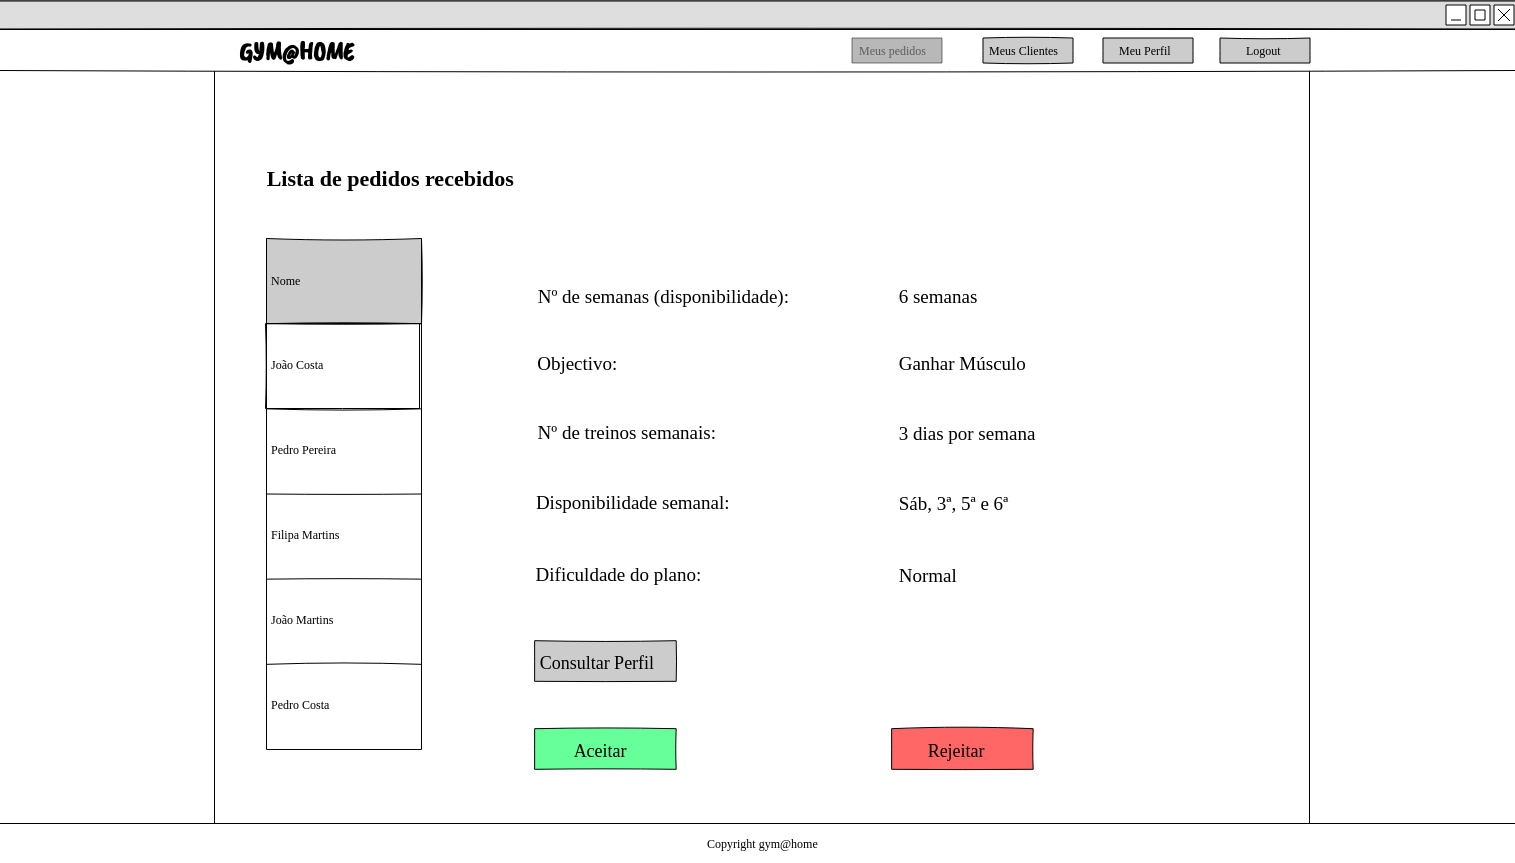
\includegraphics[scale=0.25]{images/mockups/pt_meus_pedidos_joo_costa.png}
    \caption{Mockup Pedidos Clientes.}
    \label{fig:mockuppedidosclientes}
\end{figure}

\begin{figure}[H]
    \centering
    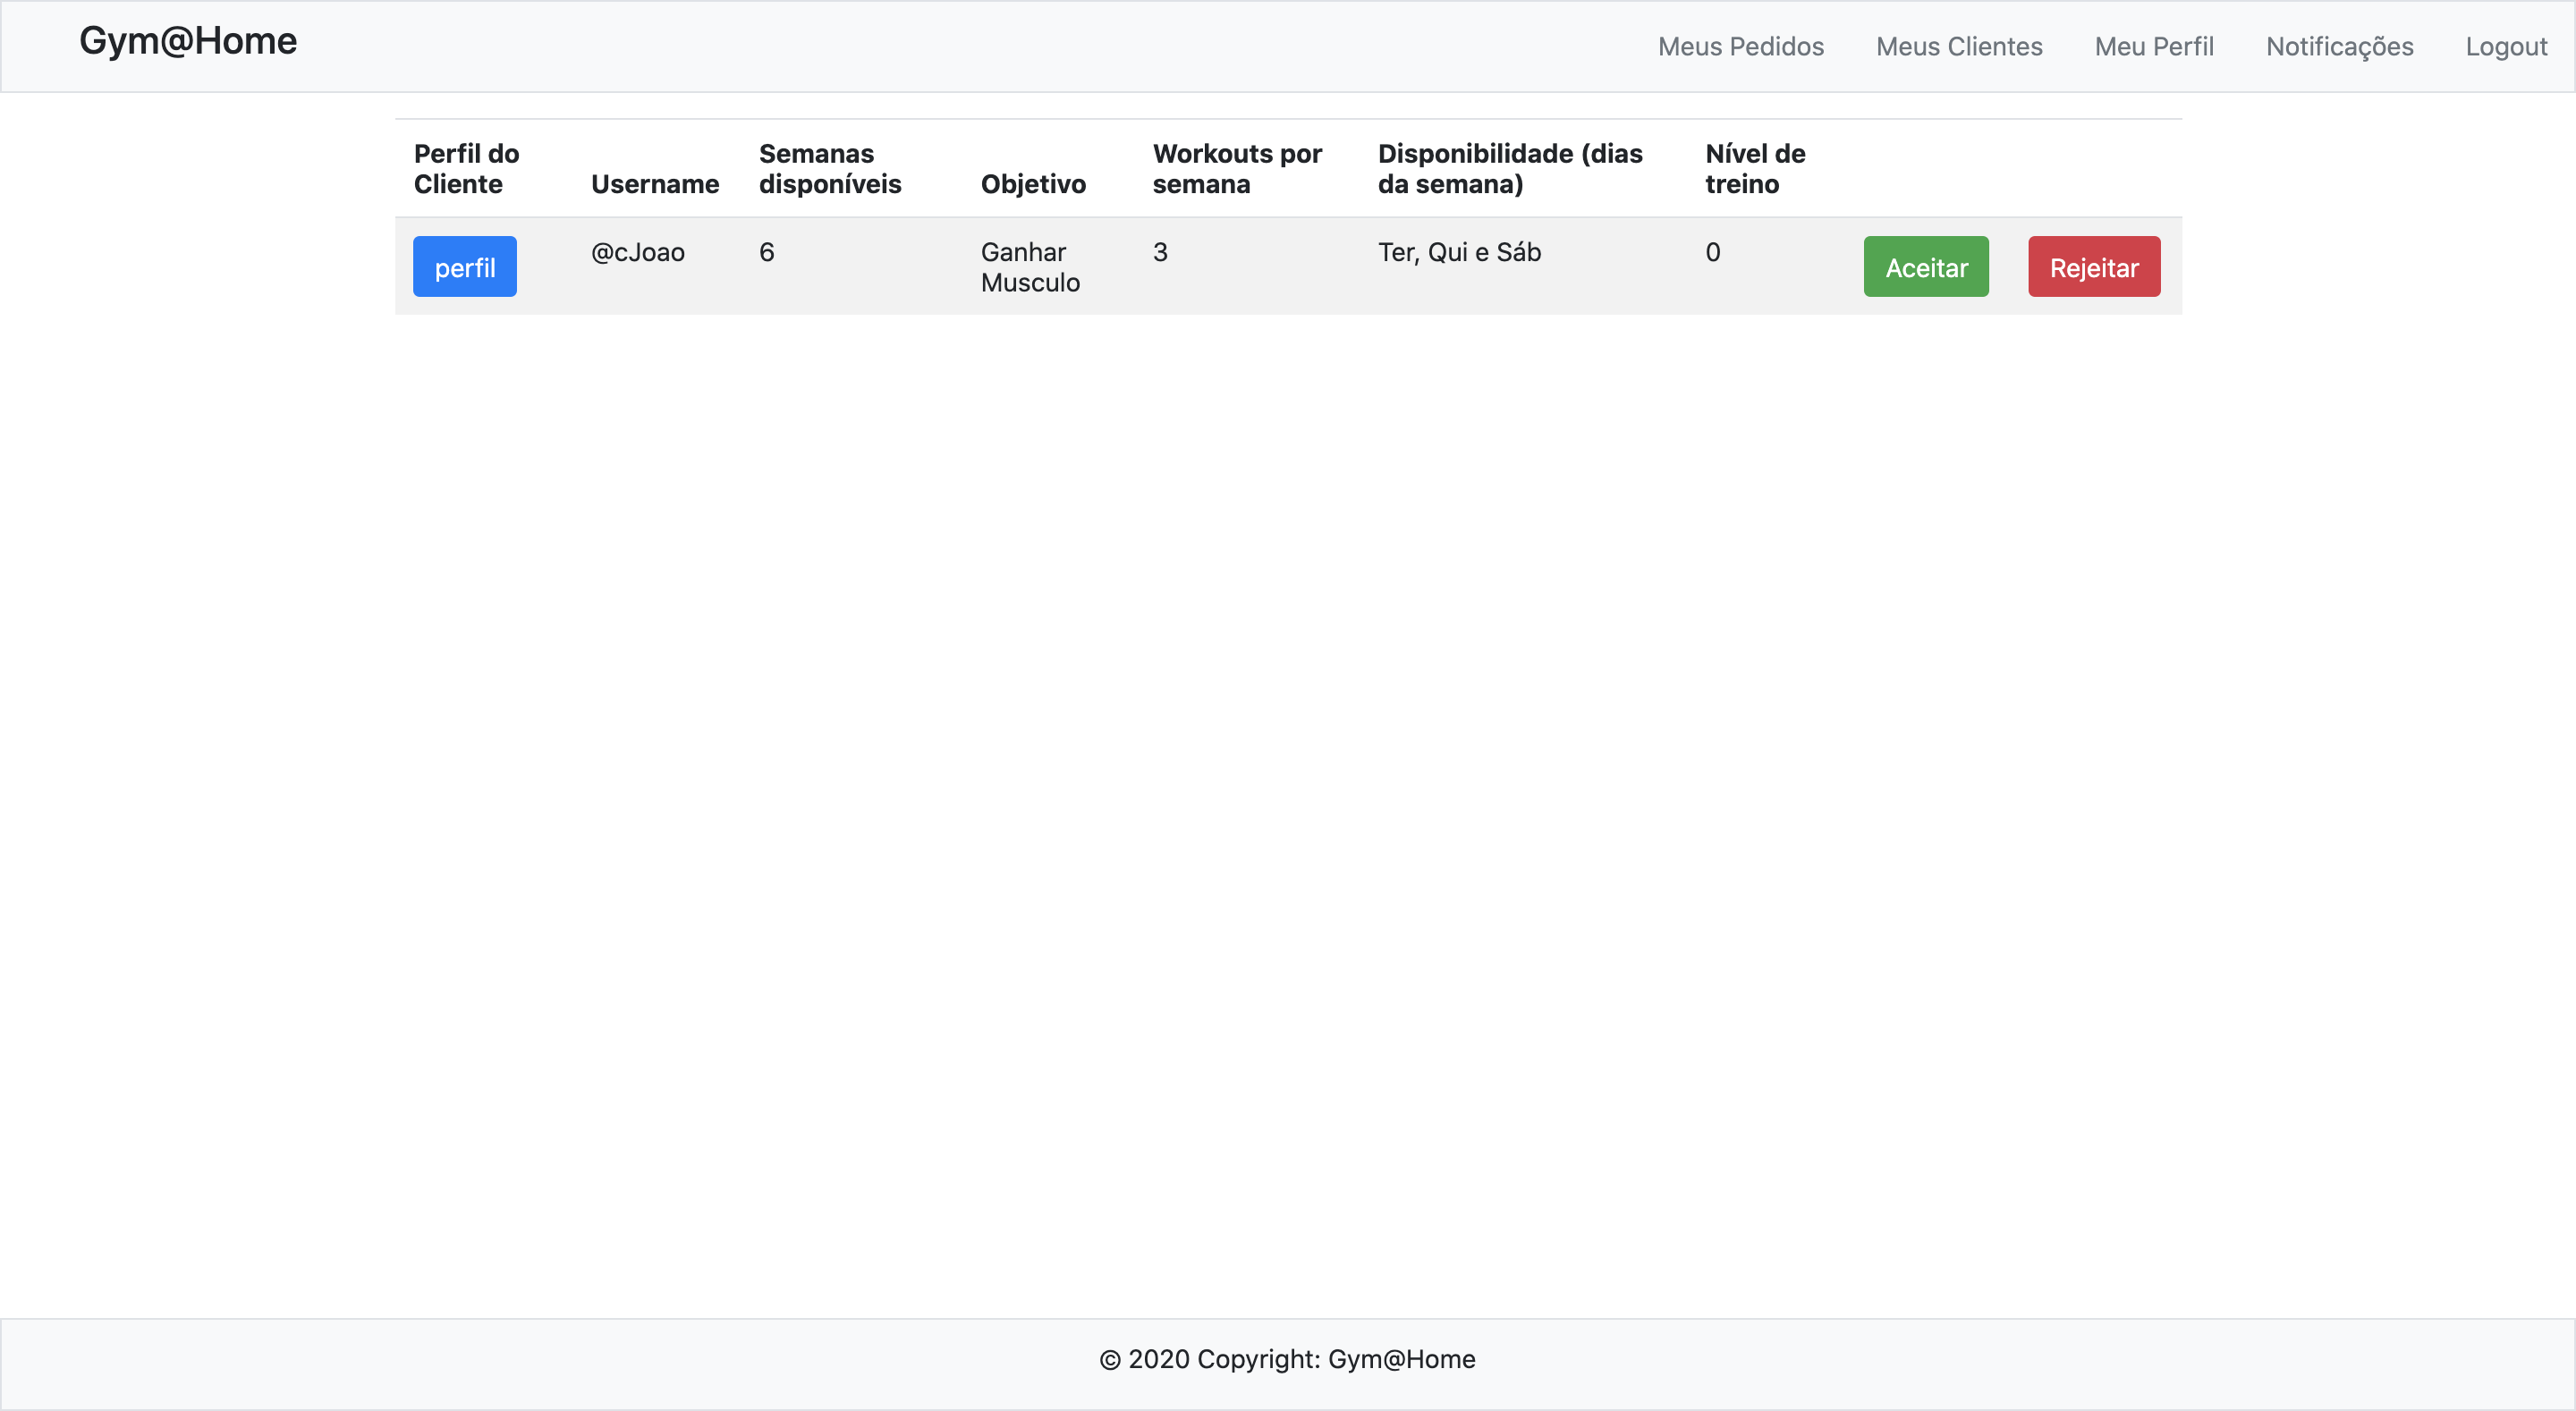
\includegraphics[scale=0.25]{images/interfaces/pt_meus_pedidos.png}
    \caption{Interface Pedidos Clientes.}
    \label{fig:interfacepedidosclientes}
\end{figure}

\subsubsection{Princípios de usabilidade}
\begin{itemize}
    \item \textbf{Synthesizability}: uma das acções possíveis nesta interface consiste em consultar o perfil do Cliente, pelo que após clicar no botão "perfil", aparece um pop-up com as informações do mesmo, ou seja, o PT consegue perceber o efeito das suas acções. Por outro lado, o botão aceitar, redireciona para a página "Criar semana do plano", logo, da mesma forma, o PT, também percebe o efeito da sua ação. Por fim, o rejeitar, marca o pedido como rejeitado, e o mesmo não aparecerá na tabela no próximo refresh, mostrando ao PT o efeito de ter rejeitado.
    \item \textbf{Generalizability} e \textbf{Consistency}: tal como já foi dito, o Cliente também contem uma interface para ver os pedidos enviados pelo o mesmo, que a nível de estrutura pode-se considerar bastante semelhante a este, difere apenas no conteúdos de algumas colunas, pelo que se pode considerar que se trata de uma interface genérica/consistente no sistema. 
    \item \textbf{Observability}: esta interface pode aumentar bastante o número de linhas da tabela, no entanto cada linha tem os botões para as acções desse pedido, o que significa que se houvesse uma tabela gigante, as acções possíveis estariam lá, não necessitando de subir a página ou outra forma para encontrar os botões. No entanto o grupo reconhece que aqui também seria um bom candidato a paginação, não sendo possível implementar face à falta de tempo, mas será uma boa actualização no futuro.
\end{itemize}

\subsubsection{Heurísticas de Normam}
\begin{itemize}
    \item \textbf{Recognition rather than recall}: o PT não precisa de memorizar as informações dos formulários no momento em que aceita, pois esses dados são enviados para a interface "Criar Semana do Plano".
    \item \textbf{Flexibility and efficiency of use}: o botão "perfil", que mostra as informações do Cliente torna esse processo de consulta mais \textbf{eficiente}, como uma espécie de atalho.
    
\end{itemize}

\subsection{Clientes do PT}
\label{subsec:clientes}
\subsubsection{Descrição}
\hspace{5mm} A interface permite ao PT ter acesso rápido a todos os seus Clientes, que tem actualmente, com a finalidade de ver o Plano de cada um, o perfil ou adicionar uma nova semana aos planos dos mesmos.

\hspace{5mm} Em cada linha da tabela, aparecem os botões referentes às funcionalidades referidas acima associados a cada cliente.

\begin{figure}[H]
    \centering
    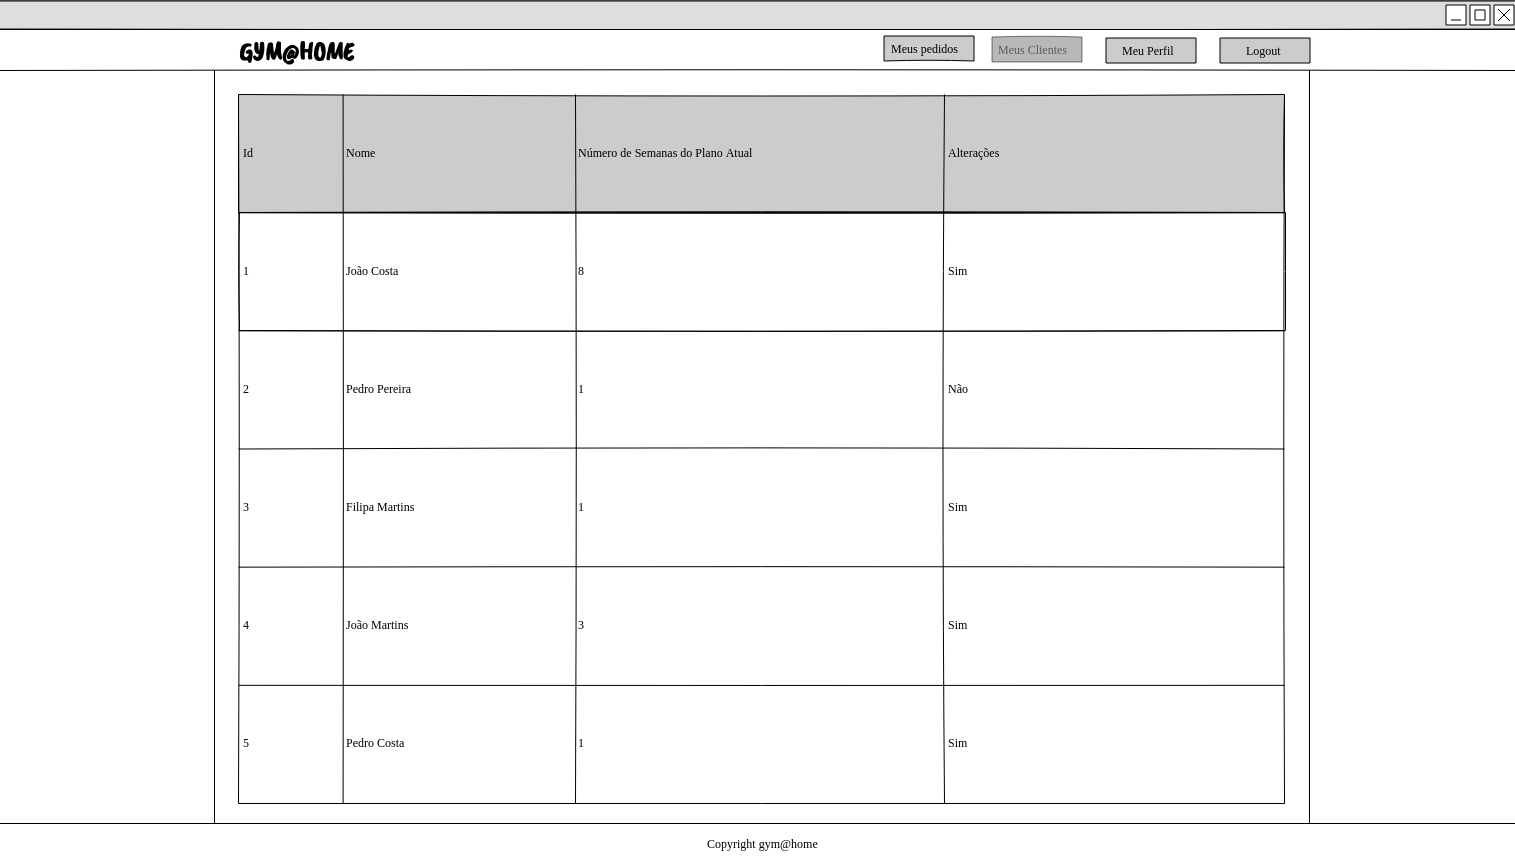
\includegraphics[scale=0.25]{images/mockups/personal_trainer_listar_clientes.png}
    \caption{Mockup Clientes do PT.}
    \label{fig:mockupclientes}
\end{figure}

\begin{figure}[H]
    \centering
    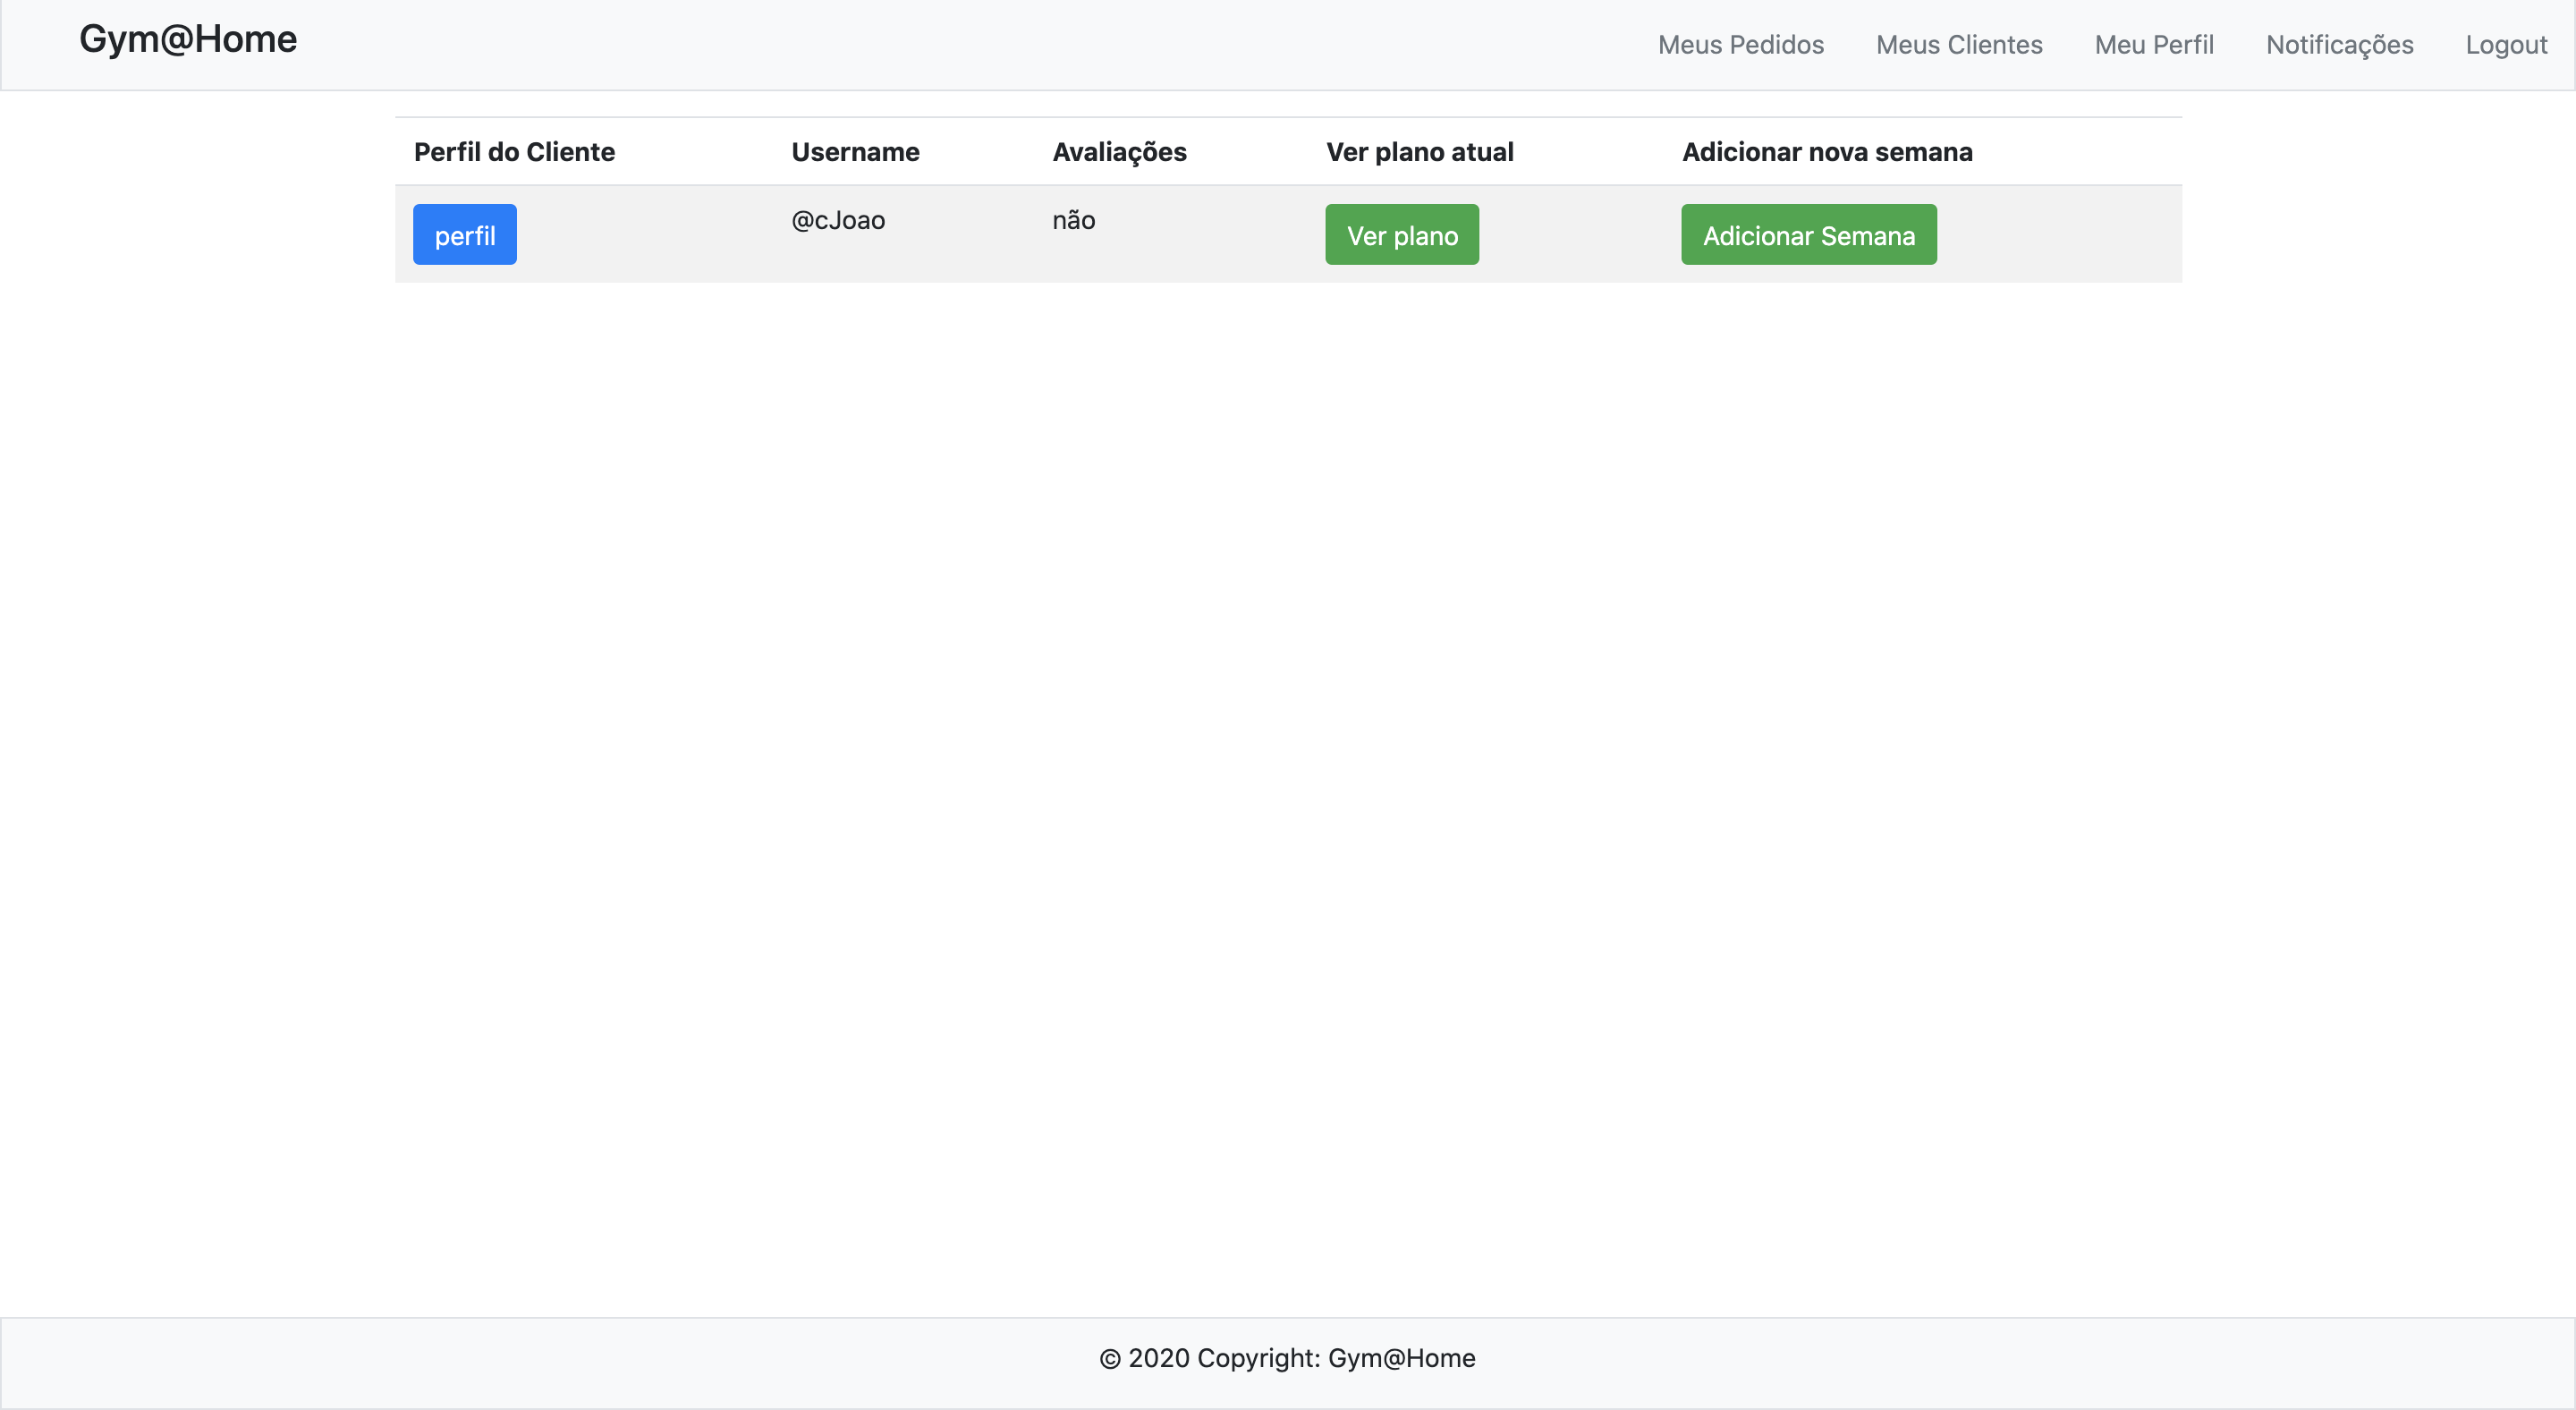
\includegraphics[scale=0.25]{images/interfaces/pt_meus_clientes.png}
    \caption{Interface Clientes do PT.}
    \label{fig:interfaceclientes}
\end{figure}

\subsubsection{Princípios de usabilidade}
\begin{itemize}
    \item \textbf{Synthesizability}: uma das acções possíveis nesta interface consiste em consultar o perfil do Cliente, pelo que após clicar no botão "perfil", aparece um pop-up com as informações do mesmo, ou seja, o PT consegue perceber o efeito das suas acções. Por outro lado, o botão ver plano, redirecciona para a página "Consultar Plano", logo, da mesma forma, o PT, também percebe o efeito da sua acção. Por fim, o adicionar semana, redirecciona para a página "Adicionar Semana", pelo que o PT percebe o efeito da sua acção.
    \item \textbf{Observability}: esta interface pode aumentar bastante o número de linhas da tabela, no entanto cada linha tem os botões para as acções desse cliente, o que significa que se houvesse uma tabela gigante, as acções possíveis estariam lá, não necessitando de subir a página ou outra forma para encontrar os botões. No entanto, o grupo reconhece que aqui também seria um bom candidato a paginação, não sendo possível implementar face à falta de tempo, mas será uma boa actualização no futuro.
\end{itemize}

\subsubsection{Heurísticas de Normam}
\begin{itemize}
    \item \textbf{Recognition rather than recall}: o PT não precisa de memorizar as informações do cliente no momento em que cria uma nova semana para o plano do mesmo , pois esses dados são enviados para a interface "Criar Semana do Plano".
    \item \textbf{Flexibility and efficiency of use}: o botão "perfil", que mostra as informações do Cliente torna esse processo de consulta mais \textbf{eficiente}, como uma espécie de atalho.
    
\end{itemize}

\subsection{Criar Semana}
\label{subsec:criarsemana}
\hspace{5mm} O workout "Criar Semana" foi um dos mockups que teve que ser revisto face à primeira fase de apresentação do projecto, após o conselho da equipa docente de repensar o mesmo, pois estava demasiado complexo, confuso e pouco usável. A equipa decidiu que teria de ser tudo feito numa única página. Dessa forma, Chegou-se ao resultado que se pode ver nas figuras \ref{fig:mockupcriarsemana} e \ref{fig:interfacecriarsemana}.

\hspace{5mm} Primeiramente, importa realçar o preload dos dados do formulário do cliente, importantes para saber criar a semana. À esquerda, tem-se uma tabela, com os workouts criados, sendo que inicialmente estará vazia. Depois tem-se a escolha do nome para o workout, bem como o dia da semana, sendo que este dropDown dos dias, vai automaticamente buscar os dias do formulário e reduzindo-os cada vez que se faz um workout. Por fim, tem-se uma tabela, super dinâmica, que aumenta e diminui de linhas, permitindo ao PT adicionar/remover o número de tarefas que pretender, não sendo um valor fixo.

\hspace{5mm} Importante realçar nesta interface que a semana só é guardada no momento em que clicar no botão guardar semana, caso contrário, tudo que foi criada é descartado. Como se trata de opções impossíveis de reverter, também são difíceis de realizar, pois aparece sempre um pop-up a perguntar se tem a certeza da acção.


\subsubsection{Descrição}
\hspace{5mm} 

\begin{figure}[H]
    \centering
    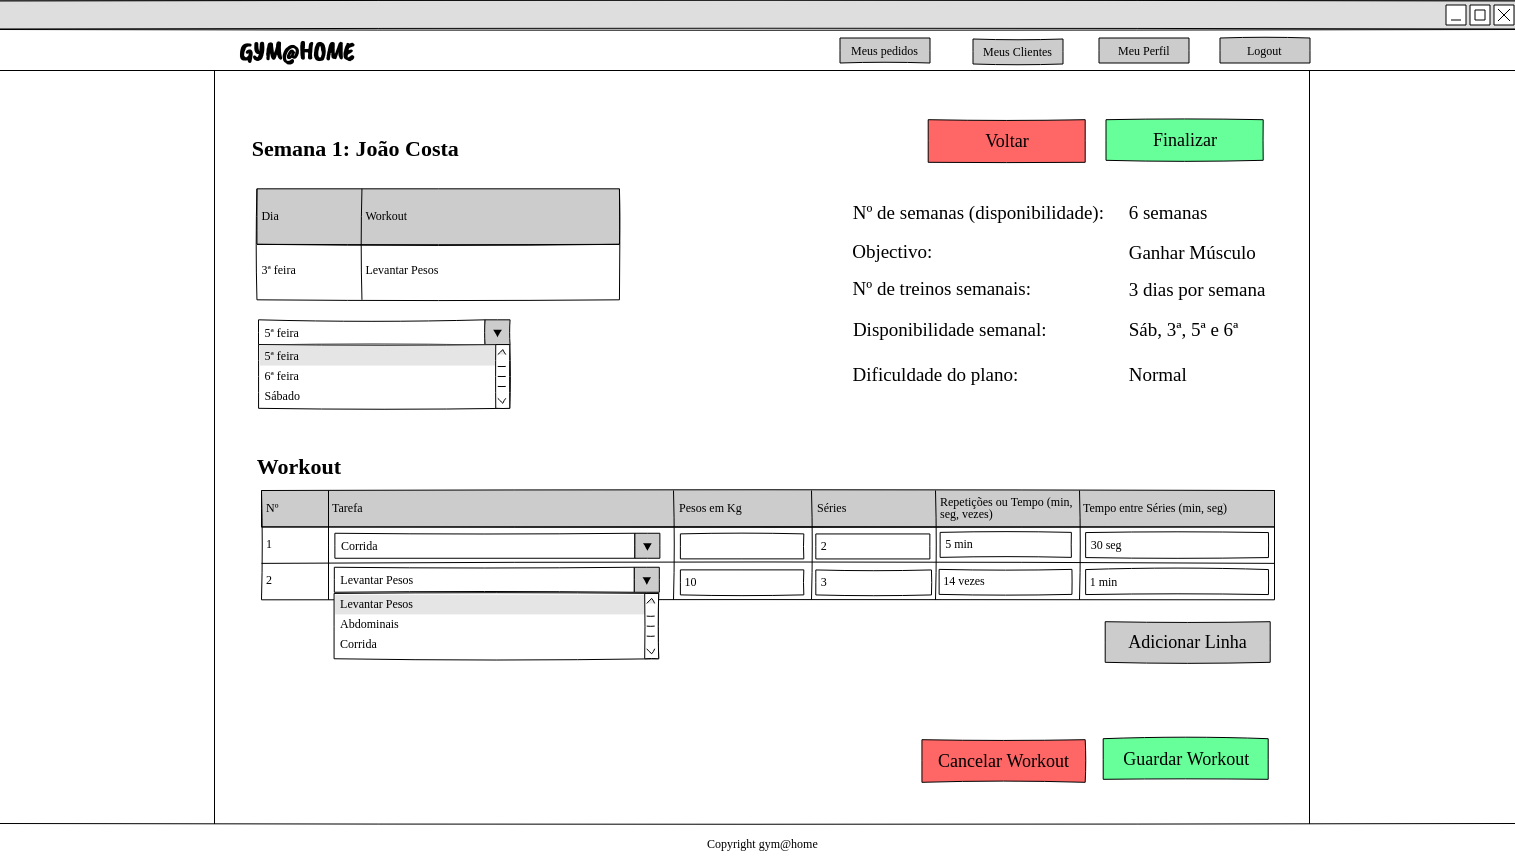
\includegraphics[scale=0.25]{images/mockups/pt_criar_semana.png}
    \caption{Mockup Criar Semana.}
    \label{fig:mockupcriarsemana}
\end{figure}

\begin{figure}[H]
    \centering
    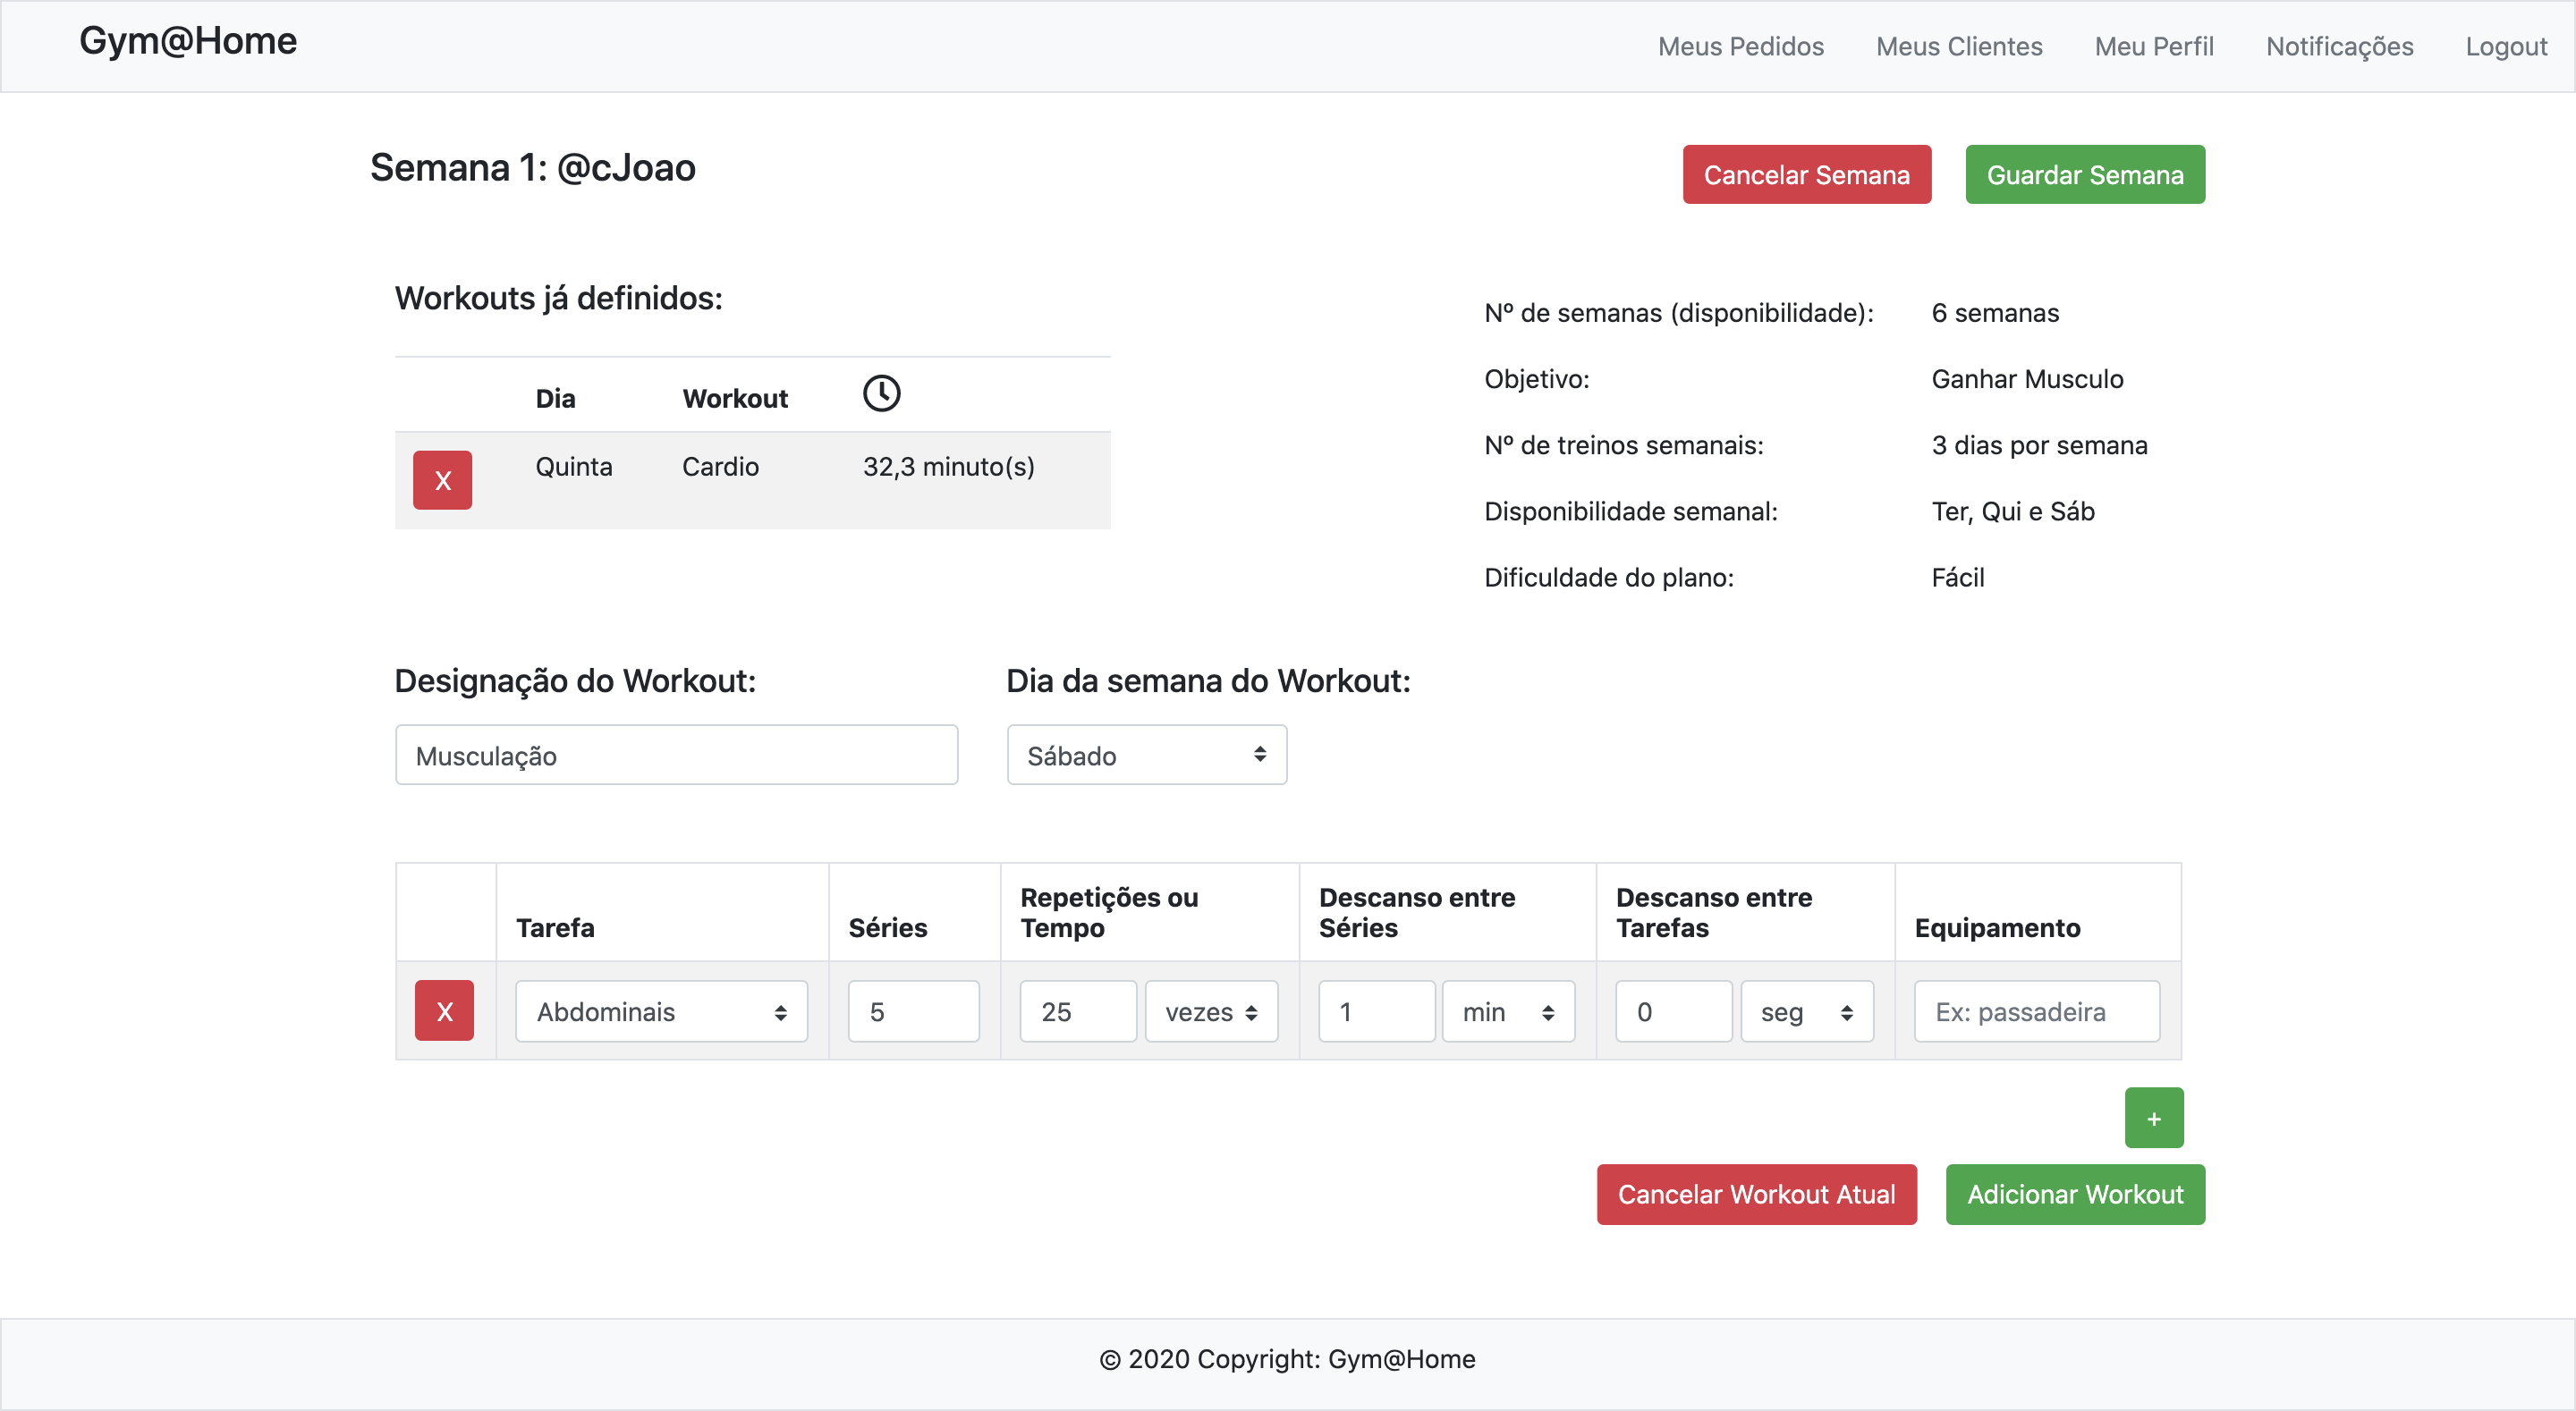
\includegraphics[scale=0.25]{images/interfaces/pt_criar_semana.png}
    \caption{Interface Criar Semana.}
    \label{fig:interfacecriarsemana}
\end{figure}

\subsubsection{Princípios de usabilidade}
\begin{itemize}
    \item \textbf{Substitutivity}: O PT pode definir um tempo em segundos ou em minutos.
    \item \textbf{Customizability}: pois o PT pode adicionar/remove mais linhas à tabela onde define as tarefas de um workout
    \item \textbf{Observability}: na medida em que, quando o PT guarda um workout, o mesmo faz \textbf{preload} na tabela que está no topo (tabela denominada, "wrokouts já definidos", podendo o mesmo observar os workouts que já definiu.
    \item \textbf{Recoverability}: a tabela onde estão os workouts já definidos permite apagar, ou seja, reverter. De modo semelhante, o botão "Cancelar workout" também reverte a tabela onde se define as tarefas.
\end{itemize}

\subsubsection{Heurísticas de Normam}
\begin{itemize}
    \item \textbf{Recognition rather than recall}: Os dados do pedido do Cliente são ilustrados durante a criação da semana para o PT não ter de se lembrar de quais eram os requisitos do pedido.
    
    \item \textbf{Error prevention}: Todos os inputs numéricos aceitam apenas números. Não é permitido ao PT "Guardar Semana" se a Semana não tiver nenhum Workout criado para a mesma.
\end{itemize}

\subsection{Semana do Cliente vista pelo PT}
\label{subsec:semanacliente}

\subsubsection{Descrição}
\hspace{5mm} A mockup é completamente análoga à "Semana" vista pelo Cliente, a única diferença é que no PT aparece o nome do Cliente ao qual aquela Semana pertence.

\begin{figure}[H]
    \centering
    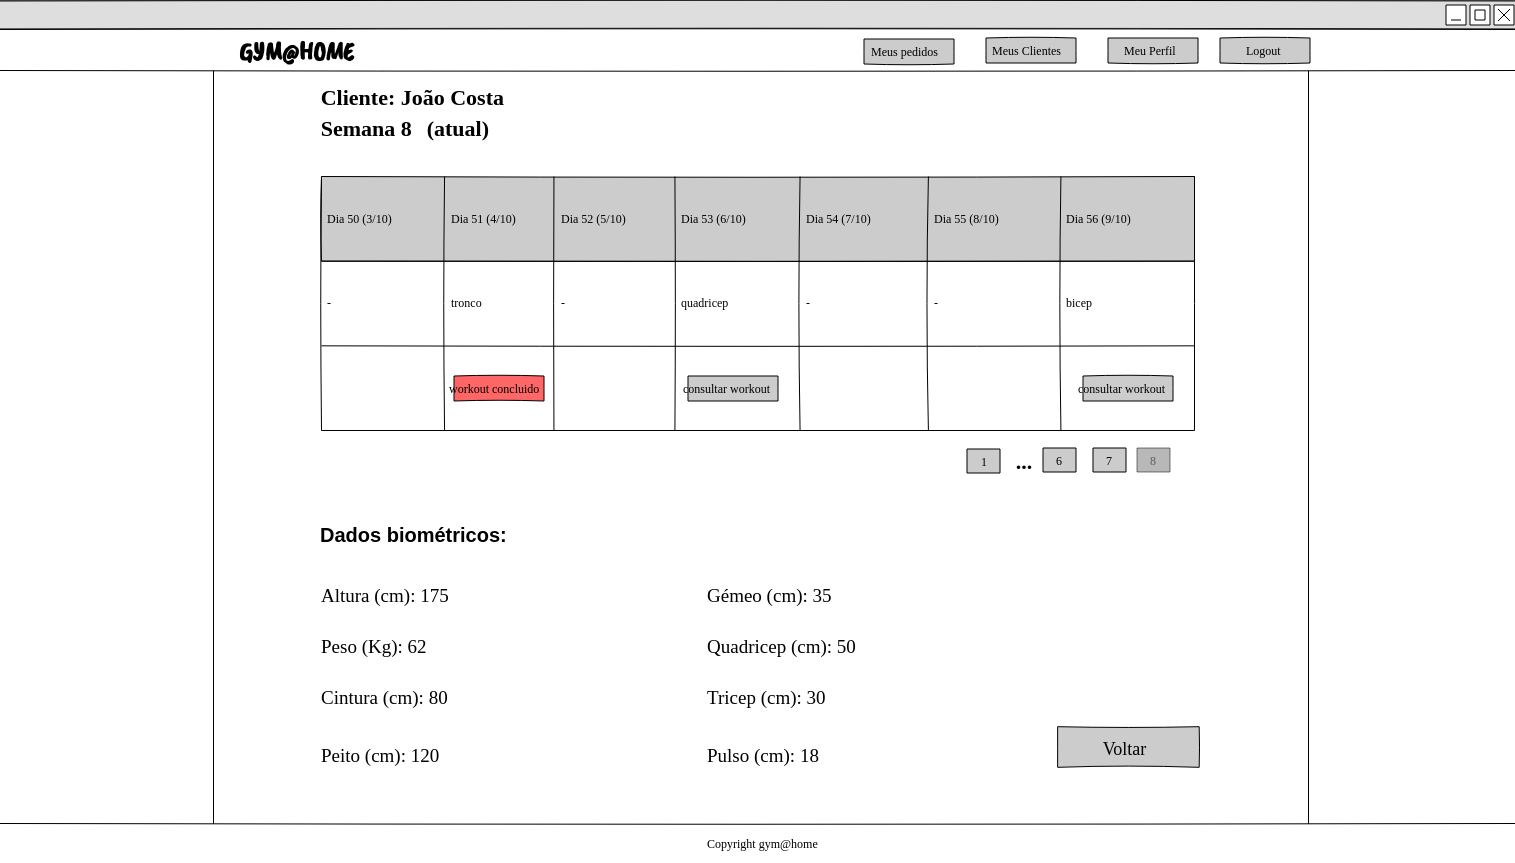
\includegraphics[scale=0.25]{images/mockups/pt_plano_do_cliente_semana_8_atual.png}
    \caption{Mockup Semana Cliente.}
    \label{fig:mockupsemanacliente}
\end{figure}

\begin{figure}[H]
    \centering
    \includegraphics[scale=0.25]{images/interfaces/pt_semana.png}
    \caption{Interface Semana Cliente.}
    \label{fig:interfacesemanacliente}
\end{figure}

\subsubsection{Princípios de Usabilidade}
\begin{itemize}
    \item \textbf{Observability}: Mais especificamente \textbf{Browsability} pois o PT consegue navegar entre as várias semanas do plano do Cliente.
    
    \item \textbf{Familiarity}: utilizou-se o formato semanal \textbf{comum/padrão} em horários e calendários, visto que é mais familiar aos utilizadores.
    
    \item \textbf{Generalizability} e \textbf{Consistency}: visto que utilizou-se a mesma estrutura tanto para a consulta pelo PT, bem como pelo Cliente, apesar de terem algumas diferenças, manteve-se a estrutura semanal, bem como os dados biométricos, excepto o botão de avaliação do PT, que não faz sentido no lado do PT.
\end{itemize}

\subsubsection{Heurísticas de Normam}
\begin{itemize}
    \item \textbf{Recognition rather than recall}: Os dados biométricos do Cliente são ilustrados durante a visualização da semana para o PT não ter de se lembrar de quais eram os valores dos dados biométricos.
\end{itemize}

\subsection{Workout do Cliente visto pelo PT}
\label{subsec:workoutcliente}

\subsubsection{Descrição}
\hspace{5mm} Tal como na mockup anterior esta é totalmente análoga à do Cliente, sendo que nesta aparece o nome do Cliente e o \textbf{PT não pode finalizar Workout}.

\begin{figure}[H]
    \centering
    \includegraphics[scale=0.25]{images/mockups/pt_plano_do_cliente_tarefa_1.png}
    \caption{Mockup Workout Cliente.}
    \label{fig:mockupworkoutcliente}
\end{figure}

\begin{figure}[H]
    \centering
    \includegraphics[scale=0.25]{images/interfaces/pt_workout.png}
    \caption{Interface Workout Cliente.}
    \label{fig:interfaceworkoutacliente}
\end{figure}

\subsubsection{Princípios de usabilidade}
\begin{itemize}
    \item \textbf{Observability}: Mais especificamente \textbf{Browsability} pois o PT consegue navegar entre as várias tarefas de um workout.
    
    \item \textbf{Generalizability} e \textbf{Consistency}: visto que utilizou-se a mesma estrutura tanto para a consulta pelo Cliente, bem como pelo PT, apesar de terem algumas diferenças, manteve-se a estrutura tabelar das séries de uma tarefa, bem como as informações da tarefa, considerando-se assim que torna-se genérica para ambos os utilizadores.
\end{itemize}

\subsubsection{Heurísticas de Normam}
\begin{itemize}
    \item \textbf{Recognition rather than recall}: as informações sobre o dia da semana e a definição do workout são passadas para esta view para que o cliente/PT não necessitem de memorizar.
\end{itemize}

%--------------------------------------------------------------------------%

\section{Alertas}
\label{sec:alertas}

\hspace{5mm} Algumas acções são impossíveis de reverter, dessa forma, deve-se dificultar as mesmas. Assim, foi criado o alerta de \textbf{confirmação} para ter a certeza que o utilizador pretende executar a acção.

\begin{figure}[H]
    \centering
    \includegraphics[scale=0.45]{images/alerts/alerta_confirmacao.png}
    \caption{Alerta de Confirmação.}
    \label{fig:alertaconfirmação}
\end{figure}
\chapter{Deployment}
\label{chap:instalacao}

\section{Ficheiros de configuração necessários para o deployment}

\hspace{5mm} A colocação da arquitectura em funcionamento necessita de um deployment de todos os componentes, sendo de preferência um processo automatizado. 

\hspace{5mm} Inicialmente foi necessário criar as imagens de todos os componentes desenvolvidos pela equipa. Na verdade, consiste em criar uma ficheiro Dockerfile tal como se pode observar na figura \ref{fig:dockerfile}. Nestas imagens necessita-se do servidor web, neste caso \textbf{wildlfy}, versão 12, que é automaticamente descarregado da internet. De seguida, necessita-se do ficheiro \textbf{.war} do projecto \textbf{NetBeans} do serviço, que será copiada para a pasta deployments do servidor web. Após a criação do ficheiro Dockerfile, necessita-se garantir que os ficheiros necessários para a criação da imagem estão juntamente com o ficheiro.

\begin{figure}[H]
    \centering
    \includegraphics[scale=0.40]{images/deployment/dockerfile.png}
    \caption{Exemplo de um dockerfile para um serviço do backend.}
    \label{fig:dockerfile}
\end{figure}

\hspace{5mm} De seguida, após concluir a criação de todos os dockerfiles, procede-se à criação do ficheiro de configuração denominado docker-compose.yml, que contém os serviços da arquitetura. Alguns serviços serão externos, tais como as BDs associadas a cada um dos sete serviço desenvolvido pelo grupo. A imagem dessas BDs será descarregada de um repositório, sendo que a mesma foi criada pela equipa de desenvolvimento do \textbf{MySQL}.

\hspace{5mm} A ferramenta docker tem a grande vantagem na criação de containers, que de uma forma sucinta, isolam um serviço com as dependências necessárias para o mesmo, permitindo facilidade na instalação de serviços.

\hspace{5mm} Uma grande vantagem da utilização do docker, consiste na criação de uma rede interna, onde todos os containers comunicam através da mesma, contendo até um servidor DNS, o que significa que para fazer a comunicação entre dois serviços basta utilizar o nome que lhes foi dado ao serviço, tal como se pode verificar na figura \ref{fig:dns-docker}, onde se faz a conexão a uma base de dados usando o nome do serviço \textbf{clientdb}. Assim, esta característica facilita na criação do docker-compose.yml.

\begin{figure}[H]
    \centering
    \includegraphics[scale=0.30]{images/deployment/dns-docker.png}
    \caption{Utilização do nome do serviço docker para conectar a base de dados.}
    \label{fig:dns-docker}
\end{figure}

\hspace{5mm} O ficheiro de configuração docker-compose.yml define os serviços a fazer deployment, onde se especifica o nome, a localização da imagem/dockerfile, portas, entre outras variáveis importantes. Na \ref{fig:docker-compose}, o quadrado azul representa um serviço para adminitração das base de dados. O quadrado vermelho corresponde ao serviço frontend. O quadrado amarelo, corresponde ao serviço GymAtHome, que consiste no servidor \textbf{API} do backend, ou seja, o serviço responsável por fazer o dispatcher dos pedidos. Por fim, a verde tem-se um exemplo de um serviço do backend, responsável por guardar e gerir os planos. Todos os restantes serviços desenvolvidos pela equipa, são idênticos a este último, mudando apenas o nome do serviço, da imagem e  base de dados.

\hspace{5mm} Com a finalidade de facilitar/automatizar o processo de deployment, o grupo desenvolveu um makefile, que faz todos os comandos necessários para obter os .wars mais recentes, bem como executar o comando \textbf{docker-compose up -d --build}, para efetuar o deployment.

\begin{figure}[H]
    \centering
    \includegraphics[scale=0.45]{images/deployment/docker-compose.png}
    \caption{Ficheiro docker-compose.yml (o ficheiro tem os restantes serviços, no entanto, para explicar basta apenas esta parte do ficheiro).}
    \label{fig:docker-compose}
\end{figure}


\section{Processo deployment}

\hspace{5mm} Nesta secção apresenta-se o processo necessário para fazer deployment da aplicação.

\subsection{Requisitos}

\begin{itemize}
    \item docker
    \item diretoria docker/
    \item postman (ou outra alternativa que permita fazer HTTP POST)
    \item makefile
\end{itemize}

\subsection{Passo a passo}
\begin{itemize}
    \item cd docker/
    \item make up
    \item no postman terá que ser feito um pedido post para \textbf{IP\_HOST:8081/GymAtHome/api/createdbs}, com o body em /aplication/json com o token = admin (em json), tal como se pode verificar na figura \ref{fig:postman}, para inicializar as base de dados.
    
    \begin{figure}[H]
        \centering
        \includegraphics[scale=0.45]{images/deployment/postman.png}
        \caption{Pedido feito no postman para inicializar as base de dados.}
        \label{fig:postman}
    \end{figure}
\end{itemize}

\hspace{5mm} Desta forma, verifica-se que o processo de deployment torna-se bastante automatizado, necessitando apenas de um comando e um pedido http no postname, sendo que este pedido só seria necessária na primeira vez para a criação dos schemas nas base de dados.

\section{Preparado para Docker Swarm}

\hspace{5mm} Apesar de não ter sido feito, os ficheiros de configuração (docker-compose.yml) estão preparados para colocar a aplicação em produção, por exemplo num \textbf{Docker Swarm} com várias máquinas virtuais em \textbf{Swarm}, onde todas as máquinas poderão alocar serviços da arquitectura, no entanto não foi possível conceber o \textbf{Docker Swarm} nesta fase do projeto. 

\hspace{5mm} Outra nota importante consiste em colocar as imagens no \textbf{DockerHub}, um repositório de imagens, para que seja ainda mais fácil o deployment, necessitando apenas do ficheiro de configuração e não das imagens.

\hspace{5mm} No entanto, como foi dito, neste momento o deployment não está a ser feito para um \textbf{Docker Swarm}, no entanto, está preparado para tal.
%\chapter{Testes de carga}
\label{chap:testes}

\hspace{5mm} Em qualquer sistema, após a criação e configuração do deployment automatizado é necessário efectuar \textbf{testes de carga} antes da produção, desta forma o grupo criou \textbf{6 casos de testes}.

\hspace{5mm} Foram testados os métodos login e create apenas no serviço do Personal Trainer \textbf{inferindo-se que o desempenho dos mesmos seriam idênticos} no serviço Client pois realizam lógica idêntica.

\hspace{5mm} \textbf{Note-se que o grupo tem consciência que caso este projecto fosse em ambiente profissional e realmente fosse para entrar em produção todos os micro-serviços seriam testados individualmente, inclusive com várias configurações dos recursos das máquinas utilizadas e da infraestrutura. No entanto, visto que o ambiente é académico e os testes de carga não são o principal objectivo de avaliação, decidiu-se simplificar os mesmos.}

\hspace{5mm} Para a execução dos testes utilizou-se a ferramenta \href{https://jmeter.apache.org}{apache jmeter} sendo esta escolhida porque o grupo já estava familiarizado com a mesma uma vez que a utilizou noutros projectos.

\hspace{5mm} Para a \textbf{automatização dos testes}, primeiramente foram definidos os 6 testes de carga e guardadas as suas configurações nos ficheiros \textbf{.jmx}. De seguida foram adicionadas opções num Makefile que executam os testes \textbf{individualmente ou todos sequencialmente} tal como a seguinte figura sugere.

\begin{figure}[H]
    \centering
    \includegraphics[scale=0.4]{images/jmeter.png}
    \caption{Makefile para automatização dos testes de carga.}
    \label{fig:makefile}
\end{figure}

\hspace{5mm} Tal como se pode observar na figura o micro-serviços foram testados para \textbf{100, 250 e 500 personal trainers}. Todos os resultados obtidos serão colocados em anexo, no entanto nesta secção apenas serão abordados os resultados para 500 clientes.

\hspace{5mm} Os métodos testados  foram o \textbf{HTTP POST /PersonalTrainer/api/login} e o \textbf{HTTP POST /PersonalTrainer/api/createPersonalTrainer}. O conteúdo json enviado para cada um foi previamente calculado (no povoamento automático da base de dados) e de modo a simular a utilização real do sistema cada thread do jmeter (que representa um personal trainer a aceder ao sistema) contém um json específico que se encontra num ficheiro pts-data.csv.


\subsection{login para 500 Personal Trainers}

\hspace{5mm} Os dados obtidos para o teste do login para 500 Personal Trainers foram os seguintes.

\begin{figure}[H]
    \centering
    \includegraphics[scale=0.45]{images/login-500-pts.png}
    \caption{login para 500 Personal Trainers}
    \label{fig:login500}
\end{figure}

\hspace{5mm} \textbf{Note-se que o valor máximo para o tempo de resposta foi um pedido que demorou 5601 ms a ser processado, no entanto pode ser considerado um \href{https://en.wikipedia.org/wiki/Outlier}{outlier} uma vez que o percentil 99th indica que 99\% dos pedidos foram processados em menos de 765.75 ms, sendo um tempo de resposta útil.}
\input{body/conclusão.tex} 

\end{document}
